\documentclass{article}
\usepackage{mystyle}
\usepackage{amsmath, amssymb, amsfonts, amsthm, mathtools}
\usepackage[utf8]{inputenc}
\usepackage[inline]{enumitem}
\usepackage{cancel}
\usepackage{soul}
\usepackage{hyperref}
\usepackage{tikz-cd}
\usepackage{tikz}
\usetikzlibrary{decorations.markings, decorations}
\usetikzlibrary{arrows, positioning}
\usepackage{changepage}
\usepackage{subcaption}
\usepackage[section]{placeins}
\usepackage{lipsum, caption, graphicx, nicefrac}
\usepackage{float}
\usepackage{commath}
\usepackage[nottoc,notlot,notlof]{tocbibind}
%\usepackage[siunitx]{circuitikz}
\restylefloat{figure}
\usepackage{adjustbox}
\usepackage{color}
\usepackage[useregional, showdow]{datetime2}
\usepackage{colortbl}
\colorlet{shade}{gray!40}
\usepackage{xcolor}

\theoremstyle{definition}
\newtheorem{theorem}{Theorem}[subsection]
\newtheorem{lem}[theorem]{Lemma}
\newtheorem{cor}[theorem]{Corollary}
\newtheorem{defn}[theorem]{Definition}
\newtheorem{prop}[theorem]{Proposition}


\setlength\parindent{0pt}
\let\emptyset\varnothing
\DeclarePairedDelimiter{\ceil}{\lceil}{\rceil}
\DeclareMathOperator{\arccosh}{arcosh}
\DeclareMathOperator{\arcsinh}{arsinh}

\newcommand{\Int}{\operatorname{Int}}
\newcommand\ddfrac[2]{\frac{\displaystyle #1}{\displaystyle #2}}
\newcommand*{\logten}{\mathop{\log_{10}}}
\newcommand*{\logtwo}{\mathop{\log_{2}}}
\newlist{steps}{enumerate}{1}
\setlist[steps, 1]{label = Step \arabic*:}
\newlist{case}{enumerate}{1}
\setlist[case, 1]{label = Case \arabic*:}


\title{Digital Signal Processing}
\author{
  Ishan Kapnadak\\
  190070028\\
  Undergraduate, Department of Electrical Engineering\\
  Indian Institute of Technology, Bombay\\
}
\smallauthor{Ishan Kapnadak}
\date{}
\begin{document}
\maketitle
\begin{adjustwidth}{10mm}{10mm}
	\begin{abstract}
	\centering
		A short report on a few important topics in Digital Signal Processing and their applications. Adapted from lectures delivered by Prof \textbf{Vikram M Gadre} on the course EE603, in the Autumn of 2009.
	\end{abstract}
\end{adjustwidth}
\tableofcontents
\bigskip
\section{Introduction}
This report is simply a documentation of the course \textbf{EE603} offered by Prof. \textbf{Vikram M Gadre} in the Autumn of 2009. I have written these notes formally as it helps me deepen my own understanding and makes it easier for me to look up/recollect things later. It would also be my pleasure if these notes help someone else in understanding or developing a liking for this beautiful subject. I hope these notes provide a wholesome and enjoyable experience to anyone reading them. This report is only meant to be a brief introduction to the vast field of Digital Signal Processing and is \textbf{not} meant to be a comprehensive, stand-alone text. I would recommend referring to textbooks (\textit{Oppenheim and Schafer} is a classic) if you wish to have a look at some of the more rigorous analyses or examples. Enjoy ! \medskip


\section{The Fourier Transform}
\subsection{Representing Signals}
	We use signals in our day-to-day life to communicate, and to exchange information. These signals arise as streams of data from the real world - be it in the form of images, sound waves, temperature and so on. The field of Digital Signal Processing deals with how to manipulate and analyse these signals in their digital form. The processes of image enhancement, speech recognition, compression and storage of data - all have their roots in Digital Signal Processing. To understand the field of signal processing, we must first understand signals - and how to represent them. \smallskip

	We encounter a variety of signals around us. Perhaps a regular sinusoidal signal, $x(t) = A\sin(\omega t + \phi)$, or something more complicated, such as $x(t) = A\sin(\omega t + \phi) e^{-\gamma t}$. They could be even more abstract, such as a signal $x(t)$ that takes the value 1 when it is between 6 A.M and 6 P.M on a particular day, and 0 otherwise.Here is where our problem starts. We do not want to analyse all these different classes of signals differently. Can we devise a method by which we can analyse all these signals in the same manner? Or let me put it this way. Can all these signals be represented in a similar manner? What we essentially want to find is a ``fundamental unit'' of these signals. That is, we want to find a mathematical object that can efficiently describe all these signals. What this allows us to do is this: Once we have found our unit, we can shift our focus to only this unit. By analysing this single unit, we have essentially analysed every signal (since, any signal would be made up of chunks of this unit). \smallskip
	
	 The answer to all these questions is \textit{Yes}. We can, in fact, find such a unit for signals. What we have described above is essentially a \textit{series expansion} of a function. For example, we have the Taylor series, which expands a function about a point $x=a$ in terms of polynomials of the form $(x-a)^i$, with appropriate coefficients or \textit{weights} multiplied with each term. This is done as follows : 
	 \[ f(x) = \sum_{n=0}^{\infty} \frac{f^{(n)}(a)}{n!} (x-a)^n\]
	 where $f^{(n)}(a)$ is the $n^{th}$ derivative of $f$ at $a$. We also have the Maclaurin series, the Laurent series. But what we wish to focus on, is the \textbf{Fourier Series}.
	 \subsection{Introducing the Fourier Series}
	 
    The Fourier Series expands a function in terms of sinusoids. It allows us to express signals as \textit{linear combinations} of various sine waves. However, the important question to ask at this point is \textit{``When can we do this?''}. \smallskip
	 
	This brings us to the \textbf{Dirichlet Conditions} which are a set of sufficient conditions for a real-valued periodic function, $f$, to equal to the sum of its Fourier series. These conditions are:
	 
	 \begin{enumerate}
	     \item $f$ must be absolutely integrable over a period
	     \item $f$ must be of bounded variation in any given bounded interval
	     \item $f$ must have a finite number of discontinuities and these discontinuities cannot be infinite.
	 \end{enumerate}
	 
	 I shall not go too much into the Dirichlet conditions. What these conditions basically outline is that our function/signal of interest must be a ``reasonable'' signal. That is, it  must be largely continuous and can have discontinuities only at sets of isolated points. \smallskip
	 
	 \begin{figure}[h!]
	 \centering
	 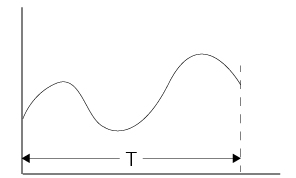
\includegraphics[width = 50mm, scale = 2]{Signal_1.jpg}
	 \caption{A random signal of width '$T$'}
	 \label{fig:signal1}
	 \end{figure}	 
	 Consider the signal shown in Figure \ref{fig:signal1}. This signal repeats after every interval of $T$ seconds. Now let us say we wish to express this signal as a linear combination of sine waves. As this signal has a time period of $T$, the very first component we must pick is a sine wave whose time period is $T$, that is, whose frequency $f_0 = \frac{1}{T}$. Evidently, a sine wave of frequency $f_0$ doesn't give us our signal back. We must add a few more sine waves. The next in the series of sine waves will be the one with time period $\frac{T}{2}$ or with frequency $2f_0$. However, we may still not have a linear combination of these two sine waves which gives us back our original signal. We then add a sine wave of time period $\frac{T}{3}$ or frequency $3f_0$. Once we continue this way, we see that to represent this signal, we must add all sine waves whose frequency is of the form $f = nf_0$, where $n = 1,2,3 \ldots$. However, this may still not give us our signal. If we observe closely, the \textit{average value} of our signal over the interval $T$, isn't zero. But if we average out our linear combination of sine waves, we will get zero! To correct this, we must also add a sine wave of \textit{zero} frequency. A constant. Finally, this gives us our original signal. Note that each component in our linear combination has an associated multiplying factor, or its \textit{``weight''}. This weight gives us the contribution of the corresponding sine wave to our signal. Thus, our signal can be represented as : 
	 \[x(t) = \sum_{i=0}^{\infty} (A_i \cos(2\pi if_0t) + B_i \sin(2\pi if_0t))\]
	 
	 where $A_i$ and $B_i$ are the coefficients associated with the sine wave having frequency $if_0$. This, is the \textbf{Fourier Series} of the given signal. We need two coefficients $A_i$ and $B_i$ to represent our signal. This is because we also need to account for the \textit{phases} of our sine waves. In simpler terms, we need to make sure that our linear combination and original signal have the same reference for $t=0$. This can be done by translation of our cosines forward or backward by a certain amount. This is exactly what's being done by the sine. However, this is a cumbersome notation. Using elementary trigonometric identities, we can represent this in a much neater manner as follows : 
	 \[
	 x(t) = \sum_{i=0}^{\infty} A_i \cos(2\pi if_0t + \phi_i)
	 \]
	 where $A_i$ is the weight of the frequency $if_0$ and $\phi_i$ represents the relative phase of the frequency $if_0$. We shall be using this notation henceforth. \smallskip
	 
	 The above representation is indeed, nice. But the signal we have picked here is also a particularly \textit{`nice'} signal. It doesn't have any discontinuities and is infinitely differentiable everywhere. But what about signals having discontinuities at certain points. As we saw, the Dirichlet conditions still allow us to to express such signals in terms of sine waves. But any linear combination of sine waves would be continuous and in fact, infinitely differentiable. How, then, can this linear combination be equal to our original, discontinuous signal. The idea is that here we relax our definition of \textit{convergence}. Even for such signals, the linear combination of sine waves converges at all points where the function is continuous, and at the points of discontinuity, it converges to a value which is the \textit{average} of the values at the two endpoints. Such a linear combination still largely retains the properties of the signals and we say that it converges `almost everywhere' to the original signal. As long as the points of discontinuity are isolated, they won't cause us much trouble. \smallskip
	 
	 Here, we introduce the concept of a frequency axis. A nice way to represent the set of coefficients $A_i$ is to consider the frequency to be our variable of interest, i.e, we shall have a mapping between the sets of frequencies $nf_0$ and the sets of coefficients $A_i$. We could then represent this mapping graphically in the \textit{frequency domain}. Our x-axis represents frequency and y-axis represents the weights or coefficients associated with these frequencies. At the points $x= if_0$, the y co-ordinate is equal to $A_i$. A similar plot can also be drawn for the coefficients $\phi_i$. 
	 
	 \subsection{From Periodic to Aperiodic : The Fourier Transform}
	 So far, we have only considered a \textit{periodic} signal. But what if our signal was aperiodic? How would we then represent it as a linear combination of sine waves? A nice way to do this is as follows: 
	 Consider that in Figure \ref{fig:signal1}, we make $T$ larger and larger. The gap between consecutive frequencies $\Delta = \frac{1}{T}$ would become smaller and smaller. To represent an aperiodic signal, we need $T \rightarrow \infty$ and consequently, $\Delta \rightarrow 0$. Hence, from a countably infinite set of frequencies, we reach a continuum of frequencies. The associated summation is then replaced by an integral. The sequences $A_i$ and $\phi_i$ become functions $A(f)$ and $\phi(f)$. Thus, our signal can be represented as : 
	 \[x(t) = \int_{0}^{\infty} A(f) \cdot \cos(2\pi ft+\phi(f)) df \]
	 The `amplitude' function $A(f)$ is commonly known as the \textbf{Fourier Transform} of $x(t)$. The above equation represents the \textbf{Inverse Fourier Transform} of $A(f)$ (or the representation of $x(t)$ in terms of sinusoids. 
	 
	\subsection{Why Sine Waves?}	 
	 Before we move onto Sampling, I would like to make a few points about \textit{why} we chose the sinusoids as our building blocks. An important point to note is that sinusoids behave the same way regardless of their frequencies. Thus our treatment of one sinusoid applies equally well to \textit{all} sinusoids. This is what makes the decomposition into sinusoids so powerful. We can treat every unit the same way and hence it is sufficient to analyse only one of them. In  contrast, consider the Taylor series. Here, the units are \textit{polynomials} in $x$. These most certainly do not behave in the same way. If we have treated $x$ in one way, we still have to treat $x^2$ in a completely different way, making our search for units pointless. The fact that we can expect similar results from the same operation on each sinusoid is what makes the sinusoids a powerful foundation for us. \smallskip
	 
	 Taking a bit of inspiration from linear algebra, what we have essentially done is an \textbf{orthogonal decomposition} of our signal. If we take the set of cosines to be our basis, then we have simply represented our signal as a linear combination of the basis elements. Particularly, the interesting property is that the set of cosines form an \textit{orthogonal} basis. That is the \textit{inner product} of any two cosines is zero if their frequencies are distinct and non-zero only when their frequencies are equal. Additionally, we could also \textit{normalise} this set of cosines to make the non-zero inner product equal to 1. This way, we end up with a peculiar factor of $\frac{1}{\sqrt{2\pi}}$ in our Fourier transform. The important point to note here is that orthogonality makes it extremely easy for us to find the coefficients $A_i$ and $B_i$ for a signal. All we need to do to is take the inner product of our signal (and hence, our linear combination) with the sine and cosine of our frequency of interest. This would make all inner-products equal to zero except for the sine/cosine of this frequency (this becomes 1 if our basis is normalised). Hence, this gives us the coefficient corresponding to this frequency. Thus, the Fourier transform is especially easy to compute.
	 \bigskip
	 
	 \section{Sampling}
	 \subsection{What exactly is Sampling?}
	 Now that we have a good idea about representing signals, we move on to the process of \textbf{sampling}. The process of sampling is a \textit{bridge} between the domains of continuous-time signals and discrete-time signals. When we sample a signal, what we are essentially doing is capturing the value of the signal at particular instants only, and reconstructing the original signal from these samples. An example where sampling is used is audio recordings. Sound is produced as continuous waveforms. However, the storage of these waveforms as continuous signals takes up too much space. This is where sampling comes in. In audio recordings, we do not keep track of the audio signal at all times. Instead, we only sample it at regular instants and store only these samples. We then use these set of samples to reconstruct the original sound waveform. In a sense, we have discretised sound. If we have a continuous-time signal $x(t)$, its sampled signal would be the value of the continuous-time signal at particular instants (sampling instants) and zero everywhere else. Thus a sampled signal is essentially a train of pulses. However this is the picture of only \textit{idealised} sampling. In reality, we cannot take pin-point snapshots in time and our snapshots tend to smear a bit about the sampling instants. Figure \ref{fig: sample1} depicts a more realistic picture of what sampling looks like.

	\begin{figure}[H]
	\centering 
	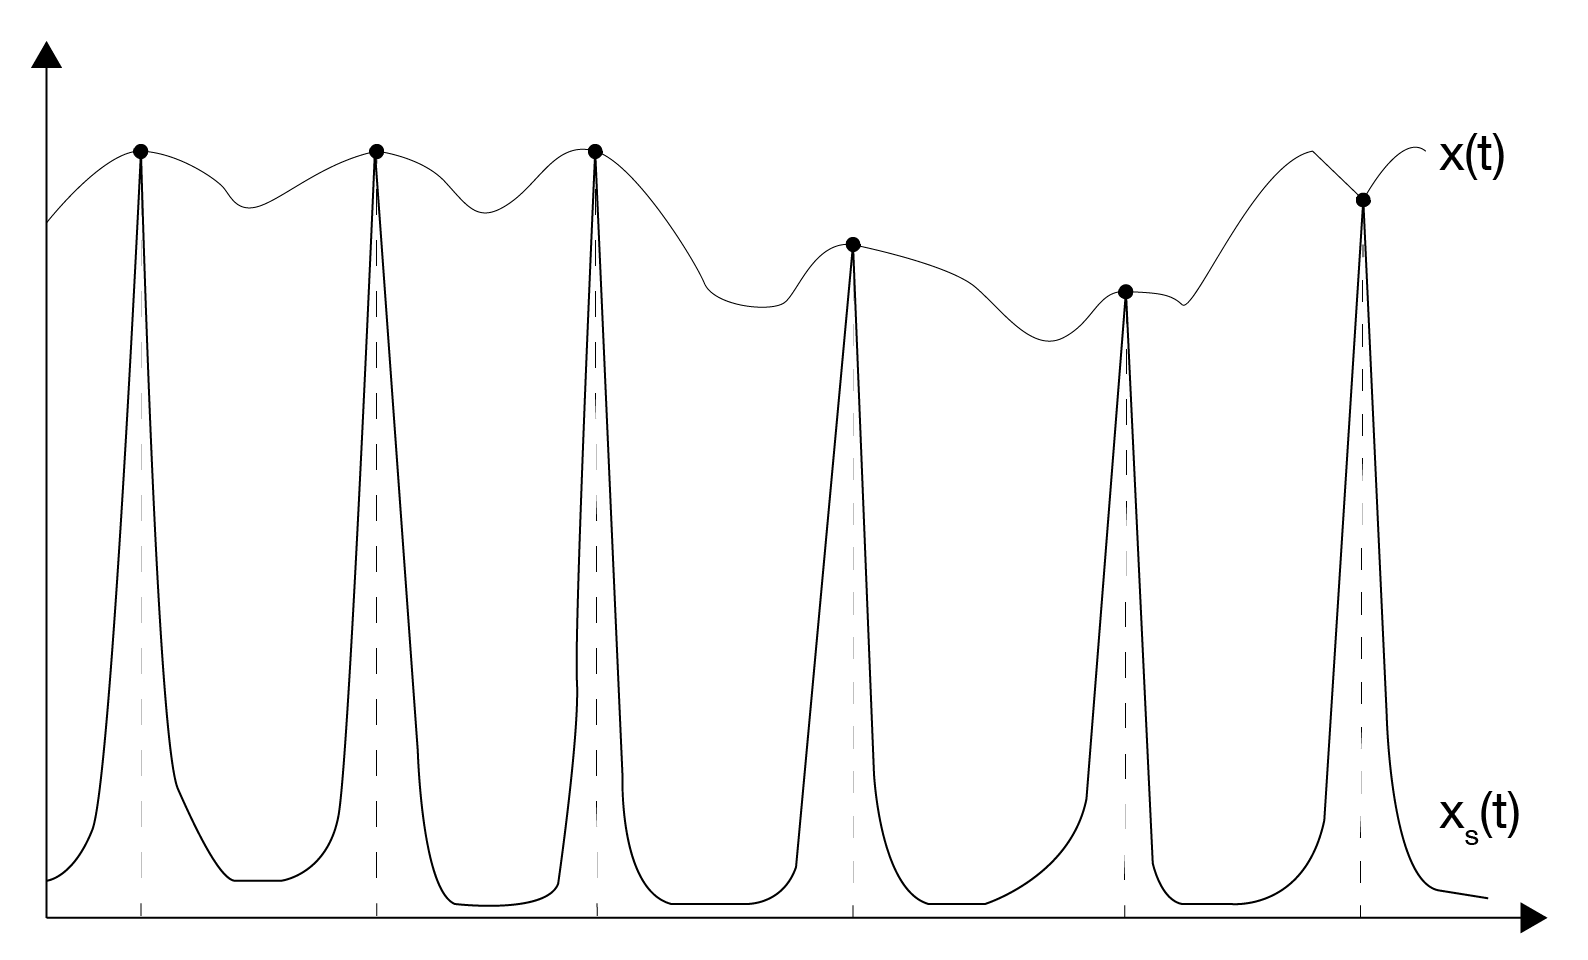
\includegraphics[scale=0.85]{Samples.png}
	\caption{Figure 2: A realistic picture of sampling}
	\label{fig: sample1}
	\end{figure}
	 Our objective is to recreate the signal, or obtain $x(t)$ from $x_s(t)$. It is not intuitive at this point that we can actually be able to do this. How is it that we only know the value of our signal at a few points yet we are able to completely describe it? And if it is indeed possible to carry out this process, how often must one know the value of our signal to exactly reconstruct it? Before we answer these questions, let us first talk a bit about the process of sampling.
	 
	 \subsection{More about sampling and the Nyquist Principle}
	 I would like to point out that sampling is a \textit{linear} process. Let's say I have two signals $x_1(t)$ and $x_2(t)$. When I sample these two signals separately, I get the samples $y_1[n]$ and $y_2[n]$ (where n is the sampling number, as shall be explained later). Now lets say I wish to sample a linear combination $\alpha_1 x_1(t) + \alpha_2 x_2(t)$ of the original signals. The corresponding samples I will get for this linear combination will be $\alpha_1 y_1[n] + \alpha_2 y_2[n]$. This is fairly intuitive as our signals themselves obey the law of \textit{superposition}. We shall exploit this linearity by invoking the Fourier representation of a signal. In the previous chapter, we saw that any signal could be broken down as a sum of 'shifted' cosines. Thus, to focus on sampling any general signal, we focus on the sampling of a single sine wave. \smallskip
	 
	Consider the sinusoid $x(t) = A\cos(2\pi ft + \phi)$. We wish to sample this signal and eventually reconstruct it from these samples. Consider that we sample this is signal at regular intervals of $T_s$. In this case, $T_s$ is the sampling interval and $f_s = \nicefrac{1}{T_s}$ is the sampling frequency. Our samples will be the value of $x(t)$ at the instants $t = nT_s$ for $n \in \mathbb{W}$. Here $n$ is the \textit{sampling number}, which tells us which sample are we currently looking at. Thus, our samples are :  
	\[
		y[n] = A\cos(2\pi f nT_s + \phi)
	\]
	
	Now our objective is this : given these samples, can we obtain the signal $x(t) = A\cos(2\pi ft + \phi)$ ? And if so, when? At first, it may seem that the problem with the sampling is that we cannot find a function which satisfies these samples. However, this is not true. The problem is that we have \textit{too many} functions which can satisfy these samples. For example, consider the samples $y[n] = A\cos(2\pi f n T_s + \phi)$ It is definitely not certain that these samples came from the signal $x(t) = A\cos(2\pi ft + \phi)$. We could very well choose our function to be made up of the line segments connecting two consecutive samples. This function could've also led to these samples, with equal merit. But we wish to talk about only sinusoids (as we are interested only in samples from sinusoids, having decomposed signals in terms of sinusoids). The problem is that even when we restrict ourselves \textit{only} to sinusoids, there are still many sinusoids which will satisfy these samples and in fact, infinitely many such sinusoids. This poses a big problem. For any set of samples, we have infinitely many sinusoids which may have produced them. How do we know which is the \textit{correct} sinusoid? This is the objective of reconstruction.  \smallskip
	
	To treat this problem of many sinusoids, we must first have an idea about why this non-uniqueness arises. Quite remarkably, this non-uniqueness arises because of the following two elementary trigonometric identities :
	
	\[ 
		\cos(\beta) = \cos(-\beta)
	\]  
	\[
		\cos(2\pi k + \beta) = \cos(\beta) \; \forall\:  k \in \mathbb{I}
	\]
	
	Thus, we can alternatively express represent $\cos(\beta)$ as $\cos(2\pi k \pm \beta)$ for all integer $k$, thus creating infinite possible representations of the same cosine. Now let us apply this to our samples. Our samples can be thus be represented as
	\[ 
		y[n] = A\cos(2\pi fnT_s + \phi) = A\cos(2\pi kn \pm 2\pi nfT_s \pm \phi)
	\]
	
	This can be further simplified to : 
	
	\[
		y[n]  = A\cos(2\pi nT_s ( \frac{k}{T_s} \pm f ) \pm \phi) = A\cos(2\pi nT_s (kf_s \pm f) \pm \phi)
	\]
	
	This representation says a lot! By separating out $2\pi nT_s$, we have found out the frequencies of the misleading sinusoids. For example, the samples could've been produced by the sinusoid having frequency $f_s + f$ and phase $+ \phi$ as well as by the sinusoid having frequency $f_s - f$ and phase $- \phi$ (for $k=1$). Or perhaps the sinusoid with frequency $2f_s+f$ and phase $+ \phi$ or the sinusoid with frequency $2f_s - f$ and phase $- \phi$ (for $k=2$). Thus, we have generated all the sinusoids which could've produced our samples. This can be explained as follows : in the expression $y[n] = A\cos(2\pi nT_s(kf_s \pm f) \pm \phi)$, $k$ represents the \textit{number of cycles lost} by the sinusoid before reaching our sample point. That is, the sinusoid with frequency $f_s + f$ completes one cycle before it reaches our sample point, while the sinusoid with frequency $2f_s + f$ completes two cycles before it reaches our sample point. Unsurprisingly, the sinusoids with higher $k$, have a higher frequency and thus complete a larger number of cycles between two sampling instants. Now, the sign of the phase tells us whether the sinusoid in question reaches our sampling point at its rising edge or falling edge. The sinusoids having same phase (i.e $+ \phi$) as our original signal pass through the sampling point on the same edge as the original sinusoid, while the sinusoids having opposite phase (i.e $- \phi$) pass through the sampling point on the opposite edge. \smallskip
	
	This process of creation of multiple copies of sinusoids producing the same samples is known as \textbf{Aliasing} and the copies of sinusoids produced are called \textbf{aliases}. The term `alias' refers to a false identity or a false persona. It is thus fitting to label these copies of sinusoids as aliases. The sinusoids with higher frequencies put on a false identity and masquerade as our original sinusoid by producing the same samples as the original signal. If we were to plot all these frequencies on the frequency axis, then we will have points corresponding to the frequencies : $f, f_s-f, f_s+f, 2f_s-f, 2f_s+f \ldots$. \smallskip
	
	We see that these aliases cause us a problem. Right now, we cannot tell which is the correct sinusoid. The discrete-time version of our signals (namely, the samples) has infinitely many continuous-time identities (namely, the aliases). What our process of reconstruction must do is filter out these aliases and pick the sinusoid of the correct frequency. \smallskip
	
	First, we consider the definition of a \textit{band-limited} signal. A band-limited signal is once whose component frequencies are bounded above, i.e, a band-limited signal has no contribution from frequencies higher than a certain frequency $f_m$ (the amplitude of its Fourier transform is zero for all frequencies greater than $f_m$). $f_m$ is the maximum frequency present in the signal. We now consider aliases of this band-limited signal. Our band-limited signal has frequencies in the range $0$ to $f_m$. This is called the \textit{spectrum} of our band-limited signal. Aliasing will simply copy and paste this spectrum at all multiples of $f_s$ and also paste this spectrum in reverse (or mirror it) at all multiples of $f_s$. Thus, the first alias of our band-limited signal will occupy the spectrum $f_s - f_m$ to $f_s$. The second alias will occupy the spectrum $f_s$ to $f_s + f_m$. The third will occupy the spectrum $2f_s - f_m$ to $2f_s$ and so on. If we are to ensure that we can reconstruct our signal from the samples, we must ensure that none of the aliases interfere with our original spectrum, i.e, the aliases do not \textit{pollute} our original spectrum. For this to hold true, there should be no overlap of the original spectrum with any of the alias spectra. Evidently, our trouble is restricted to only the \textit{first} alias. Once we have made sure that the first alias doesn't interfere with our signal, we have made sure that none of the aliases will. This is because all other aliases occupy bands which are farther away from our original spectrum. The minimum frequency contained in the spectrum of the first alias is $f_s - f_m$. To make sure that this spectrum doesn't overlap with our original spectrum, we must have that the point corresponding to the frequency $f_s - f_m$ lies to the right of the point corresponding to the frequency $f_m$ in our original spectrum. Thus we get that $f_s - f_m \geq f_m$, or :
	\begin{theorem}
				\[ \boxed{f_s \geq 2f_m} \] 
	\end{theorem}

		
		This important result is known as the \textbf{Nyquist Principle} or the \textbf{Nyquist-Shannon Sampling Theorem}. This equation gives us the criterion we have been looking for. This is \textit{not} a formal proof of the Nyquist principle, rather a simple and intuitive explanation for the same. However, we can add rigour to this very idea to formally prove the Nyquist principle. \smallskip 
		
		Let us now talk about a few points about what the Nyquist principle really tells us. The Nyquist principle tells us is that if my sampling frequency is greater than or equal to twice the maximum frequency present in my signal, then I can successfully reconstruct my signal from the samples taken. Note that the Nyquist principle does \textbf{not} tell us that aliases won't be created if $f_s \geq 2f_m$. Aliases will still be created. What this principle tells us is that even though these aliases are created, they won't pollute our original spectrum if our sampling satisfies the Nyquist criterion. In other words, once we have ensured that $f_s \geq 2f_m$, we have ensured that there is no intruder in our original spectrum, i.e, our original spectrum has not been distorted by aliases. It is now easy to see that we can obtain the true signal by keeping with us only the frequencies upto $f_m$. As the spectrum upto $f_m$ is the true spectrum of our signal, filtering out all frequencies above $f_m$ will give us back our true signal. This can be easily done with the help of a \textbf{Low Pass Filter}. \smallskip
		
		The Nyquist principle basically tells us that to successfully reconstruct our signal, we must sample it atleast twice per cycle. But, it is also possible that we may not be able to reconstruct our signal if we sample it \textit{exactly} two times. For example, consider the sinusoid $x(t) = A\cos(2\pi ft)$. Consider that we sample this signal at all the points $t = \frac{n}{2f}$ for integer n. We still have exactly two samples per cycle but all our samples turn out to be zero! We have lost all information about our signal simply because we sampled it at the wrong instants. This problem only arises for the case $f_s = 2f_m$ (or the \textit{perfect sampling} case). This won't happen if we sample it at a frequency $f_s > 2f_m$. Hence, it is always safer to sample at a frequency sufficiently higher than $2f_m$. For example, audio signals (which have a maximum frequency of $20$ kHz) are usually sampled at $44$ kHz, which is an  entire $4$ kHz higher than the minimum sampling frequency provided by the Nyquist principle. Before we move on, let us consider an interesting effect of incorrect sampling, which arises due to aliasing. 
		
		\subsection{The Wagon Wheel Effect}
		
		How often have we observed wheels turning backwards in films? This can actually be elegantly explained by aliasing. The films we view are actually a rapid display of separate images (or frames). Most films have a rate of $24$ fps (frames per second). These frames are basically our samples and $24$ fps is our sampling rate. The Nyquist principle tells us that the alias spectrum will overlap with the true spectrum if the maximum frequency is greater than $\frac{f_s}{2}$ or $12$ fps. Thus, we'll be able to see the negative effects of aliasing if there are any transitions in our film which are faster than $12$ fps. This is commonly seen in rotating wheels.  \smallskip
		
		Consider a wheel with $8$ spokes. Now, let's say that the wheel is rotating at $2$ revolutions per second. Now, the number of spokes it'll move forward by in one second will be given as :
		
		\[ \frac{2(\text{rps}) \times 8(\text{spokes/revolution})}{24 \text{fps}} = 0.67 \text{spokes/frame} \]
		
		Thus, in one frame, the wheel moves forward by approximately $67$ \% of the angular distance between two spokes. However, when viewing these two frames consecutively, this is perceived by the human eye as the wheel moving \textit{backward} by $33$ \%. Thus, we get the illusion that the wheel is actually moving backward. The apparent speed of the backward motion can also be calculated as follows : 

\[ 
	\omega_{\text{apparent}} = \frac{24 \text{fps} \times 0.33 (\text{spokes/frame})}{8 (\text{spokes/revolution})} = 1 \text{rps} 
\]	

Thus, the wheel actually appears to move backward with a speed of $1$ rps. The Nyquist principle gives us a really nice explanation for this phenomenon. If in two successive frames, the spokes move by more than $50$ \% of the angular distance, it actually appears to us as if the \textit{next} spoke has moved backward. To resolve this, we must make sure that we sample fast enough so that the angular distance covered in two consecutive frames is less than $50$ \% of the total angular distance between two spokes. This again leads us back to the Nyquist principle. Hence, in the problem above, if the wheels rotate at a speed \textit{less than} $1.5$ rps, we will not face this problem of the wheels moving backward (as the spokes cover less than $50$ \% of the angular distance as can be easily calculated). An interesting thing happens if we make the wheels rotate at $3$ rps. The percentage of angular distance covered will thus be :

\[ 
	\frac{3(\text{rps}) \times 8(\text{spokes/revolution})}{24 \text{fps}} = 1 \text{spoke/frame}
\]
		
		This is a \textit{really} interesting result. In one frame, each spoke covers \textit{$100$ \%} of the angular distance. Thus, each spoke moves to the position of the next one. However, our eyes cannot tell apart one spoke from another. Hence what appears is that the wheel actually remains \textit{stationary}. This is quite uncommon though as we need to be quite lucky to hit this sweet spot.
		
		\subsection{Introducing Complex Exponentials and Phasors}
		
		We have now analysed sampling in a fair amount of depth. Before we proceed further, I would like to introduce some ideas about the representation of sinusoids themselves. Consider our good old sinusoid $A\cos(\omega t + \phi)$. We will often see that most systems modify this sinusoid in a combination of the following two ways :
		
		\begin{enumerate}
		\item Modifying the amplitude 
		\item Modifying the phase
		\end{enumerate}
		
		Let us first consider modifying the amplitude only. Our sinusoid $A\cos(\omega t + \phi)$ is transformed into the new sinusoid $A_1 \cos(\omega t + \phi)$. This new sinusoid can also be represented as: 
		
		\[A_1\cos(\omega t + \phi) = \frac{A_1}{A} \times A\cos(\omega t + \phi) \]
		
		Thus, an amplitude change is simply performed by the multiplication of the factor $\frac{A_1}{A}$. This is a convenient way to represent amplitude changes. Now we consider modifying the phase only. Our sinusoid $A\cos(\omega t + \phi)$ is transformed into the sinusoid $A\cos(\omega t + \phi_1)$. But, when we look for an analogous multiplication factor, we run into trouble. It isn't possible for us to simply multiply the sinusoid $A\cos(\omega t + \phi)$ with a constant and get the sinusoid $A\cos(\omega t + \phi_1)$. This makes it very inconvenient for us to handle phase changes in sinusoids. We now wish to replace the sine with a function that allows us to conveniently handle both phase changes and amplitude changes. Note: while making phase changes convenient to handle, we must still retain the convenience with amplitude changes. To do this, we move into the realm of \textit{complex numbers}. \smallskip
		
		Consider a complex number $z = Ae^{j(\omega t + \phi)}$ where $j$ is the square root of minus one ($j = \sqrt{-1}$). This is the \textit{polar form} of $z$. $z$ can also be represented in its \textit{rectangular form} as $z = A\cos(\omega t + \phi) + jA\sin(\omega t + \phi)$. The real and imaginary parts of $z$ are  $\Re(z) = A\cos(\omega t + \phi)$ and $\Im(z) = A\sin(\omega t + \phi)$.  respectively. We also consider the complex conjugate of $z$, $\bar{z} = Ae^{-j(\omega t + \phi)} = A\cos(\omega t + \phi) - jA\sin(\omega t + \phi)$. Now, when we average these two complex numbers, we get :
		
		\[ 
			\frac{1}{2}(z + \bar{z}) = \frac{Ae^{j(\omega t + \phi)} + Ae^{-j(\omega t + \phi)}}{2} = A\cos(\omega t + \phi)
		\]
		
		This is the representation of sinusoid we have been looking for, i.e, $A\cos(\omega t + \phi) = \frac{1}{2}(Ae^{j(\omega t + \phi)} + Ae^{-j(\omega t + \phi)})$. To give a bit of intuition, the complex exponential $Ae^{j(\omega t + \phi)}$ is the complex number of magnitude $A$, having initial phase $\phi$ and rotating with an angular speed of $\omega$ in the anticlockwise direction. Its complex conjugate is simply its mirror image, i.e, the complex number with magnitude $A$, having initial phase $-\phi$ and rotating with an angular speed of $\omega$ in the clockwise direction. The sinusoid $A\cos(\omega t + \phi)$ is then the average of the \textit{projections} of the two complex exponentials onto the real axis in the Argand plane. \smallskip
		
		Now let us see if our complex exponential gives us a multiplicative factor for phase change. Consider the complex exponential $Ae^{j(\omega t + \phi)}$. We wish to transform this into the complex exponential $Ae^{j(\omega t + \phi_1)}$. But, we can represent this new exponential as : 
		
		\[ 
			Ae^{j(\omega t + \phi_1)} = Ae^{j(\omega t + \phi)} \times e^{j(\phi_1 - \phi)}
		\]
		
		Thus we have represented a phase shift via multiplication. The factor $e^{j(\phi_1 - \phi)}$ is the multiplicative factor. The important point to note is that this representation \textit{still} allows us to represent amplitude changes by multiplication of the \textit{same} factor $\frac{A_1}{A}$. More conveniently, any arbitrary transformation from $Ae^{j(\omega t + \phi)}$ to $A_1e^{j(\omega t + \phi_1)}$ can be achieved by multiplying with the factor $\frac{A_1}{A} e^{j(\phi_1 - \phi)}$. Note: to represent the same change in the sinusoid $A\cos(\omega t + \phi)$, we must make changes to both the complex exponentials making up the sinusoid. While they have the same amplitude factor, their phase factors are mirror images of each other. For example, we saw that we must multiply the first complex exponential with the factor $e^{j(\phi_1 - \phi)}$, the second one must be multiplied by the factor $e^{-j(\phi_1 - \phi)}$. This ensures that the components still remain mirror images after the transformation. \smallskip
		
		
		Now that we have introduced this representation of sinusoids, we'll go one step further and introduce the concept of \textbf{phasors} (or \textbf{phase vectors}). We considered $A\cos(\omega t + \phi)$ to be the average of two rotating complex numbers, $Ae^{j(\omega t + \phi)}$ and $Ae^{-j(\omega t + \phi)}$. The phasor is simply the term $Ae^{j\phi}$ or $Ae^{-j\phi}$. These terms can also be considered as the \textit{complex amplitudes} associated with the frequencies $\omega$ and $-\omega$. We see that the concept of phasors also introduces us to \textit{negative} frequencies. A negative frequency simply means that the associated complex number is rotating in the clockwise (or negative) direction. The phasor $Ae^{j\phi}$ can also be represented as $A\angle\phi$. Using phasors, we can say that the sinusoid $A\cos(\omega t + \phi)$ is the average of the phasors $A\angle\phi$ and $A\angle -\phi$ associated with the frequencies $\omega$ and $-\omega$ respectively. For real signals, we see that the magnitude is an \textit{even} function of frequency and phase is an \textit{odd} function of frequency. Henceforth, we will consider signals to be combinations of phasors . 
		
		\subsection{Sampling with Phasors}
		
		We now look back at our problem of sampling using phasors. We consider the same signal, occupying a band between the frequencies $0$ to $f_m$. For each frequency $f$, we will have phasors created at the frequencies $f$ and $-f$. Thus, in terms of phasors, our signal occupies the spectrum from $-f_m$ to $f_m$. Aliasing will still occur the same way, but the only difference is that aliases will also be created for negative frequencies. For example, the alias corresponding to the frequency $f_s - f_m$ will be resolved into phasors associated with the two frequencies $f_s - f_m$ (positive) and $-f_s + f_m$ (negative). The rest of the treatment remains the same. 
		
		\subsection{Normalised Frequency}
		
		We now describe what is called the process of \textit{normalisation}. In normalisation, we change our units to make the sampling frequency as our unit angular frequency. This makes $f_s = 2\pi$. All other frequencies are now represented in terms of this \textit{new} unit. Our new notion of frequency (or normalised frequency) is defined as the ratio of the actual frequency to the sampling frequency. We use these normalised frequencies to construct a normalised frequency axis. The sampling frequency $f_s$ occupies the points $2\pi$ and $-2\pi$ (in phasors). If our signal obeys the Nyquist principle, then it occupies the spectrum $-\pi$ to $\pi$. The spectrum of our signal is unique \textit{only} in this region. This spectrum between $-\pi$ and $\pi$ is copied and pasted at all multiples of $2\pi$. These are the alias spectra. \smallskip
		
		We have described normalised frequencies, but why do we need them? Normalised frequency adds a sense of \textit{abstraction} to our process of sampling. The idea is that we want to use the same principle of sampling for any given sampling frequency. We don't want to treat sampling any differently for two different physical situations. Normalisation allows us to ignore the physical situation we are dealing with and allows us to treat these situations the same way. It allows us to use a common philosophy for all scenarios.
		\clearpage

\section{Discrete Systems and Linear Shift-Invariant Systems}

\subsection{What is a discrete system?}

After talking about sampling, we now move on to systems which process such samples or digital signals. These are called \textbf{discrete systems}. 
		
\begin{defn} A discrete system is one which takes in a sampled input and gives out a sampled output. Schematically :
		
		
\begin{tikzpicture}
  [scale=.8,auto=centre,every node/.style={circle,draw=black, fill=white!50}]
  \node (n1) at (1,10) {x[n]};
  \node (n2) at (10,10)  {Discrete System};
  \node (n3) at (19,10)  {y[n]};

    \draw[->] (n1) edge (n2) (n2) edge (n3);

\end{tikzpicture}
\end{defn}

Here $x[n]$ is our sampled input and $y[n]$ is our sampled output. The square brackets around $n$ indicate that this is a discrete signal or a \textit{sequence}. $n$ is the sampling number. Before we go on, it is interesting to note that there is some equivalence between a discrete system and an analog system having the same function. Consider that we send an input $x(t)$ through an analog system which gives us the output $y(t)$. The output $y(t)$ can also be obtained in this way : We first sample the input $x(t)$ according to the Nyquist principle to get the sampled input $x[n]$. We the pass this sampled input through an \textit{equivalent} discrete system which gives us the sampled output $y[n]$. Now, when we reconstruct the output signal from the samples $y[n]$, we get back the analog output $y(t)$. This can be depicted in a neat way as follows : \\

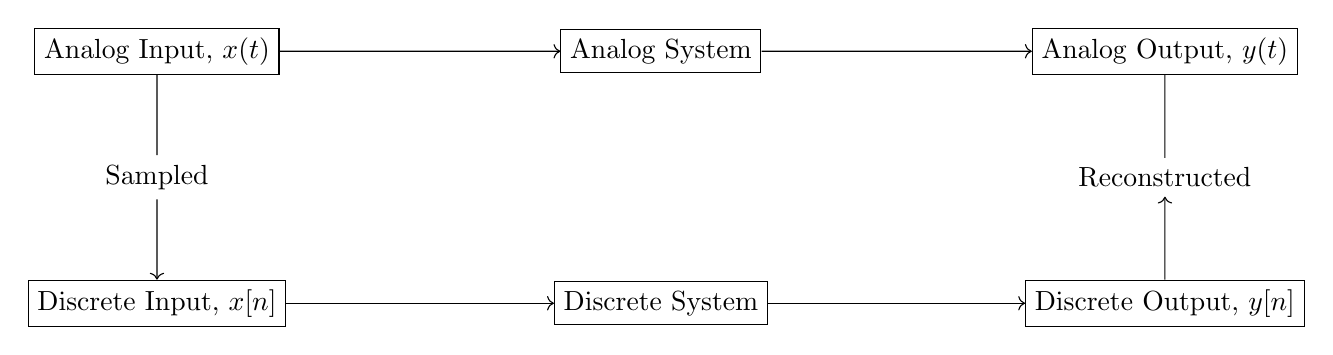
\begin{tikzpicture}
[scale = .8, auto = left]
\node[rectangle, draw=black, fill=white!20] (n1) at (1,4) {Analog Input, $x(t)$};
\node[rectangle, draw=black, fill=white!20] (n2) at (9,4) {Analog System};
\node[rectangle, draw=black, fill=white!20] (n3) at (17,4) {Analog Output, $y(t)$};
\node[rectangle, draw=black, fill=white!20] (n4) at (1,0) {Discrete Input, $x[n]$};
\node[rectangle, draw=black, fill=white!20] (n5) at (9,0) {Discrete System};
\node[rectangle, draw=black, fill=white!20] (n6) at (17,0) {Discrete Output, $y[n]$};
\node[rectangle, fill=white!20] (n7) at (1,2) {Sampled};
\node[rectangle, fill=white!20] (n8) at (17,2) {Reconstructed};

\draw[->] (n1) edge (n2) (n2) edge (n3) (n4) edge (n5) (n5) edge (n6) (n7) edge (n4) (n6) edge (n8);
\draw (n1) -- (n7);
\draw (n8) -- (n3);

\end{tikzpicture} \\

A discrete system is described by the relationship between $x[n]$ and $y[n]$. It can be considered as a mapping from one sequence to another. A sequence itself can itself be considered as a mapping from $\mathbb{Z} \rightarrow \mathbb{C}$. It takes in an integer $n$ (the sampling number) and gives a complex output. So a discrete system is a relation between two such sequences. Note that the relation need not be a direct correlation between $x[n]$ and $y[n]$, i.e $y[n]$ need not be related to $x[n]$. It can also be related to $x[n-1]$ or $x[n-2]$. It need not be a point-to-point relation either. It can also be related to multiple samples, such as $y[n] = x[n] + x[n-1]$. An example of this is a system which \textit{accumulates} its inputs. This will be defined as :

\[ 
	y[n] = \sum_{i=-\infty}^{n} x[i]
\]

A system in which $y[n]$ is related \textit{only} to $x[n]$ is called a \textbf{memoryless} system. This is because the system does not keep track of its previous inputs and is only connected to the \textit{current} input.


\subsection{Linearity}

Now that we have a good idea of what a discrete system is, we talk about what we require from discrete systems which are relevant to us. The basic requirement is that our system must treat frequencies independently. If we give our system an input phasor of certain frequency, our output must be a phasor of the \textit{same} frequency. This is important because when we take a combination of phasors and put it into our system, we must ensure that the action of our system on one frequency doesn't affect another frequency. For memoryless systems, it is easy to see that the only system which obeys these properties is the linear system $y[n] = k\times x[n]$ for some complex $k$. If we give it an input $x[n] = Ae^{j(\omega n + \phi)}$ we get the output $y[n] = k\times Ae^{j(\omega n + \phi)}$ which can be written as $A_1 e^{j(\omega n + \phi_1)}$ for some $A_1 , \phi_1$. Thus our output $y[n]$ also has the same frequency $\omega$. \smallskip

Consider however the system $y[n] = x^2[n]$. This is a non-linear system and does not obey our requirement. If we give it an input $x[n] = Ae^{j(\omega n + \phi)}$ we get the output $y[n] = A^2 e^{j(2\omega n + 2\phi)}$, which has double the frequency of our input. Essentially, we want our system to obey what is called the \textbf{principle of superposition}. The principle of superposition tells us that if I send two signals $x_1[n]$ and $x_2[n]$ through a system to get the outputs $y_1[n]$ and $y_2[n]$ respectively, then on sending a linear combination $\alpha x_1[n] + \beta x_2[n]$ through the system, I should get the output $\alpha y_1[n] + \beta y_2[n]$ corresponding to the \textit{same} linear combination $\alpha, \beta$. Mathematically, for any two sequences $x_1[n]$ and $x_2[n]$ :

\[
	f(x_1[n]) = y_1[n] , \: f(x_2[n]) = y_2[n] \implies f(\alpha x_1[n] + \beta x_2[n]) = \alpha y_1[n] + \beta y_2[n] , \: \forall \: \alpha, \beta \in \mathbb{C}.
\]

A system that obeys this property or obeys the principle of superposition is called a \textbf{linear system}. To illustrate certain properties about linearity, we take two examples. \smallskip

First, consider the system $y[n] = \Im(x[n])$, the imaginary part of $x[n]$. Although this system appears to be linear at first, it actually isn't. The problem arises when we consider \textit{complex} constants while taking linear combinations. For example, consider $x_1[n] = 1$ and $x_2[n] = 1$, two constant sequences. Now, $y_1[n] = 0$ and $y_2[n] = 0$. Consider, however the linear combination $x[n] = x_1[n] + jx_2[n] = 1 + j$, with the coefficients $\alpha = 1, \beta = j$ ( $j = \sqrt{-1}$). Output obtained is $y[n] = \Im(1+j) = 1$, while $\alpha y_1[n] + \beta y_2[n] = 0$. Clearly, $y[n] \neq \alpha y_1[n] + \beta y_2[n]$. Hence, this system isn't linear. An interesting property to note is that although the system isn't linear, it obeys the principle of superposition when we restrict ourselves to only taking the \textit{sum} of any two signals. Indeed, $\Im(x_1[n] + x_2[n]) = \Im(x_1[n]) + \Im(x_2[n])$. This property of a system is called \textbf{additivity}. Thus, the system $y[n] = \Im(x[n])$ is an additive system. \smallskip

Coming to our second example, consider the following system : 

\[
	 	y[n] = 
	 	\begin{dcases}
        \frac{x^2[n]}{x[n-1]} & \emph{if} \ x[n-1] \neq 0 \\
        0 & \emph{otherwise.} \\
   		\end{dcases}
	 \]
	 
	 It is easy to see that this system is non-linear. However, this system also has a special property. Although this system isn't linear, it obeys the principle of superposition when we restrict ourselves to only \textit{multiplying} the signal by a complex constant. Indeed if $x[n]$ gives the output $y[n]$, then the input $\alpha x[n]$ gives the output $\alpha y[n] \; \forall \: \alpha \in \mathbb{C}$. This property of the system is called \textbf{homogeneity}. Thus, the given system is a homogeneous system. \smallskip
	 
	 These properties of additivity and homogeneity define linearity. A system is linear if it is both homogeneous and additive. This can be neatly explained as follows. A mapping from $y_1[n]$ , $y_2[n]$ to $\alpha y_1[n] + \beta y_2[n]$ is guaranteed only if $y_1[n]$ is mapped to $\alpha y_1[n]$, $y_2[n]$ to $\beta y_2[n]$ and if $\alpha y_1[n]$ , $\beta y_2[n]$ are mapped to $\alpha y_1[n] + \beta y_2[n]$ when we perform the corresponding operations on the inputs $x_1[n]$ , $x_2[n]$. By definition, homogeneity guarantees the first two mappings and additivity guarantees the third. Hence additivity and homogeneity together guarantee linearity, or a linear system is one which is both additive and homogeneous. 

\begin{defn}	 
	 A linear system can thus also be defined as one which obeys the following two properties : 
	 
	 \begin{enumerate}
	 \item For all inputs $x[n]$, if the output of $x[n]$ is $y[n]$, then the output of $\alpha x[n]$ must be $\alpha y[n] \: \forall \; \alpha \in \mathbb{C}$.
	 \item For any two inputs $x_1[n]$ , $x_2[n]$, if the corresponding outputs are $y_1[n]$ , $y_2[n]$, then the output of $x_1[n] + x_2[n]$ must be $y_1[n] + y_2[n]$.
	 \end{enumerate}
	 
	 \end{defn}
	 
	 The important question to ask at this point is : \textit{Is linearity enough to meet our criterion?} And the answer is no. Linearity is a necessary, but not a sufficient condition, as shall be shown ahead.
	 
	 \subsection{Shift Invariance}
	 
	 Apart from linearity, another important property of systems is \textbf{Shift Invariance}. What this basically means is that our system must react in the same way to a particular input $x[n]$ even if that input was sent at a different time. This can be defined as follows :
	 
	 \begin{defn}
	 A system is defined as a shift-invariant system if it satisfies the following property : 
	 
	 If a particular input $x[n]$ gives the output $y[n]$, then the input $x[n+d]$ must give the output $y[n+d]$, for any input sequence $x[n]$ and any $d \in \mathbb{Z}$.
	 \end{defn}
	 
	 In other words, if we shift our input sequence by any arbitrary number of samples, then the corresponding output sequence must be shifted in the same way. This must hold for all input sequences. Shift invariance is important as it ensures that our system obeys the same characteristics throughout time. Shift invariance is also an essential property we require in systems to ensure that a complex exponential input produces a complex exponential output. To illustrate this, consider the system $y[n] = n x[n]$. Clearly, this system is linear. But, it doesn't obey our property. When we send in the input phasor $x[n] = A_0 e^{(\omega_0 n + \phi_0)}$, we get the output $y[n] = A_0 n e^{(\omega_0 n + \phi_0)}$, which isn't a phasor, as the amplitude of $y[n]$ varies with $n$. The source of this error is the fact that the same input produces different outputs based on when it is sent into the system. This very problem is solved by shift invariance. \smallskip
	 Note : Shift Invariance is the more general "version" of the more common 'Time Invariance'. Time Invariance is Shift Invariance in which the independent variable is time. The question to ask now is : Are linearity and shift invariance sufficient conditions for our system to meet our objective. Before answering this question, we talk about certain properties of Linear Shift Invariant (LSI) Systems, and find a way to characterise LSI systems through what is known as the \textbf{unit impulse response} of an LSI system.
	 
	 \subsection{Unit Impulse Response and Convolution}
	 
	 The \textbf{unit impulse} is the signal $x[n]$ which is equal to $1$ for $n=0$ and equal to $0$ for all $n \neq 0$. The unit impulse signal is represented as $\delta[n]$. The signal $\delta[n]$ is the unit impulse signal centred at $n=0$. However, we can also construct a signal which is $1$ at an arbitrary point $n=n_0$ and zero everywhere else. Such a signal would be represented as $\delta[n-n_0]$. The signal which is $2$ when $n=0$ and zero everywhere else would be represented as $2 \times \delta[n]$. \smallskip
	 
	 The unit impulse response of an LSI system is the output sequence $y[n]$ when the input sequence is the unit impulse ($x[n] = \delta[n]$). The unit impulse response of an LSI system is commonly denoted by $h[n]$. For example, consider the system $y[n] = x[n] + x[n-1]$. Its unit impulse response will be $h[n] = \delta[n] + \delta[n-1]$. Thus, we get the unit impulse response as $h[n]$, which is equal to $1$ when $n=0$ or $n=1$ and equal to zero otherwise. \smallskip
	 
	 Before illustrating the power of the unit impulse response, we first show an interesting feature of the unit impulse signal. Any input sequence $x[n]$ can be represented as a linear combination of appropriately scaled and shifted unit impulses. This is fairly straightforward to see. For the index $i$, we construct $x[i]$ by multiplying $x[i]$ to the unit impulse at that index, or $\delta[n-i]$. On adding up these terms for all integer $i$, we get back our original sequence $x[n]$. Thus $x[n]$ can be represented as follows : 
	 
	 \[
	 		x[n] = \sum_{i=- \infty}^{\infty} x[i] \cdot \delta[n-i]
	 \]
	 
	 To verify this, consider that we put $n=k$. In the summation, all the $\delta$ terms not corresponding to $i=k$ vanish as the unit impulse function is zero there. What remains is simply $\delta[k-k] = 1$. This is then scaled by $x[k]$. Hence, we obtain our original sequence, as we can do this for every $k$. This notation seems a bit more cumbersome than the convenient notation $x[n]$. But this is a really powerful tool as it enables us to construct the output sequence $y[n]$ via the unit impulse response $h[n]$. \smallskip
	 
	 We start with the input sequence $\delta[n]$. This produces the output $h[n]$, the unit impulse response of our LSI system. We now shift our input by $'k'$ samples. As our system is shift invariant, the output will also shift by $'k'$ samples. Thus we now get the input-output pair $\delta[n-k]$ , $h[n-k]$. We now multiply our input by the constant $x[k]$, the value of our input at $n=k$. As our system is homogeneous, the output is also multiplied by the same constant. So, we get the input-output pair $x[k]\cdot \delta[n-k]$ , $x[k] \cdot h[n-k]$. Finally, we invoke additivity, and sum over all integer $k$. Hence finally, our LSI system takes in $\sum_{k=-\infty}^{\infty} x[k] \cdot \delta[n-k]$ as our input and gives the output $\sum_{k=-\infty}^{\infty} x[k] \cdot h[n-k]$. Now, note that the input is simply $x[n]$, as was shown above. Therefore, the output is our required output sequence $y[n]$. Thus, we can write : 
	 
	 \[
	 	\boxed{y[n] = \sum_{k=-\infty}^{\infty} x[k]\cdot h[n-k]}
	 \]
	 
	 This was possible only because our system was linear and shift-invariant. Hence, we state the following important theorem:
	 
	 \begin{theorem}
	 The output of any input sequence is known for an LSI system if we know its impulse response. In other words, An LSI system is completely characterised by its impulse response.
\end{theorem}	  

The output $y[n]$ is obtained by performing a certain operation between the two sequences $x[n]$ and $h[n]$. This operation proves to be really important in the field of signal processing. It is known as \textbf{Convolution}. In the equation $y[n] = \sum_{k \in \mathbb{Z}} x[k] \cdot h[n-k]$, we say that $x[n]$ and $h[n]$ are \textit{convolved} to obtain $y[n]$ or $y[n]$ is obtained from the \textit{convolution} of $x[n]$ and $h[n]$. Convolution is not an operation which is restricted only to an input sequence and the impulse response. Convolution can be performed on any two sequences. \smallskip

It is recommended that the reader try out this operation of convolution by hand on two \textit{finite-length} sequences to get a better understanding of convolution. Finite-length sequences are sequences which are non-zero only at finite instances. On working, it is easy to verify the following proposition.

\begin{prop}
The maximum possible number of non-zero points in the convolution, $y[n]$, of $x[n]$ and $y[n]$ is equal to one less than the sum of number of non-zero points in $x[n]$ and $h[n]$.

Or : $(N_{y[n]})_{max} = N_{x[n]} + N_{h[n]} - 1$, where $N_{\alpha[n]}$ denotes the number of non-zero points in the sequence $\alpha[n]$
\end{prop}

A detailed proof of this is left as an exercise to the interested reader. To visualise this process of convolution, consider the following. $h[n-k]$ is simply the sequence $h[k]$ starting at the index $n$ and reversed. To obtain the convolution of $x[n]$ and $h[n]$, we first fix a particular $n$. We centre the reverse sequence $h[-k]$ at this $n$. Then we take the product of $x[k]$ and $h[n-k]$ at corresponding locations and sum up all these products. This gives us the value for the convolution at a particular $n$. We repeat this process for all $n$, to obtain our convolved sequence $y[n]$. The process of convolution can be represented in a concise manner as follows : \smallskip

If $y[n]$ is the convolution of $x[n]$ and $h[n]$, we can denote $y[n]$ as : $y[n] = x[n] * h[n]$. It is clear that the convolution of two sequences may not always be defined. The sum $x[n] * h[n]$ is an infinite sum for every instance of the convolution. For the convolution to be defined, this sum must be convergent at every value of $n$. Evidently, it is possible that the sum may be divergent. Consider $x[n]$ and $h[n]$ to be two constant sequences having value $1$ at all points. Clearly, the convolution summation $y[n] = \sum_{k \in \mathbb{Z}} x[k] \cdot h[n-k] = \sum_{k \in \mathbb{Z}} (1)$ is divergent.

Now we prove two rather simple but powerful results, namely, the \textit{commutativity and associativity of convolution}. First, lets prove commutativity.
\begin{proof}
Consider the convolution 

\[
	y[n] = \sum_{k \in \mathbb{Z}} x[k]\cdot  h[n-k]
\]

Let us define $l = n-k$. $l = n-k \Rightarrow k = n-l$.


$k$ runs over all integers, $\mathbb{Z} \Rightarrow l$ runs over all integers, $\mathbb{Z}$.

\[
	\therefore y[n] = \sum_{l \in \mathbb{Z}} h[l] \cdot x[n-l] 
\]

This is the same expression as the first one, but with the roles of $x[n]$ and $h[n]$ interchanged. 
Hence, convolution is commutative, or $x[n] * h[n] = h[n] * x[n]$.
\end{proof}
Now, we prove associativity.
\begin{proof}
Consider that we convolve the convolution of two sequences $a[n]$ and $b[n]$ with a third sequence $c[n]$. 

\[
    (a[n] * b[n]) * c[n] = \sum{k \in \mathbb{Z}} (a*b)[n-k] \cdot c[k] = \sum_{k \in \mathbb{Z}} \sum_{l \in \mathbb{Z}} a[n-k-l] \cdot b[l] \cdot c[k]
\]
Now, we put $m=n-k-l$.
\[
    (a[n] * b[n])*c[n] = \sum_{k \in \mathbb{Z}} \sum_{m \in \mathbb{Z}} a[m] \cdot b[n-m-k] \cdot c[k] = a[n]*(b[n]*c[n]) 
\]
Hence, convolution is associative.
\end{proof}
Now, let us shift our focus back to the problem of input phasors and output phasors. We wish to check if linearity and shift invariance are sufficient conditions for our system to obey the requirement that an input phasor will give an output phasor of the same frequency. For any LSI system, the output sequence can be written as : 

\[
	y[n] = \sum_{k \in \mathbb{Z}} h[k]\cdot x[n-k]
\]

where $h[n]$ in the impulse response. Consider that we give in the input $x[n] = A_0 e^{j(\omega_0 n + \phi_0)}$. The output will be given as :

\[
	y[n] = \sum_{k \in \mathbb{Z}} h[k]\cdot x[n-k] = \sum_{k \in \mathbb{Z}} h[k] \cdot A_0 e^{j(\omega_0 (n-k) + \phi_0)}
\]

\[
	\therefore \boxed{y[n] = \left(A_0 e^{j(\omega_0 n + \phi_0)}\right) \times \sum_{k \in \mathbb{Z}} h[k] \cdot e^{-j\omega_0 k} }
\]

In the above expression, for a particular $\omega_0$, the term $\sum_{k \in \mathbb{Z}} h[k] \cdot \exp(-j\omega_0 k)$ will be a complex constant which will alter the phase and magnitude of the input $x[n]$. Hence the output $y[n]$ is also a phasor of the same frequency. Thus, we see that linearity and shift invariance are enough to satisfy our requirement. There is still one problem though. Our assertion holds true \textit{only} if the infinite sum converges. Thus, if the sum is convergent, our system satisfies our requirement. This introduces us to one more property necessary in our system - namely, \textbf{stability}.

\subsection{Stability and the Frequency Response} 

Before we talk about stability, we spend some time talking about the troublesome term $\sum_{k \in \mathbb{Z}} h[k] \cdot \exp(-j\omega_0 k)$. This term is a function only of the input frequency $\omega_0$. This term is denoted as $H(\omega_0)$ and, if convergent, is known as the \textbf{frequency response} of the system. $H(\omega_0)$ is a complex constant which alters the phase and magnitude of our input, to give us the output. Thus, we can represent the output as $y[n] = x[n] \times H(\omega_0)$, when $x[n]$ is an input phasor of frequency $\omega_o$. It is important to note here that we are dealing with normalised frequencies, as was decided earlier. The frequency response may or may not be defined, depending on the convergence of the infinite sum. Consider the system, having impulse response $h[n] = 1$ for all non-negative $n$. Its frequency response would be 

\[
	H(\omega_0) = 1 + e^{-j\omega_0} + e^{-2j\omega_0} + e^{-3j\omega_0} \cdots 
\]

Putting $\omega_0 = 0$, we get $H(0) = 1 + 1 + 1 + \cdots$ which is divergent. Putting $\omega_0 = \pi$, we get $H(\pi) = 1 - 1 + 1 - \cdots$ which is divergent. Hence, we see that $H(\omega_0)$ isn't defined at these values of $\omega_0$. \smallskip

Note : It is possible that $H(\omega_0)$ converges at all $\omega_o$ or no $\omega_0$. It is also possible that it may be divergent at isolated points. 

It is interesting to note that the term $e^{-j\omega_0 k}$ only changes the angle at every specific value of $k$, and its magnitude is always unity. Considering this fact, we look at what is known as the \textbf{absolute summability} of the impulse response. \smallskip

We say that the impulse response $h[n]$ is absolutely summable if the sum of its magnitudes converges. In other words, $h[n]$ is absolutely summable if : 

\[
	\sum_{k \in \mathbb{Z}} \abs{h[k]} < +\infty 
\]

The assumption of absolute summability of the impulse response also guarantees us the convergence of $H(\omega_0)$. 
\begin{proof}
\[
	\abs{H(\omega_0)} = \abs{\sum_{k \in \mathbb{Z}} h[k]\cdot e^{-j\omega_0 k}} \leq \sum_{k \in \mathbb{Z}} \abs{h[k]}  
\]

If $h[n]$ is absolutely summable, $\abs{H(\omega_0)} < +\infty$, hence $H(\omega_0)$ converges. Note : the term $\exp(-j\omega_0 k)$ disappears in the last step as its magnitude is unity.
\end{proof}

An important point to note is that here we have only considered convergence of the magnitude and have ignored the convergence of phase. It is possible that the phase of $H(\omega_0)$ is divergent, making $H(\omega_0)$ divergent too. For a complete proof, we would need to prove convergence of phase as well. However, in all our applications, we take it for granted that the phase converges. \smallskip

We have only proved that the absolute summability is a \textit{sufficient} condition for existence of $H(\omega_0)$. It is \textbf{not} a necessary condition. It is possible that $H(\omega_0)$ converges even if the absolute sum of $h[n]$ is divergent. \smallskip

We now move on to stability of a system. In extremely simplistic words, a stable system is one which doesn't blow up. Now this is hardly a satisfying definition. In reality, there are multiple forms of stability, various definitions. We shall be concerned with a form of stability known as the \textbf{Bounded Input Bounded Output Stability} or the \textbf{BIBO stability}. \smallskip

Before talking about BIBO stability, we first define what is a bounded sequence. 
\begin{defn}
	A sequence $x[n]$ is said to be bounded iff $\exists \:$ a non-negative  $\alpha \in \mathbb{R}$ such that $\abs{x[n]} \leq \alpha\: \forall \: n \in \mathbb{Z}$
\end{defn}

The definition is pretty clear in explaining what a bounded sequence is. To further explain this, we can define a \textit{band} within which $x[n]$ lies for all $n$, if it is bounded. Note : Boundedness of a sequence has no relation with its absolute summability. For example, any constant non-zero sequence is bounded but not absolutely summable. \smallskip

Now, we define what is it meant for a system to be BIBO stable. 

\begin{defn}
	A system is said to be \textbf{BIBO stable} if \textbf{every} bounded input sequence produces a bounded output sequence.
\end{defn}

BIBO stability of a system is independent of its other properties like linearity, shift invariance. It is defined even for non-linear systems and systems which do not obey shift invariance. We now consider a few examples of BIBO stability 

\textbf{Example.} Consider the system $y[n] = K x[n]$, where $K$ is a constant. If our input sequence is bounded, then we have that $\abs{x[n]} \leq \alpha$ for some real $\alpha$. 

\[
	\therefore \abs{y[n]} = \abs{K} \times \abs{x[n]} \leq \abs{K} \alpha 
\]	

Thus, $y[n]$ is a bounded sequence and our the system is BIBO stable.

\textbf{Example.} Consider the system $y[n] = \sqrt{n} x[n]$. We put the $x[n]$ as the constant sequence $x[n] = 1$. This is a bounded input. $\therefore y[n] = \sqrt{n} $

$y[n] \rightarrow \infty$ if $n \rightarrow \infty$. Hence, $y[n]$ is unbounded and the system is BIBO unstable.

Since our definition of BIBO stability must hold for \textit{every} sequence, we find an interesting thumb rule in proving/disproving stability. If we must prove that a system is stable, we must show that the output is bounded for \textbf{all} bounded inputs. Or we must prove it for a \textit{general} sequence. A single example won't suffice. However, if we have to disprove stability, a single counter-example suffices. This realisation is particularly useful to know how to approach a prove/disprove problem. \smallskip

We now consider the stability of an LSI system by looking at its impulse response. Consider 

\[
	y[n] = \sum_{k \in \mathbb{Z}} h[k] \cdot x[n-k]
\]	
\[
	\abs{y[n]} = \abs{\sum_{k \in \mathbb{Z}} h[k]\cdot  x[n-k]} \leq \sum_{k \in \mathbb{Z}} \abs{h[k]} \times \abs{x[n-k]}
\]

Now, if the input is bounded, $\abs{x[n]} \leq \alpha$ for some non-negative $\alpha$. 

\[
	\therefore \abs{y[n]} \leq \alpha \sum_{k \in \mathbb{Z}} \abs{h[k]}
\]

Thus, if the impulse response is absolutely summable, the output $y[n]$ is bounded for any bounded input $\implies$ the system is stable. Thus, absolute summability of the impulse response is a sufficient condition for stability. However, for an LSI system, it is also a \textit{necessary} condition. 
\begin{proof}
To prove that this is a necessary condition, we look for a troublesome input which explicitly invokes the absolute summability criterion. Let $h[k]$ be the impulse response of the system. We define $\phi[k]$ as the sequence in which $\phi[k]$ is the phase of $h[k]$ at every $k$. Now, define $x[k]$ to be $e^{j \phi[k]}$ if $h[k]$ is non zero and $0$ when $h[k]$ is $0$. \smallskip

Now, we only consider $y[0]$

\[
	y[0] = \sum_{k \in \mathbb{Z}} h[k] \cdot x[-k] = \sum_{k \in \mathbb{Z}} \abs{h[k]} \cdot e^{j\phi[k]} \cdot e^{-j\phi[k]} = \sum_{k \in \mathbb{Z}} \abs{h[k]}
\] 
Thus, unless $h[k]$ is absolutely summable, $y[0]$ will diverge. Hence, this output sequence isn't bounded and the system isn't stable. Thus, the absolute summability of the impulse response is also a necessary condition for stability of an LSI system.
\end{proof}

Before moving on, I would like to point that an LSI system with a finite impulse response will be \textbf{unconditionally stable}. It is easy to see that any finite length impulse response will be absolutely summable, and hence the system defined by it will be stable.

\subsection{Causality}

Causality is the property of the system which forbids its output from depending on \textit{future} inputs. In other words, a causal system is one in which the output of a system depends only on the current input and all previous inputs. Causality entails some sort of a "cause-effect relationship". The output of a causal system is an "effect" of its current and previous inputs. Formally, a causal system is defined as follows. 

\begin{defn}
Consider that a system produces the outputs $y_1[n]$ and $y_2[n]$ for the corresponding inputs $x_1[n]$ and $x_2[n]$. If the two input sequences are identical upto some index $n_0$, i.e $x_1[n] = x_2[n]\: \forall \: n \leq n_0$. Then, the system is said to be \textbf{causal} if $y_1[n] = y_2[n] \: \forall \: n \leq n_0$, for all such $x_1[n] ,  x_2[n]$ and $n_0$.
\end{defn}

This is how we formally define a causal system. I will not talk about how this definition relates to the property that the output is dependent only on the current and previous inputs. Readers are encouraged to spend some time working out the details to see the beauty of this definition. \smallskip

Now we consider causality in LSI systems. Recall that for an LSI system, the output is the convolution of the input and the impulse response, given as :

\[
	y[n] = \sum_{k \in \mathbb{Z}} h[k]\cdot  x[n-k]
\]

For a causal system, we must have that the contribution of future inputs to the output must be zero. Thus, the coefficient of $x[n-k]$ must be zero for all $n-k > n$, or for all $k <0$. Thus, for an LSI system to be causal, $h[k]$ must be zero for all negative $k$. Note that causality is a property independent of the others. Causality is well defined even for non-LSI systems. 

\bigskip 

We now list down the properties of systems we have discussed so far. 
\begin{enumerate}
\item Additivity 
\item Homogeneity 
\item Shift Invariance 
\item Stability (in particular, BIBO stability)
\item Causality
\end{enumerate}
\clearpage

\section{Domains and Transforms}
\subsection{Sequences as Vectors}

Before we move on, I would like to introduce the idea of vectors in this field of signal processing. Recall that an n-dimensional vector $\textbf{x} \in \mathbb{C}^n$ is a collection of $n$ complex numbers $(x_1 , x_2 \cdots	x_n)$. Most of us have seen vectors in physical scenarios, such as the three-dimensional force vector or the acceleration vector. But vectors are actually a much more general class of mathematical objects. We often use vectors to represent coordinates in n-dimensional spaces. A vector can also represent the coefficients of a polynomial. We now use vectors to represent sequences. \smallskip

A sequence can easily be represented as a vector with each element of the sequence being a separate component of the vector. In this case, our sequence vector is an \textit{infinite dimensional} vector which is indexed by the set of integers $\mathbb{Z}$. \smallskip

Recall that the \textbf{inner product} or the \textbf{dot product} between two vectors is the sum of products of the corresponding components of the two vectors. For example, consider the two 3-dimensional vectors $\textbf{x} = (x_1,x_2,x_3)$ and $\textbf{y} = (y_1,y_2,y_3)$. Their inner product is defined as :

\[
	< \textbf{x} , \textbf{y} > = x_1y_1 + x_2y_2 + x_3y_3
\] 

Now, consider the two sequences $x_1[n]$ and $x_2[n]$. Their inner product is defined as :

\[
	< x_1 , x_2 > = \sum_{n \in \mathbb{Z}} x_1[n]\cdot  x_2[n]
\] 

After having defined the inner product, we are able to define certain other properties such as the magnitude of a sequence and the distance between two sequences. The magnitude or \textbf{norm} of a sequence is the square root of the inner product of that sequence with itself. Mathematically, 

\[
	\| x \| = \sqrt{<x,x>}
\]

Now, the distance between two sequences is defined as the norm of their \textit{difference}. 

\[
	\textbf{d}(x_1,x_2) = \| (x_1 - x_2) \|
\]

Note: The definition of the inner product we have given is valid only for \textit{real} vectors. For complex vectors, the inner product between two vectors $\textbf{x}$ and $\textbf{y}$ is defined as : 

\[
	< \textbf{x} , \textbf{y} > = \sum_{n} x[n] \cdot \overline{y[n]}
\]

where $\overline{y[n]}$ is the complex conjugate of $y[n]$. We modify our definition of inner product to preserve our notion of magnitude, noting that $x \bar{x} = \| x \| ^2$ for a complex number $x$. Indeed, this definition is convenient as it works well enough for both vectors with real as well as complex components. Note: The inner product is not commutative but follows the simple relation $<x,y> = \overline{<y,x>}$. \smallskip

Now, we turn back our attention to the frequency response $H(\omega_0)$. We can slightly tweak the expression for the frequency response as follows:

\[
	H(\omega_o) = \sum_{n = -\infty}^{+\infty} h[n] \cdot e^{-j\omega_0 n} = \sum_{n = -\infty}^{+\infty} h[n] \cdot (\overline{e^{j\omega_0 n}})
\]
	\[
	\therefore \boxed{H(\omega_0) = <h , e^{j\omega_0} >}
\]

where $h$ and $e^{j\omega_0}$ are the sequences $h[n]$ and $e^{j\omega_0 n}$. We now use the idea of projection in inner products. We just saw that the frequency response is the inner product of the impulse response with the complex exponential of that frequency. We can restate this as follows. The frequency response of the system at a particular frequency $\omega_0$ is the \textit{projection} of the impulse response $h[n]$ along the corresponding complex exponential sequence $e^{j\omega_0}$. We now consider what happens when we consider general sequences $x[n]$ other than the impulse response and project them onto complex exponentials. 

\subsection{The Discrete Time Fourier Transform}
\subsubsection{Introduction}

Consider the inner product of a sequence $x[n]$ onto a sequence $e^{j\omega n}$. If this sum converges, we denote it as $X(\omega)$ and 

\[
	\boxed{X(\omega) = \sum_{n=-\infty}^{+\infty} x[n] \cdot e^{-j\omega n} }
\]
$X(\omega)$ is known as the \textbf{Discrete Time Fourier Transform} of the sequence $x[n]$, or DTFT for short. Note that all sequences may not have a DTFT. For the DTFT of a sequence to exist, the sum of $x[n] \cdot e^{-j\omega n}$ must converge. \smallskip

The DTFT is a powerful tool. By taking the DTFT, we have simply \textit{"resolved"} the sequence along its different frequency components. In other words, the DTFT of a sequence for a particular frequency, say $\omega$, represents the contribution of that frequency to the entire sequence, or it is the component of the sequence along the corresponding vector $e^{j\omega n}$. Also, the individual vectors $e^{j\omega n}$ form an \textit{orthogonal} set. This further simplifies our analysis as it allows us to treat each frequency component individually. This is precisely what we often do while resolving forces along perpendicular directions and then analysing each direction separately or independently. The only difference is that here we have a \textit{continuum} of directions as $\omega$ is a continuous variable. \smallskip

Note that $\omega$ is a continuous variable restricted between $-\pi$ and $\pi$, based on our understanding of normalised frequencies. In fact, we can have $\omega$ vary over any continuous interval of length $2\pi$. It may as well be between $0$ to $2\pi$ or $3\pi$ to $5\pi$. This is because the frequency decomposition will be unique only in any continuous interval of $2\pi$. Once a single $2\pi$ interval has been defined, the entire spectrum is only filled with copies of this interval. For convenience, we choose to define $\omega$ between $-\pi$ and $\pi$. \smallskip

Using the DTFT, we have \textit{transformed} our problem from the \textbf{time domain} to the \textbf{frequency domain}. A domain is simply an environment in which or a particular variable with respect to which we analyse signals or functions. The way we defined our sequence originally as $x[n]$ was the definition of the sequence in the time domain. This is because our variable of analysis is time. We are analysing how the sequence varies with time. The DTFT of the sequence $x[n]$, $X(\omega)$ is an equally adequate description of the sequence. It is a definition of the sequence in the frequency domain. This is because we are now analysing our sequence based on contributions of different frequencies to the signal. Thus, the frequency becomes our variable of analysis. Transforms between domains are commonly used in mathematics and engineering to analyse problems with a different perspective. What is important though, is knowing how to switch between domains. Using the DTFT, we have switched from the time domain to the frequency domain. The question now is - how do we switch back? Is there an 'inverse' transform associated with the DTFT?

\subsubsection{Constructing the Inverse DTFT}

We proceed about constructing the inverse DTFT the same way we reconstruct vectors from their individual components - multiplying each component by the corresponding unit vector and sum. The component along the vector corresponding to $\omega$ is the DTFT at that frequency, $X(\omega)$. The unit vector along $\omega$ is $\kappa \cdot e^{j\omega n}$. We allow the exponential to be multiplied by a constant $\kappa$ as the vector $e^{j\omega n}$ isn't normalised. As $\omega$ is a continuous variable, the sum is replaced by an integral. We take $\omega$ to vary between $-\pi$ and $\pi$, however, any continuous interval of length $2\pi$ works. Hence, we take the most general case where the integral is over any interval of $2\pi$. The inverse DTFT is then given by :

\[
	\kappa \int_{2\pi} X(\omega) \cdot e^{j\omega n}\: d\omega
\]

To find the value of $\kappa$, we need to normalise the vector $e^{j\omega n}$, i.e,divide this vector by its norm defined with respect to our definition of inner product. 

\[
	\|e^{j\omega n}\|^2 = \int_{2\pi} e^{j\omega n} \cdot \overline{e^{j\omega n}} \: d\omega = \int_{2\pi} d\omega = 2\pi
\]

\[
	\therefore \kappa = \frac{1}{\| e^{j\omega n} \|^2} = \frac{1}{2\pi}
\]

(Recall that we had mentioned earlier that a peculiar factor of $\frac{1}{\sqrt{2\pi}}$ is found when dealing with Fourier transforms. This is the same factor that has just emerged while normalising) Substituting this value of $\kappa$, our inverse DTFT becomes 

\[
	\frac{1}{2\pi} \int_{2\pi} X(\omega) \cdot e^{j\omega n} \: d\omega
\]

To verify if this is correct, we plug-in the inner product summation of $X(\omega)$ into this formula. We expect to get back our sequence $x[n]$. Let us verify this.

\[
	\frac{1}{2\pi} \int_{2\pi} X(\omega) \cdot e^{j\omega n} \: d\omega = \frac{1}{2\pi} \int_{2\pi} \left( \sum_{k = -\infty}^{+\infty} x[k] \cdot e^{-j\omega k} \right) e^{j\omega n} \: d\omega = \frac{1}{2\pi} \sum_{k = -\infty}^{+\infty} x[k] \cdot \left(\int_{2\pi} e^{j\omega(n-k)} \: d\omega \right)
\]

The integral can now be easily evaluated. Observe that the integral is the inner product of the two vectors $e^{j\omega n}$ and $e^{j\omega k}$. From orthogonality, this term vanishes for all $k \neq n$ and becomes equal to the square of the norm, $2\pi$ when $k=n$. Thus, the integral can be conveniently replaced by the term $2\pi \cdot \delta_{nk}$, where $\delta_{ij}$ is the \textbf{Kronecker delta function} which takes the value $1$ when $i=j$ and is zero otherwise. Thus, our expression simplifies to:

\[
	\frac{1}{2\pi} \sum_{k = -\infty}^{+\infty} x[k] \cdot \left(\int_{2\pi} e^{j\omega(n-k)} \: d\omega \right) = \frac{1}{2\pi} \sum_{k = -\infty}^{+\infty} x[k] \cdot 2\pi \cdot \delta_{nk} = \frac{1}{2\pi} x[n] \cdot 2\pi = x[n]
\]

Thus, we have obtained our original sequence by applying the inverse DTFT. Summarising, the inverse DTFT of a function $X(\omega)$ is given by:

\[
	\boxed{x[n] = \frac{1}{2\pi} \int_{2\pi} X(\omega) \cdot e^{j\omega n} \: d\omega}
\] 

Before proceeding, I would like to point out that we could've as reasonably constructed DTFT as the transform from the frequency domain to the time domain, and its inverse the other way round. However, it is important to note that we consider time as our natural domain. It is easiest and most natural to visualise signals in the time domain. Hence, all transforms transform \textit{from} the time domain and all the inverse transforms transform \textit{to} the time domain.

\subsubsection{Some Properties of the DTFT}

We now prove an interesting property of the DTFT of the convolution of two sequences. 
\begin{theorem}
If two sequences $x_1[n]$ and $x_2[n]$ have DTFT's, then the DTFT of their convolution is equal to the product of the DTFT's of $x_1[n]$ and $x_2[n]$.
\end{theorem}

\begin{proof}
Consider $X_1(\omega)$ and $X_2(\omega)$ to be the DTFT's of $x_1[n]$ and $x_2[n]$ respectively. The convolution of the two sequences is $x[n] = x_1[n] * x_2[n]$. The DTFT of $x[n]$ will be equal to :

\[
	X(\omega) = \sum_{n=-\infty}^{+\infty} x[n] \cdot e^{-j\omega n} = \sum_{n=-\infty}^{+\infty} \sum_{k=-\infty}^{+\infty} x_1[k] \cdot x_2[n-k] \cdot e^{-j\omega n} 
\]

Now, we substitute $n-k = l$. Observe that when $n$ and $k$ run over all integers $\mathbb{Z}$ independently, so does $l$. Hence, we can replace the summation in $n$ with the index as $l$

\[
	\therefore X(\omega) = \sum_{k=-\infty}^{+\infty} \sum_{l=-\infty}^{+\infty} x_1[k] \cdot x_2[l] \cdot e^{-j\omega (l+k)} = \sum_{k=-\infty}^{+\infty} \sum_{l=-\infty}^{+\infty} x_1[k] \cdot e^{-j\omega k} \cdot x_2[l] \cdot e^{-j\omega l} 
\]

Now, the indices $l$ and $k$ are independent of each other, hence we can split the summation.

\[
	X(\omega) = \left( \sum_{k=-\infty}^{+\infty} x_1[k] \cdot e^{-j\omega k} \right) \cdot \left( \sum_{l=-\infty}^{+\infty} x_2[l] \cdot e^{-j\omega l} \right)
\]

\[
	\therefore \boxed{X(\omega) = X_1(\omega) \cdot X_2(\omega)}
\]
\end{proof}

We can apply this result to a general LTI system. Consider $x[n]$ to be the input sequence, $h[n]$ to be the impulse response of the system. If $x$ and $h$ both have DTFT's, then we can conveniently find the output using the above theorem. As $y[n] = x[n] * h[n]$, taking DTFT, we have that $Y(\omega) = X(\omega) \cdot H(\omega)$. From this, we can easily calculate $y[n]$ using the inverse DTFT. \smallskip

Now that, we have considered the DTFT of the convolution of two sequences, we consider the DTFT of the \textit{product} of two sequences.

\begin{theorem}
If two sequences $x_1[n]$ and $x_2[n]$ have DTFT's, then the DTFT of their product is the \textbf{periodic convolution} of their DTFT's.
\end{theorem}

Now, we are yet to explain what is meant by the periodic convolution of two DTFT's. We shall prove this and explain this idea by means of the proof itself.

\begin{proof}
Define $x[n] = x_1[n] \cdot x_2[n]$. We are interested in finding the DTFT $X(\omega)$ of $x[n]$.

\[
	X(\omega) = \sum_{n=-\infty}^{+\infty} x[n] \cdot e^{-j\omega n} = \sum_{n=-\infty}^{+\infty} x_1[n] \cdot x_2[n] \cdot e^{-j\omega n}
\]

We now substitute the value of one of the sequences, say $x_1[n]$ as its inverse DTFT. 

\[
	x_1[n] = \frac{1}{2\pi} \int_{2\pi} X_1(\Omega) \cdot e^{j\Omega n} \: d\Omega 
\]

Note, we are using a different variable $\Omega$ as this variable is different from the $\omega$ in the expression above. We substitute this value of $x_1[n]$ into the above expression.

\[
	X(\omega) = \sum_{n=-\infty}^{+\infty} \left( \frac{1}{2\pi} \int_{2\pi} X_1(\Omega) \cdot e^{j\Omega n} \: d\Omega \right) x_2[n] \cdot e^{-j\omega n}
\]

\[
	\therefore X(\omega) = \frac{1}{2\pi} \int_{2\pi} X_1(\Omega) \left( \sum_{n=-\infty}^{+\infty} x_2[n] \cdot e^{-j(\omega - \Omega)n} \right) \cdot d\Omega 
\]

\[
	\therefore \boxed{X(\omega) = \frac{1}{2\pi} \int_{2\pi} X_1(\Omega) \cdot X_2(\omega - \Omega) \: d\Omega}
\]
\end{proof}

Now, it is easy to see \textit{why} the above integral is also a convolution. Instead of convolving over discrete indices , we are convolving over a continuous variable. Hence, the summation is replaced by the integral. $X_1(\Omega)$ and $X_2(\omega - \Omega)$ play the same roles as $x_1[n]$ and $x_2[n]$. The integral is called a periodic convolution because we are integrating over a periodic-length interval (recall that the DTFT's are periodic with a period $2\pi$). Like the regular convolution, periodic convolution is also commutative. This can be easily proved by performing the substitution $\lambda = \omega - \Omega$ in the integral. Hence, the roles of $X_1$ and $X_2$ can be interchanged. \smallskip

We shall prove a few fundamental properties of the DTFT now. 

\begin{enumerate}
\item \textbf{Linearity}

The DTFT is a linear transform. If two sequences $x[n]$ and $y[n]$ have the DTFT's $X(\omega)$ and $Y(\omega)$ then the DTFT of $\alpha x[n] + \beta y[n]$, if it exists, is equal to $\alpha X(\omega) + \beta Y(\omega)$ 
\begin{proof}
Let $z(n) = \alpha x[n] + \beta y[n]$. 

\[
		Z(\omega) = \sum_{n=-\infty}^{+\infty} (\alpha x[n] + \beta y[n]) \cdot e^{-j\omega n} = \alpha \sum_{n=-\infty}^{+\infty} x[n] \cdot e^{-j\omega n} + \beta  \sum_{n=-\infty}^{+\infty} y[n] \cdot e^{-j\omega n}
\]

\[
	\therefore \boxed{Z(\omega) = \alpha X(\omega) + \beta Y(\omega)}
\]
\end{proof}

\item \textbf{Time Reversal}

If the DTFT of $x[n]$ is $X(\omega)$, then the DTFT of the reversed signal $y[n] = x[-n]$ is $Y(\omega) = X(-\omega)$. 
\begin{proof}
\[
	Y(\omega) = \sum_{n = -\infty}^{+\infty} y[n] \cdot e^{-j\omega n} = \sum_{n = -\infty}^{+\infty} x[-n] \cdot e^{-j\omega n}
\]

Now, we substitute $m = -n$ and sum over all $m$. 

\[
	Y(\omega) = \sum_{m = -\infty}^{+\infty} x[m] \cdot e^{-j\omega (-m)} = \sum_{m = -\infty}^{+\infty} x[m] \cdot e^{-j(-\omega) m}
\]

\[
	\therefore \boxed{Y(\omega) = X(-\omega)}
\]
\end{proof}

\item \textbf{Complex Conjugate} 

If the DTFT of the sequence $x[n]$ is $X(\omega)$, then the DTFT of the complex conjugate sequence $y[n] = \overline{x[n]}$ is equal to $Y(\omega) = \overline{X(-\omega)}$.
\begin{proof}
\[
	Y(\omega) = \sum_{n = -\infty}^{+\infty} \overline{x[n]} \cdot e^{-j\omega n} = \overline{\sum_{n = -\infty}^{+\infty} x[n] \cdot e^{-j(-\omega) n} }
\]

\[
	\therefore \boxed{Y(\omega) = \overline{X(-\omega)}}
\]
\end{proof}
\end{enumerate}
 \subsubsection{Spectral Energy Density and Parseval's Theorem for sequences}
 
Consider, the inner product of two sequences $x_1[n]$ and $x_2[n]$, having DTFT's $X_1(\omega)$ and $X_2(\omega)$. 

\[
	<x_1 , x_2> = \sum_{n = -\infty}^{+\infty} x_1[n] \cdot \overline{x_2[n]}
\]

By carefully observing, we can see that the expression for the inner product can be regarded as the DTFT of the product of the two sequences $x_1[n]$ and $\overline{x_2[n]}$ at the specific frequency $\omega = 0$ (Verify!). Thus, we can plug $\omega = 0$ in our periodic convolution formula to get 

\[
	\boxed{\sum_{n = -\infty}^{+\infty} x_1[n] \cdot \overline{x_2[n]} = \frac{1}{2\pi} \int_{2\pi} X_1(\omega) \cdot \overline{X_2(\omega)} \: d\omega}
\]

This is known as the \textbf{Parseval's Theorem} for sequences. Note that the argument of $\overline{X_2}$ is $\Omega$ and not $-\Omega$ as the complex conjugate cancels out the minus sign present in the periodic convolution formula. The Parseval's theorem highlights the equality of dot products in both the time domain and the frequency domain. Indeed, the expression on the right (dot product in the frequency domain) is the continuous analogue of the expression on the left (dot product in the time domain). This is equivalent to saying that a change of coordinate systems preserves the inner product. \smallskip

We define the \textit{energy} present in a sequence $x[n]$ as the squared norm of the sequence, i.e $\| x \| ^2 = <x,x>$.

Now, we put $x_1[n] = x_2[n] = x[n]$ in the Parseval's theorem. We get :

\[
	\|x\|^2 = \sum_{n = -\infty}^{+\infty} x[n] \cdot \overline{x[n]} = \sum_{n= -\infty}^{+\infty} \abs{x[n]}^2 
\]

\[
	\therefore \boxed{\|x\|^2 = \sum_{n= -\infty}^{+\infty} \abs{x[n]}^2 = \frac{1}{2\pi} \int_{2\pi} \abs{X(\omega)}^2 \: d\omega}
\]

The term $\abs{X(\omega)}^2$ is known as the \textbf{Spectral Energy Density} of the sequence. It tells us the distribution of energy amongst the different frequencies. A frequency with higher spectral energy density contributes more to the total energy of the sequence. To get the total energy, we integrate the spectral energy density over the entire spectrum, which gives us $\|x\|^2$.

\subsection{The Z Transform}
\subsubsection{Introduction}
Although, the DTFT is a powerful tool, it is not powerful enough. Not all sequences have a DTFT. For example, consider the sequence $x[n] = 3^n u[n]$, where $u[n]$ is the unit step function which is equal to $1$ for $n\geq 1$ and $0$ for $n<0$. If we try to compute its DTFT, we run into a problem. 

\[
	X(\omega) = \sum_{n=-\infty}^{+\infty} x[n] \cdot e^{-j\omega n} = \sum_{n=0}^{+\infty} 3^n \cdot e^{-j\omega n}
\]

Thus, we see that the infinite sum and the DTFT of the given sequence does not exist. This is a problem. Analysing this sequence in the time-domain proves to be extremely tedious. We want a method of analysing this sequence easily in some other domain. We see that the divergence of the above sum occurs as $\abs{3} >1$ causes the magnitude of every term to increase and grow unboundedly. What if we were to multiply every term with an equivalent decaying exponential whose magnitude is greater than $3$. We could then cause the magnitude of every term to tend towards zero and the sum to converge. This is the idea that gives rise to the Z transform.  \smallskip

Consider that we multiply the entire sequence by a decaying exponential $A^{-n}$. The Z transform is now the DTFT of this modified sequence. The Z transform of a sequence $x[n]$ is denoted as $X(z) = \mathcal{Z} \{ x[n] \}$. We substitute $z = A e^{j\omega}$ which gives us the Z transform of $x[n] = 3^n u[n]$ as :

\[
	X(z) = \sum_{n=0}^{+\infty} 3^n \cdot z^{-n}
\]

Clearly, this sum converges only in the region $\mathcal{R}$ where $\abs{A} > 3$. This region $\mathcal{R}$, is known as the \textbf{region of convergence} of the Z transform. When we restrict ourselves to this region, the expression given above evaluates as:

\[
	X(z) = \sum_{n=0}^{+\infty} 3^n \cdot z^{-n} = \frac{z}{z-3} \quad \quad \text{when} \: \abs{z} > 3
\]

Thus, the Z transform of the sequence $x[n] = 3^nu[n]$ is the expression $X(z) = \frac{z}{z-3}$ in the region $\mathcal{R}$. It is important to note that the Z transform is really a \textit{pair} of the expression $X(z)$ and the region of convergence $\mathcal{R}$. Both these parts are equally important. It is easy to see that changing the expression of the infinite sum will change the original sequence $x[n]$ which led to that particular Z transform. However, it is not so intuitive that if we change the region of convergence, keeping the expression $X(z)$ constant, we will \textit{still} end up with a different sequence $x[n]$. We will demonstrate this now. Consider that another certain sequence $y[n]$ has the Z transform $Y(z) = \frac{z}{z-3}$ but with a region of convergence $\mathcal{R}^{'}$ where $\abs{z} < 3$. We can rewrite this expression as follows : 

\[
	Y(z) = \frac{z}{z-3} = \frac{-\frac{1}{3}z}{1 - \frac{1}{3}z} 
\]	

As $\abs{z} < 3$, $\abs{\frac{1}{3}z} < 1$. Hence, we can expand the denominator as a geometric series.

\[
	Y(z) = \frac{-\frac{1}{3}z}{1 - \frac{1}{3}z}  = \left( -\frac{1}{3}z \right) \sum_{n=0}^{+\infty} \left(\frac{1}{3}z \right)^n = -\sum_{n=0}^{+\infty} \left( \frac{1}{3}z \right)^{n+1}
\]

By observation, this is the sequence $y[n] = -3^n u[-n-1]$, which is a left-sided exponential. Hence, we get two different sequences $y[n]$ and $x[n]$ from the Z transform but with different regions of convergence. 

For a general sequence $x[n]$, its Z transform is defined as:

\[
	\boxed{X(z) = \sum_{n=-\infty}^{+\infty} x[n] \cdot z^{-n}} \quad \text{for} \: z \in \mathcal{R}, \: \text{an appropriate region of convergence}
\]

Let us calculate the Z transform for the unit impulse sequence $\delta[n]$. We shall denote this by $X_\delta(z)$.

\[
	X_\delta(z) = \sum_{n=-\infty}^{+\infty} \delta[n] \cdot z^{-n} = 1
\]

Thus, $X_\delta(z) = 1$ and its region of convergence is, evidently, the entire complex plane $\mathbb{C}$.


Expanding on the first example , we see that a Z transform $\frac{z}{z-\alpha }$ corresponds to the sequence $x[n] = \alpha u^n$ in the region $\mathcal{R}_1$, where $\abs{z} > \abs{\alpha}$ and to the sequence $x[n] = -\alpha^n u[-n-1]$ in the region $\mathcal{R}_2$, where $\abs{z} < \abs{\alpha}$. In a sense, we have computed the inverse Z transform of the function $X(z) = \frac{z}{z-\alpha}$. Now, the question is: is there a way of finding the inverse Z transform of any function $X(z)$? The answer is yes. Given a function $X(z)$, its inverse Z transform can be found as follows:

\[
	x[n] = \mathcal{Z}^{-1} \{X(z)\} = \frac{1}{2\pi j} \oint_{\mathcal{C}} X(z) \cdot z^{n-1} dz  
\]

where $\mathcal{C}$ is a contour encircling the origin present entirely in the region of convergence, $\mathcal{R}$. However, the proof of this result is not something we will be tackling. Moreover, we shall not be using this complex integral at all. The calculation of inverse Z transforms is most efficiently done by experience and remembering inverse Z transforms of some common functions.  \smallskip
 
It is interesting to note that the Z transform is a more general form of the Discrete Time Fourier Transform. Indeed, if the region of convergence contains the contour $\abs{\alpha} = 1$, we can substitute $\alpha = 1$ to obtain the DTFT. Thus, looking at the region of convergence, we can also tell whether the DTFT of a sequence exists or not. 

\subsubsection{Properties of the Z transform}

\begin{enumerate}
\item \textbf{Linearity}

The Z transform is a linear transform. If two sequences $x_1[n]$ and $x_2[n]$ have Z transforms $X_1(z)$ and $X_2(z)$ with regions of convergence $\mathcal{R}_1$ and $\mathcal{R}_2$, then the linear combination $\alpha x_1[n] + \beta x_2[n]$ has the Z transform $\alpha X_1(z) + \beta X_2(z)$ with a region of convergence $\mathcal{R}$ containing $\mathcal{R}_1 \cap \mathcal{R}_2$. \smallskip

The proof is straightforward. The important point to note here is that the region of convergence $\mathcal{R}$ of the linear combination contains \textit{atleast} the intersection $\mathcal{R}_1 \cap \mathcal{R}_2$. The region of convergence may also expand. It is an interesting exercise to find two sequences where a linear combination has an expanded region of convergence (Hint: Try to find a linear combination in which the two troublesome regions of the sequences "cancel" each other out).

\item \textbf{Delaying or shifting}
Consider that the sequence $x[n]$ has the Z transform $X(z)$. Consider that we delay the sequence by $D$ samples. This sequence will be denoted as $y[n] = x[n-D]$. The Z transform of this delayed sequence will be equal to $Y(z) = z^{-D} X(z)$. 
\begin{proof}
\[
	Y(z) = \sum_{n=-\infty}^{+\infty} x[n-D] \cdot z^{-n} 
\]

We now substitute $l = n-D$ and evaluate the sum in terms of $l$.

\[
	Y(z) = \sum_{l=-\infty}^{+\infty} \left( x[l] \cdot z^{-l} \right) \cdot z^{-D} = z^{-D} \sum_{l=-\infty}^{+\infty} x[l] \cdot z^{-l} 
\]

\[
	\therefore Y(z) = z^{-D} X(z)
\]
\end{proof}

The region of convergence $\mathcal{R}$ of the delayed sequence remains the except for possible changes at $z=0$ or $z \rightarrow \infty$. To illustrate this, consider the following two examples: \smallskip

\textbf{Example $1$} Consider that we delay the unit impulse sequence by $D$ samples, giving us $\delta[n-D]$ (here $D$ is a positive number. As seen above, its Z transform will be $z^{-D}$ which doesn't converge at $z=0$. Hence, the region of convergence of the delayed impulse will be $\mathbb{C} \setminus \{0\}$. \smallskip

\textbf{Example $2$} Consider that we \textit{advance} the unit impulse sequence by $D$ samples (or effectively, delay by $-D$ samples), giving us $\delta[n+D]$. Its Z transform will be $z^D$ which doesn't converge for $z \rightarrow \infty$. Hence, the region of convergence of the advanced impulse will be $\mathbb{C} \setminus \{ z \rightarrow \infty \}$. \smallskip

Note: In the complex plane, $z \rightarrow \infty$ is a contour. 
\item \textbf{Time Reversal}

If the sequence $x[n]$ has the Z transform $X(z)$ with a region of convergence $\mathcal{R}$, then the reversed sequence $x[-n]$ has the Z transform $X(z^{-1})$ where $z^{-1} \in \mathcal{R}$. The proof for this is fairly straightforward.

\item \textbf{Modulation}

If the sequence $x[n]$ has the Z transform $X(z)$ with a region of convergence $\mathcal{R}$, then the modulated sequence $y[n] = \beta^n x[n]$ has the Z transform $Y(z) = X(z \beta^{-1})$ where $z\beta^{-1} \in \mathcal{R}$.

\item \textbf{Differentiation}

\[
	X(z) = \sum_{n=-\infty}^{+\infty} x[n] \cdot z^{-n} \quad \text{region of convergence:} \: \mathcal{R}
\]
\[
	\frac{dX(z)}{dz} = \sum_{n=-\infty}^{+\infty} (-n) \cdot x[n] \cdot z^{-n-1} \quad \text{region of convergence:} \: \text{atleast} \: \mathcal{R}
\]
\[
	-z \frac{dX(z)}{dz} = \sum_{n=-\infty}^{+\infty} n x[n] \cdot z^{-n} \quad \text{region of convergence:} \: \text{atleast} \: \mathcal{R}
\]

Thus, we see that the sequence $n x[n]$ has the Z transform $-z \frac{dX(z)}{dz}$ with a region of convergence containing the original region of convergence. Note: The Z transform is an analytic function in the region of convergence, hence derivatives of all orders exist and are continuous.  \smallskip

Consider the sequence $x[n] = \alpha^n u[n]$. Its Z transform is $X(z) = \frac{z}{z-\alpha}$ in the region $\abs{z} > \abs{\alpha}$. Now, we differentiate the Z transform:

\[
	\frac{dX(z)}{dz} = \frac{-\alpha z^{-2}}{(1-\alpha z^{-1})^2} \quad \text{in the region:} \: \abs{z} > \abs{\alpha} 
\]
\[
	-z \frac{dX(z)}{dz} = \frac{\alpha z^{-1}}{(1-\alpha z^{-1})^2} \quad \text{in the region:} \: \abs{z} > \abs{\alpha} 
\]

Thus, the Z transform $\frac{\alpha z^{-1}}{(1-\alpha z^{-1})^2}$ corresponds to the sequence $n \alpha^n u[n]$. Multiplying both sides by $\alpha^{-1}$, we have that the Z transform $\frac{z^{-1}}{(1-\alpha z^{-1})^2}$ corresponds to the sequence $n \alpha^{n-1} u[n]$. \smallskip

Now, we multiply by $z$ which is equivalent to shifting the sequence by $(-1)$ samples. Thus, the Z transform $\frac{1}{(1-\alpha z^{-1})^2}$ corresponds to the sequence $(n+1)\alpha^n u[n+1] = (n+1) \alpha^n u[n]$.

\item \textbf{Convolution}

If two sequences $x_1[n]$ and $x_2[n]$ have the Z transforms $X_1(z)$ and $X_2(z)$ with regions of convergence $\mathcal{R}_1$ and $\mathcal{R}_2$, then the Z transform of their convolution is $X(z) = X_1(z) \cdot X_2(z)$ with a region of convergence $\mathcal{R}$ containing $\mathcal{R}_1 \cap \mathcal{R}_2$.
\begin{proof}
\[
	X(z) = \sum_{n=-\infty}^{+\infty} (x_1 * x_2) \cdot z^{-n} = \sum_{n=-\infty}^{+\infty} \sum_{k=-\infty}^{+\infty} x_1[k] \cdot x_2[n-k] \cdot z^{-n} 
\]

Now, we put $l = n-k$. 
\[
	X(z) = \sum_{l=-\infty}^{+\infty} \sum_{k=-\infty}^{+\infty} x_1[k] \cdot x_2[l] \cdot z^{-(l+k)} = \left( \sum_{k=-\infty}^{+\infty} x_1[k] \cdot z^{-k} \right) \cdot \left( \sum_{l=-\infty}^{+\infty} x_2[l] \cdot z^{-l} \right)
\] 
\[
	\therefore \boxed{X(z) = X_1(z) \cdot X_2(z)}
\]
\end{proof}
\end{enumerate}

\subsubsection{Poles, Zeroes and calculating Inverse Z Transforms}

We now define two important terms in relation with Z transforms. \smallskip

The \textbf{zeroes} of a Z transform are values of $z$ for which the Z transform, $X(z)$, becomes zero . \smallskip

The \textbf{poles} of a Z transform are the values of $z$ for which the Z transform, $X(z)$, diverges or tends to infinity.

A \textbf{rational Z transform} is one in which the Z transform is in rational functional form or $X(z)$ can be expressed as the ratio of two polynomials in $z$ or in $z^{-1}$:

\[
	X(z) = \frac{N(z)}{D(z)} = \ddfrac{\sum_{k=0}^{M} b_k z^{-k}}{\sum_{l=0}^{N} a_l z^{-l}}
\]

This can also be expressed as :

\[
	X(z) = \frac{(z-z_1)(z-z_2) \cdots (z-z_M)}{(z-p_1)(z-p_2) \cdots (z-p_N)} = \ddfrac{\prod_{k=0}^{M} (z-z_k)}{\prod_{l=0}^{N} (z-p_l)}
\]

Here, the Z transform has $M$ finite zeroes $z = z_1,z_2 \cdots z_M$ and $N$ finite poles $z = p_1, p_2 \cdots p_N$. \smallskip

We now illustrate a method - the method of \textbf{partial fractions} to calculate inverse Z transforms for rational Z transforms with the help of an example. 

\textbf{Example.} Consider the Z transform:

\[
	H(z) = \frac{z}{(z-3)^2 (z-\frac{1}{2})}
\]

This can be broken into partial fractions as follows :

\[
	H(z) = \frac{A_1z}{z-\frac{1}{2}} + \frac{A_2z^2 + A_3z}{(z-3)^2} = \frac{A_1z(z-3)^2 + (z-\frac{1}{2})(A_2z^2 + A_3z)}{(z-\frac{1}{2})(z-3)^2}
\]

Comparing the numerator, we have:

\[
	A_1z(z-3)^2 + (z-\frac{1}{2})(A_2z^2 + A_3z) = z \Rightarrow A_1z^2 -6A_1z + 9A_1 + A_2z^2 + (A_3 - \frac{A_2}{2})z - \frac{A_3}{2} = 1
\]

\[
	\therefore A_1 = \frac{4}{25} , A_2 = -\frac{4}{25} , A_3 =\frac{22}{25}
\]

Substituting these values back, we get:

\[
	H(z) = \frac{4}{25} \frac{z}{(z-\frac{1}{2})} + \frac{-\frac{4}{25}z^2 + \frac{22}{25}z}{(z-3)^2} = \frac{4}{25} \frac{1}{(1-\frac{1}{2}z^{-1})} - \frac{4}{25} \frac{1}{(1-3z^{-1})^2} + \frac{22}{25} \frac{z^{-1}}{(1-3z^{-1})^2}
\]	

Now, we have decomposed $H(z)$ in terms of functions whose inverse transform we already know. The inverse transform now depends on the region of convergence $\mathcal{R}$. The poles are $z = \frac{1}{2}$ and $z = 3$. Hence there are three possible regions of convergence:

\begin{enumerate}
\item $\mathcal{R}_1$ : $\abs{z} < \frac{1}{2}$
\item $\mathcal{R}_2$ : $\frac{1}{2} < \abs{z} < 3$
\item $\mathcal{R}_3$ : $3 < \abs{z}$
\end{enumerate}

In the region $\mathcal{R}_3$, we have the following inverse Z transform.
\[
h_3[n] = \boxed{\frac{4}{25} \left(\frac{1}{2}\right)^n u[n] - \frac{4}{25} (n+1) 3^n u[n] + \frac{22}{25} \: n \cdot 3^{n-1} u[n]}
\]

In the region $\mathcal{R}_2$, we have the following inverse Z transform.
\[
h_2[n] = \boxed{\frac{4}{25} \left(\frac{1}{2}\right)^n u[n] + \frac{4}{25} (n+1) 3^n u[-n-1] - \frac{22}{25} \: n \cdot 3^{n-1} u[-n-1]}
\]

In the region $\mathcal{R}_1$, we have the following inverse Z transform.
\[
h_1[n] = \boxed{-\frac{4}{25} \left(\frac{1}{2}\right)^n u[-n-1] + \frac{4}{25} (n+1) 3^n u[-n-1] - \frac{22}{25} \: n \cdot 3^{n-1} u[-n-1]}
\]

Thus, we have calculated the inverse Z transform of the function $H(z)$ in all possible regions of convergence. Th method of partial fractions can thus be used to compute the inverse Z transform of rational Z transforms. We now illustrate how to compute the inverse Z transform of a finite series of $z$. \smallskip

\textbf{Example.} Consider the function $G(z) = z^2 + 2z + 3 + 4z^{-1} + 5z^{-2}$. Any finite series can be analysed using scaled and shifted impulses. We see that $z^2$ corresponds to $\delta[n+2]$, $z$ corresponds to $\delta[n+1]$ and so on. Hence, the inverse Z transform is simply:

\[
	g[n] = \mathcal{Z}^{-1} \{ G(z) \} = \delta[n+2] + 2\delta[n+1] + 3\delta[n] + 4\delta[n-1] + 5\delta[n-2]
\]
Thus, $g[n]$ can be represented as the finite sequence $\{ 1,2,\textbf{3},4,5 \}$. The boldface indicates the zero index $n=0$. \smallskip

What about inverse Z transforms of irrational Z transforms? These can't be evaluated using partial fractions, but we can evaluate them via using other methods such as - expansion in power series, inspection or integrating directly. We illustrate the power series method with a simple example: \smallskip

\textbf{Example.} Consider the function $W(z) = e^{z^{-1}}, \: \abs{z} > 0$. We calculate its inverse Z transform by expanding,

\[
	W(z) = e^{z^{-1}} = 1 + z^{-1} + \frac{z^{-2}}{2!} + \frac{z^{-3}}{3!} \cdots = \sum_{n=0}^{+\infty} \frac{z^{-n}}{n!}
\]

By inspection, the inverse Z transform of $W(z)$ is the sequence $w[n] = \frac{u[n]}{n!}$.

\subsubsection{Eigensequences and the System Function}

Consider an LSI system having impulse response $h[n]$, which has a Z transform $H(z)$ with a region of convergence $\mathcal{R}$. Consider that we provide an input $x[n] = z^n$ for some somplex number $z \in \mathcal{R}$. We can compute the output via convolution as follows:

\[
	y[n] = \sum_{k=-\infty}^{+\infty} h[k] \cdot x[n-k] = \sum_{k=-\infty}^{+\infty} h[k] \cdot z^{n-k} = z^n \sum_{k=-\infty}^{+\infty}h[k] \cdot z^{-k}
\]

\[
	\therefore \boxed{y[n] = H(z) \cdot x[n]}
\]

For a given complex number $z$, the expression $H(z)$ is a constant, and hence, $y[n]$ is a scalar multiple of the input sequence $x[n]$. Such an input sequence $x[n]$ is called an \textbf{eigensequence} and the corresponding scalar multiple $H(z)$ is known as the \textbf{eigenvalue} or the \textbf{System Function}. The system function $H(z)$ is the Z transform of the impulse response. It is the general form of the frequency response $H(\omega)$. By the properties of the Z transform, we also have the input-output relation: $Y(z) = H(z) \cdot X(z)$. We now try to analyse the properties of a system in terms of its system function.

\subsubsection{System Properties - Causality and Stability}

Consider that we wish to characterise the causality of a system based on its system function. We know that the impulse response is zero for all negative indices ( or $h[n] = 0 \: \forall n < 0$). We use this fact in calculating the system function. 

\[
	H(z) = \sum_{n=-\infty}^{+\infty} h[n] \cdot z^{-n} = \sum_{n=0}^{+\infty} h[n] \cdot z^{-n} = h[0] + h[1]z^{-1} + h[2]z^{-2} \cdots 
\]

Clearly, this expression converges to $h[0]$ for $ z\rightarrow \infty$. Thus, for a causal system, the contour $z \rightarrow \infty$ \textit{must} be a part of the region of convergence as the region of convergence $\mathcal{R}$ is a simply connected region. For a rational system, this means that the region of convergence is the entire region to the exterior of the maximum pole (provided there is no pole at infinity). If for a rational system, the maximum magnitude of a pole is $\beta$ then the region of convergence will be $\mathcal{R} : \abs{z} > \beta$ if the system is causal. To summarise, we state the following theorem.

\begin{theorem}
For a system to be causal, its region of convergence $\mathcal{R}$ must include the contour $z \rightarrow \infty$.
\end{theorem}

Now, let us talk about stability. Recall that we had proved that the absolute summability of the impulse response is a necessary and sufficient condition for stability. We use this to characterise stability. For a rational system, the system function can give rise to two sequences - finite sequences (arising from the quotient polynomial in partial fraction decomposition) and infinite sequences (arising from the remainder in partial fraction decomposition). The finite sequences do not cause us any problem as they are guaranteed to be absolutely summable. Hence, we are concerned only with the infinite sequences. The infinite sequences can further be divided into two classes - right-sided exponentials (having region of convergence $\abs{z} > \abs{\alpha}$) and left-sided exponentials (having region of convergence $\abs{z} < \abs{\alpha}$. The absolute summability of the entire sequence is possible only if every term is individually absolutely summable. For the poles having $\abs{\alpha} > 1$, we must have that the corresponding exponential be left-sided to converge. Hence, the region of convergence must be $\abs{z} < \abs{\alpha}$ for all these poles. For the poles having $\abs{\alpha} < 1$, we must have that the corresponding exponential be right-sided to converge. Hence, the region of convergence must be $\abs{z} > \abs{\alpha}$ for all these poles. These two conditions can be neatly summarised in the following theorem.

\begin{theorem}
For a rational system to be stable, the region of convergence $\mathcal{R}$ must include the contour $\abs{z} = 1$, i.e, the unit circle.
\end{theorem}

We now combine these two conditions to look at a rational, causal, stable system.
\begin{theorem}
For a rational system to be both causal and stable, all its poles must lie within the unit circle.
\end{theorem}
\begin{proof}
We saw that the region of convergence for a causal system will be the region exterior to the maximum pole of the system. If this system must be stable, it must include the unit circle in its region of convergence. Hence, the unit circle lies to the exterior of the maximum pole and hence, all poles of the system lie within the unit circle.
\end{proof}

An interesting scenario is when a pole lies \textit{on} the unit circle. We call such a system \textit{marginally stable}. This is because the system is more or less stable, but has only a few troublesome inputs. It is a good exercise to find such inputs (Hint: start with the unit step sequence). 
\clearpage 

\section{Signal Flow Graph and System Realisations}
\subsection{The Direct Form I Graph}
First, we show that rationality of the system function in a system translates very well into the \textit{implementability} of the system. If the system is rational, we can devise a method of the hardware and software implementation of the system. We shall illustrate this now. 

For a rational system, the System Function can be written in its pole-zero form as follows:

\[
	H(z) = \kappa \ddfrac{(z-\beta_1)(z-\beta_2) \cdots (z-\beta_M)}{(z-\alpha_1)(z-\alpha_2) \cdots (z-\alpha_N)}
\]

If the system is causal, we must have that $\abs{H(z)}$ converges as $z \rightarrow \infty$. Hence, $M \leq N$. We can now divide both the numerator and denominator by $z^{-N}$. The system function can then be reduced to the following form,

\[
	\boxed{H(z) = \ddfrac{\sum_{l=0}^{M} b_l z^{-l}}{1 - \sum_{k=1}^{N} a_k z^{-k}}}
\]

We now use the relation $Y(z) = H(z) \cdot X(z)$ or $H(z) = \frac{Y(z)}{X(z)}$. 
\[
	\frac{Y(z)}{X(z)} = \ddfrac{\sum_{l=0}^{M} b_l z^{-l}}{1 - \sum_{k=1}^{N} a_k z^{-k}}
\]
\[
	\text{or} \quad Y(z) = \left( \sum_{k=1}^{N} a_k z^{-k} \right) Y(z) + \left( \sum_{l=0}^{M} b_l z^{-l} \right) X(z) 
\]
Taking inverse Z transform:

\[
	\boxed{y[n] = \sum_{k=1}^{N}a_k \cdot y[n-k] + \sum_{l=0}^{M} b_l \cdot x[n-l] }
\]

An equation of this form is known as a \textbf{difference equation}.The above equation tells us that for a rational causal system, the output can be expressed in terms of the current input, the past inputs and the past outputs only, which is exactly what us expected from a causal system. \smallskip

We now discuss a graphical representation of the above result. First, we shall denote the term $\sum_{l=0}^{M} b_l \cdot x[n-l]$ by $X_c$, the accumulation of inputs and the term $\sum_{k=1}^{N} a_k \cdot y[n-k]$ by $Y_c$, the accumulation of outputs. Thus, $y[n] = X_c + Y_c$. This relation is conveniently expressed graphically as shown in Figure \ref{fig:sfg1}. Such a representation is known as a \textbf{Signal Flow Graph}.



\begin{figure}[!h]
  \centering
  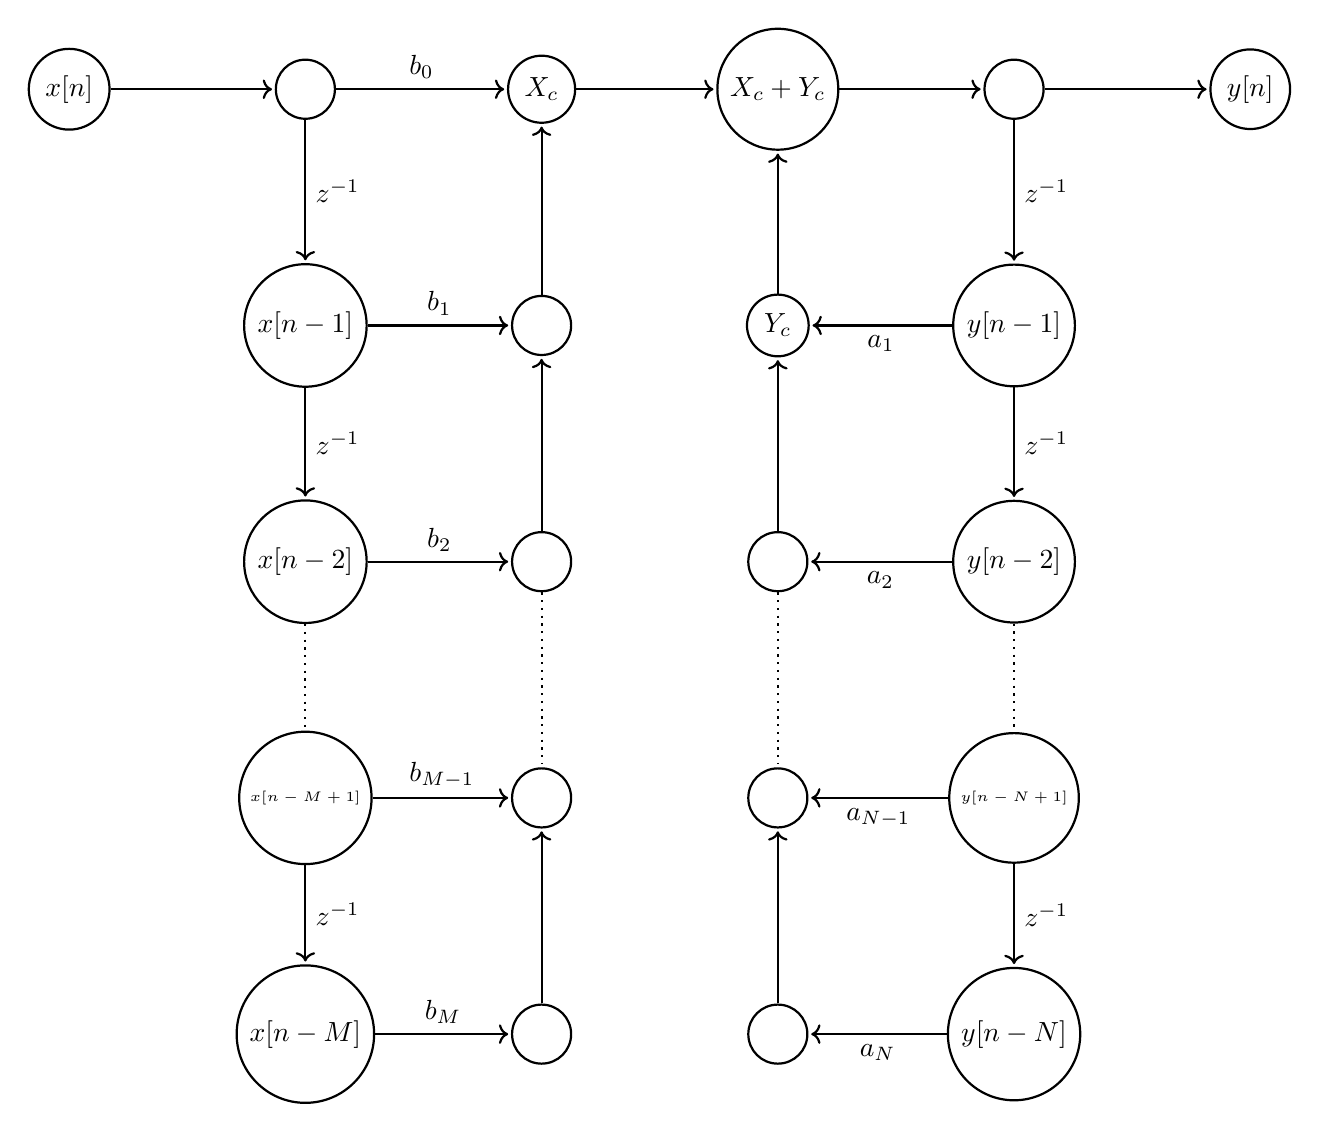
\begin{tikzpicture}[shorten >=1pt,node distance=3cm,on grid,auto]
    \tikzstyle{state}=[shape=circle,thick,draw,minimum size=0.75cm]

    \node[state] (A1) { $x[n]$};
    \node[state,right of=A1] (B1) {};
    \node[state,right of=B1] (C1) {$X_c$};
    \node[state, below of=B1] (B2) {$x[n-1]$};
    \node[state, below of=B2] (B3) {$x[n-2]$};
	\node[state, below of=B3] (B4) {\tiny $x[n-M+1]$};
    \node[state, below of=B4] (B5) {$x[n-M]$};
	\node[state, below of=C1] (C2) {};
	\node[state, below of=C2] (C3) {};
	\node[state, below of=C3] (C4) {};
	\node[state, below of=C4] (C5) {};
	
	\node[state, right of=C1] (D1) {$X_c + Y_c$};
	\node[state, right of=C2] (D2) {$Y_c$};
	\node[state, right of=C3] (D3) {};
	\node[state, right of=C4] (D4) {};
	\node[state, right of=C5] (D5) {};
	
	\node[state, right of=D1] (E1) {};
	\node[state, below of=E1] (E2) {$y[n-1]$};
	\node[state, below of=E2] (E3) {$y[n-2]$};
	\node[state, below of=E3] (E4) {\tiny $y[n-N+1]$};
	\node[state, below of=E4] (E5) {$y[n-N]$};
	
	\node[state, right of=E1] (F1){$y[n]$};


    \path[->,draw,thick]
    (A1) edge node {} (B1)
    (B1) edge node {$z^{-1}$} (B2)
    (B1) edge node {$b_0$} (C1)
	(B2) edge node {$z^{-1}$} (B3)
	(B4) edge node {$z^{-1}$} (B5)
	(B5) edge node {$b_M$} (C5)
	(B4) edge node {$b_{M-1}$} (C4)
	(B3) edge node {$b_2$} (C3)
	(B2) edge node {$b_1$} (C2)
	(C5) edge node {} (C4)
	(C3) edge node {} (C2)
	(C2) edge node {} (C1)
	(C1) edge node {} (D1)
	(D2) edge node {} (D1)
	(D5) edge node {} (D4)
	(D3) edge node {} (D2)
	(E1) edge node {$z^{-1}$} (E2) 
	(E2) edge node {$z^{-1}$} (E3) 
	(E4) edge node {$z^{-1}$} (E5)
	(E2) edge node {$a_1$} (D2) 
	(E3) edge node {$a_2$} (D3)
	(E4) edge node {$a_{N-1}$} (D4)
	(E5) edge node {$a_N$} (D5)
	(D1) edge node {} (E1) 
	(E1) edge node {} (F1)
    ;
	
	\draw[dotted, thick] (B3) -- (B4);
	\draw[dotted, thick] (C3) -- (C4);
	\draw[dotted, thick] (D3) -- (D4);
	\draw[dotted, thick] (E3) -- (E4);
	
  \end{tikzpicture}
  \caption{A Signal Flow Graph}
  \label{fig:sfg1}
\end{figure}


Evidently, there is a lot that's going on in the graph. First, I shall explain certain things about the graph. Each circle in the graph represents a \textbf{node}. All that a node does is hold a value. The directed lines connecting two nodes are called \textbf{edges}. Edges represent a \textit{transfer} of value from one node to the other. For example, the edge connecting $x[n]$ to the node on its right just copies the value $x[n]$ to the second node. Similarly, the second last node in the top row transfers or copies its value to the node $y[n]$. When an edge has a constant written on top of it, the effect of this is to multiply the value of the source node by the constant and transfer it to the destination node. For example, $y[n-N]$ is multiplied by $a_N$ and then transferred to the node to its left. When the multiplier is $z^{-1}$, the effect is to \textit{delay} the signal by one sample. Hence, the node containing $x[n]$ is multiplied by $z^{-1}$ giving us $x[n-1]$ in the node below. When a node has multiple input edges, the effect is to \textit{add} the values of all the source nodes. As shown, the node getting inputs from $X_c$ and $Y_c$ contains the value $X_c + Y_c$. \smallskip

It should now be clear as to what this graph is really doing. We first take the input $x[n]$. Delay it $M$ times and store the values $x[n] , x[n-1] \cdots x[n-M]$. We then multiply these by appropriate values $b_0, b_1 \cdots b_M$ and add them to store $X_c$. We follow the same procedure to calculate and store $Y_c$. Then, we add $X_c$ and $Y_c$ to give us $y[n] = X_c + Y_c$. To perform this operation for the next value of $x[n]$, we successively shift delay every sample by $1$ unit and repeat this procedure. \smallskip

The form of the graph shown in Figure \ref{fig:sfg1} is known as the \textbf{Direct Form I} graph. This graph easily translates into a hardware implementation of the system. We can perform the delay operations with the help of \textbf{registers} or \textbf{memory elements}. Multiplication can be carried out by constant multipliers and addition can be carried out by $2$-input adders.

Let us consider a numerical example. Consider the system function:

\[
    H(z) = \frac{8 - 3z^{-1}}{1-2z^{-1} + 5z^{-2}}
\]

To find the Direct Form I graph of this system, we first find the coefficients $b_l$ and $a_k$. Evidently, $b_0 = 8, b_1 = -3$ and $a_1 = 2, a_2 = -5$. The Direct Form I graph of this system is as follow.


\begin{figure}[!h]
  \centering
  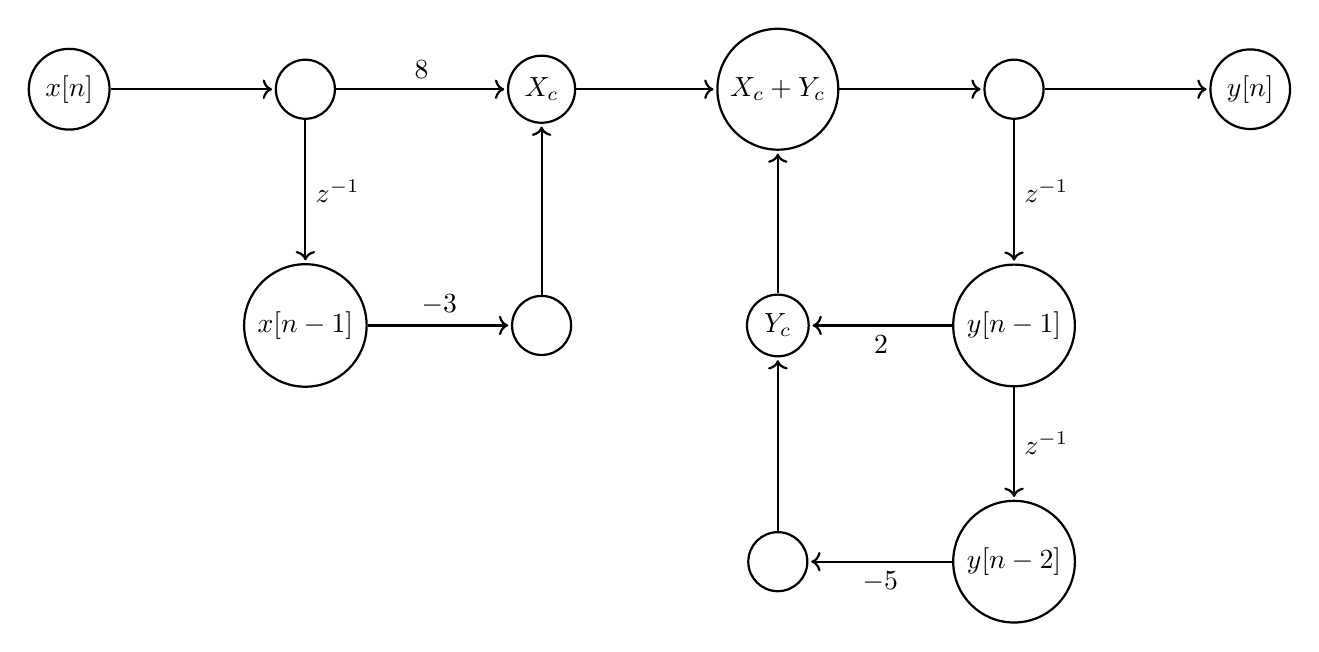
\begin{tikzpicture}[shorten >=1pt,node distance=3cm,on grid,auto]
    \tikzstyle{state}=[shape=circle,thick,draw,minimum size=0.75cm]

    \node[state] (A1) { $x[n]$};
    \node[state,right of=A1] (B1) {};
    \node[state, below of=B1] (B2) {$x[n-1]$};
    \node[state, right of=B1] (C1) {$X_c$};
    \node[state, below of=C1] (C2) {};
    \node[state, right of=C1] (D1) {$X_c + Y_c$};
    \node[state, below of=D1] (D2) {$Y_c$};
    \node[state, below of=D2] (D3) {};
    \node[state, right of=D1] (E1) {};
    \node[state, below of=E1] (E2) {$y[n-1]$};
    \node[state, below of=E2] (E3) {$y[n-2]$};
    \node[state, right of=E1] (F1) {$y[n]$};
    
    \path[->,draw,thick]
    (A1) edge node {} (B1)
    (B1) edge node {$z^{-1}$} (B2)
    (B2) edge node {$-3$} (C2)
    (B1) edge node {$8$} (C1)
    (C2) edge node {} (C1)
    (C1) edge node {} (D1)
    (D1) edge node {} (E1)
    (E1) edge node {$z^{-1}$} (E2)
    (E2) edge node {$z^{-1}$} (E3)
    (E2) edge node {$2$} (D2)
    (E3) edge node {$-5$} (D3)
    (D3) edge node {} (D2)
    (D2) edge node {} (D1)
    (E1) edge node {} (F1)
   ;
	
  \end{tikzpicture}
  \caption{Direct Form I Graph of the given system} 
  \label{fig:sfg2}
\end{figure}

Note: There are two redundant nodes present in the above graph - namely the one between $x[n-1]$ and $X_c$ and the one between $y[n-2]$ and $Y_c$. We can remove these nodes. A more concise and efficient graph is shown below.

\begin{figure}[!h]
  \centering
  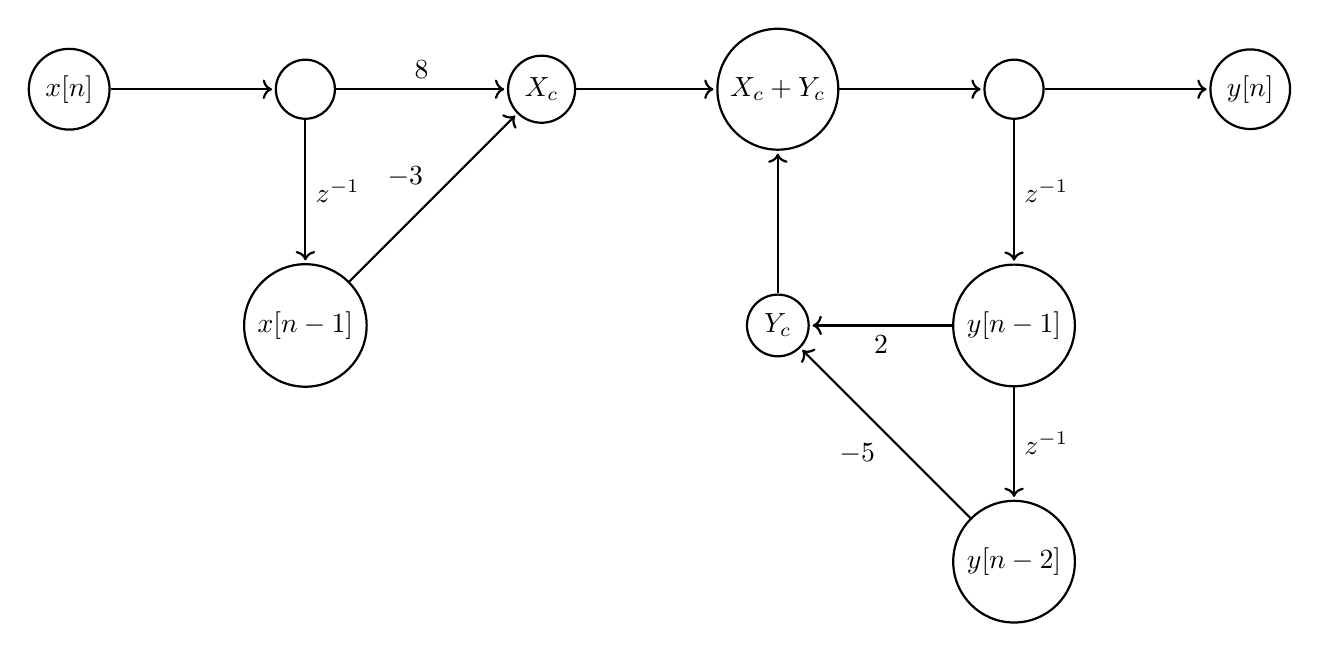
\begin{tikzpicture}[shorten >=1pt,node distance=3cm,on grid,auto]
    \tikzstyle{state}=[shape=circle,thick,draw,minimum size=0.75cm]

    \node[state] (A1) { $x[n]$};
    \node[state,right of=A1] (B1) {};
    \node[state, below of=B1] (B2) {$x[n-1]$};
    \node[state, right of=B1] (C1) {$X_c$};
    \node[state, right of=C1] (D1) {$X_c + Y_c$};
    \node[state, below of=D1] (D2) {$Y_c$};
    \node[state, right of=D1] (E1) {};
    \node[state, below of=E1] (E2) {$y[n-1]$};
    \node[state, below of=E2] (E3) {$y[n-2]$};
    \node[state, right of=E1] (F1) {$y[n]$};
    
    \path[->,draw,thick]
    (A1) edge node {} (B1)
    (B1) edge node {$z^{-1}$} (B2)
    (B2) edge node {$-3$} (C1)
    (B1) edge node {$8$} (C1)
    (C1) edge node {} (D1)
    (D1) edge node {} (E1)
    (E1) edge node {$z^{-1}$} (E2)
    (E2) edge node {$z^{-1}$} (E3)
    (E2) edge node {$2$} (D2)
    (E3) edge node {$-5$} (D2)
    (D2) edge node {} (D1)
    (E1) edge node {} (F1)
   ;
	
  \end{tikzpicture}
  \caption{Simplified Direct Form I Graph of the given system} 
  \label{fig:sfg3}
\end{figure}

It is clear to see why such a graph is called a Signal Flow Graph. Such a graph simply represents the flow of signals from the source nodes through the intermediate nodes and finally to the output nodes along with the operations performed in the middle. I would encourage you to try devising a software implementation of this system, i.e, a pseudo-code for arriving at the output from the input.

\subsection{The Direct Form II Graph}

We can design a different form of the general rational causal LSI system by treating its system function in a different way. Consider the general system function, $H(z)$. We can break $H(z)$ into two parts - the one originating from the poles and the one originating from the zeros - and equivalently write it as:

\[
    H(z) = \left( \ddfrac{1}{1 - \sum_{k=1}^{N} a_k z^{-k}} \right) \cdot \left( \sum_{l=0}^{M} b_l z^{-l} \right) = H_{pole}(z) \cdot H_{zero}(z)
\]

This gives us another way of implementing the system, as shown in Figure \ref{fig:sfg4}.

\begin{figure}[!h]
  \centering
  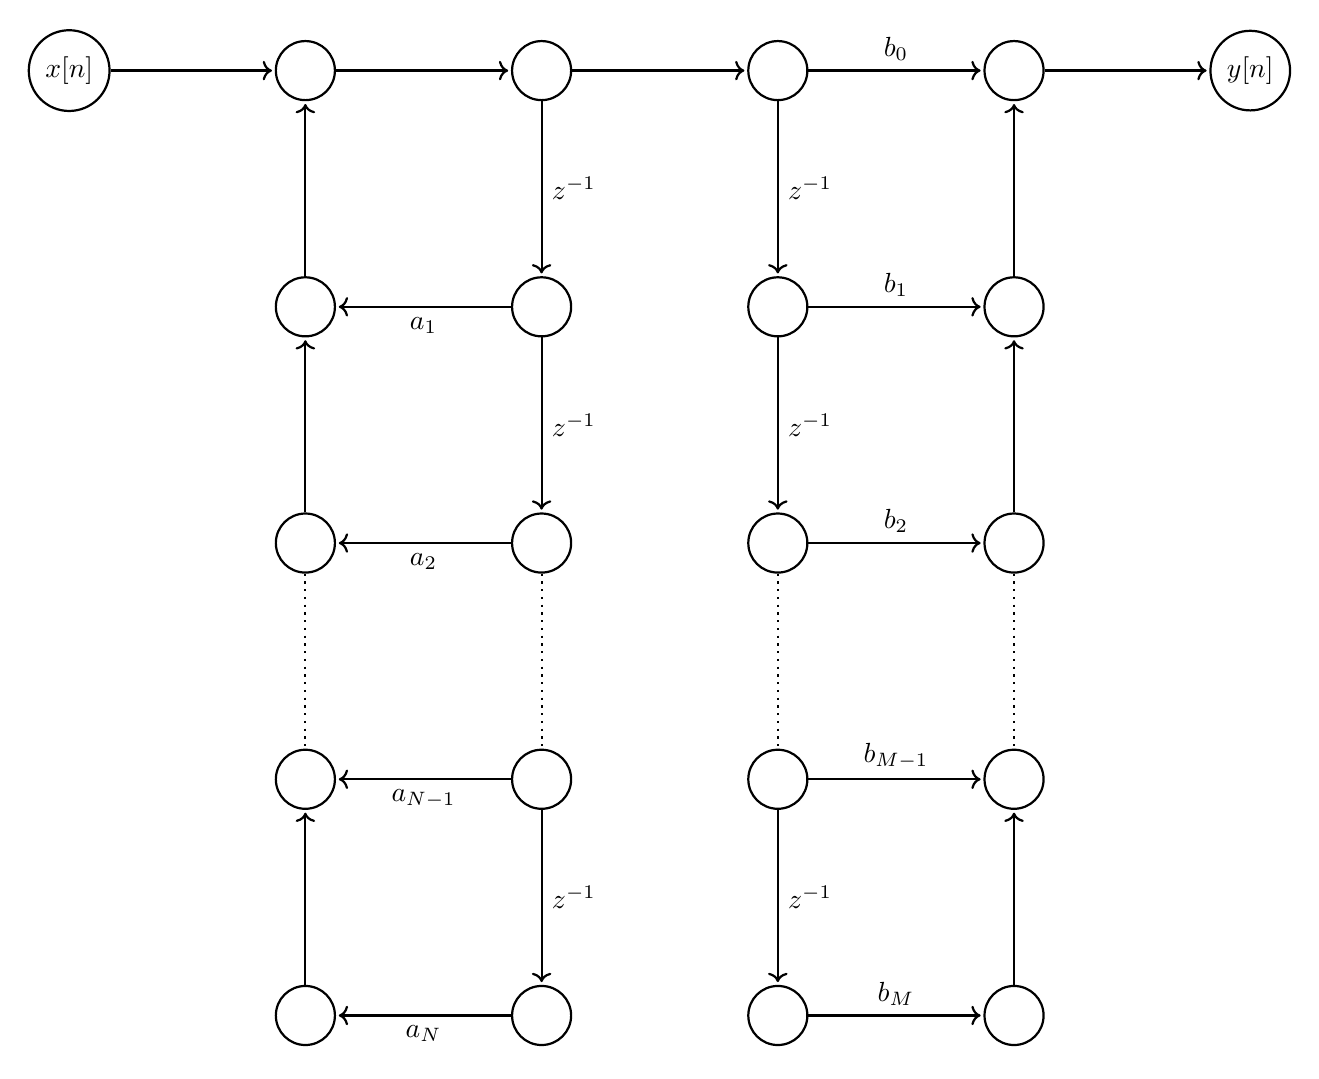
\begin{tikzpicture}[shorten >=1pt,node distance=3cm,on grid,auto]
    \tikzstyle{state}=[shape=circle,thick,draw,minimum size=0.75cm]

    \node[state] (A1) { $x[n]$};
    \node[state,right of=A1] (B1) {};
    \node[state,right of=B1] (C1) {};
    \node[state, below of=B1] (B2) {};
    \node[state, below of=B2] (B3) {};
	\node[state, below of=B3] (B4) {};
    \node[state, below of=B4] (B5) {};
	\node[state, below of=C1] (C2) {};
	\node[state, below of=C2] (C3) {};
	\node[state, below of=C3] (C4) {};
	\node[state, below of=C4] (C5) {};
	
	\node[state, right of=C1] (D1) {};
	\node[state, right of=C2] (D2) {};
	\node[state, right of=C3] (D3) {};
	\node[state, right of=C4] (D4) {};
	\node[state, right of=C5] (D5) {};
	
	\node[state, right of=D1] (E1) {};
	\node[state, below of=E1] (E2) {};
	\node[state, below of=E2] (E3) {};
	\node[state, below of=E3] (E4) {};
	\node[state, below of=E4] (E5) {};
	
	\node[state, right of=E1] (F1){$y[n]$};


    \path[->,draw,thick]
    (A1) edge node {} (B1)
    (B2) edge node {} (B1)
    (B1) edge node {} (C1)
	(B3) edge node {} (B2)
	(B5) edge node {} (B4)
	(C5) edge node {$a_N$} (B5)
	(C4) edge node {$a_{N-1}$} (B4)
	(C3) edge node {$a_2$} (B3)
	(C2) edge node {$a_1$} (B2)
	(C4) edge node {$z^{-1}$} (C5)
	(C2) edge node {$z^{-1}$} (C3)
	(C1) edge node {$z^{-1}$} (C2)
	(C1) edge node {} (D1)
	(D1) edge node {$z^{-1}$} (D2)
	(D4) edge node {$z^{-1}$} (D5)
	(D2) edge node {$z^{-1}$} (D3)
	(E2) edge node {} (E1) 
	(E3) edge node {} (E2) 
	(E5) edge node {} (E4)
	(D2) edge node {$b_1$} (E2) 
	(D3) edge node {$b_2$} (E3)
	(D4) edge node {$b_{M-1}$} (E4)
	(D5) edge node {$b_M$} (E5)
	(D1) edge node {$b_0$} (E1) 
	(E1) edge node {} (F1)
    ;
	
	\draw[dotted, thick] (B3) -- (B4);
	\draw[dotted, thick] (C3) -- (C4);
	\draw[dotted, thick] (D3) -- (D4);
	\draw[dotted, thick] (E3) -- (E4);
	
  \end{tikzpicture}
  \caption{An Alternative Signal Flow Graph}
  \label{fig:sfg4}
\end{figure}

We can consider the entire system to be a \textit{cascade} of the two systems $H_{\text{pole}}(z)$ and $H_{\text{zero}}(z)$ (known as all-pole and all-zero systems respectively). Their impulse response will be a convolution of the impulse responses of the pole and zero parts. $h_{eq}[n] = h_{\text{pole}}[n] * h_{\text{zero}}[n]$. By associativity of convolution, we have that $x*(h_{\text{pole}} * h_{\text{zero}})$ = $(x*h_{\text{pole}}) * h_{\text{zero}}$. Hence, the system acts like a cascade. The output produced from the pole system is fed as an input to the zero system. This is the idea we have used in Figure \ref{fig:sfg4}. However, note that the $3^{\text{rd}}$ and $4^{\text{th}}$ columns are identical, hence redundant. We can further simplify the structure by merging these two columns. 

\begin{figure}[!h]
  \centering
  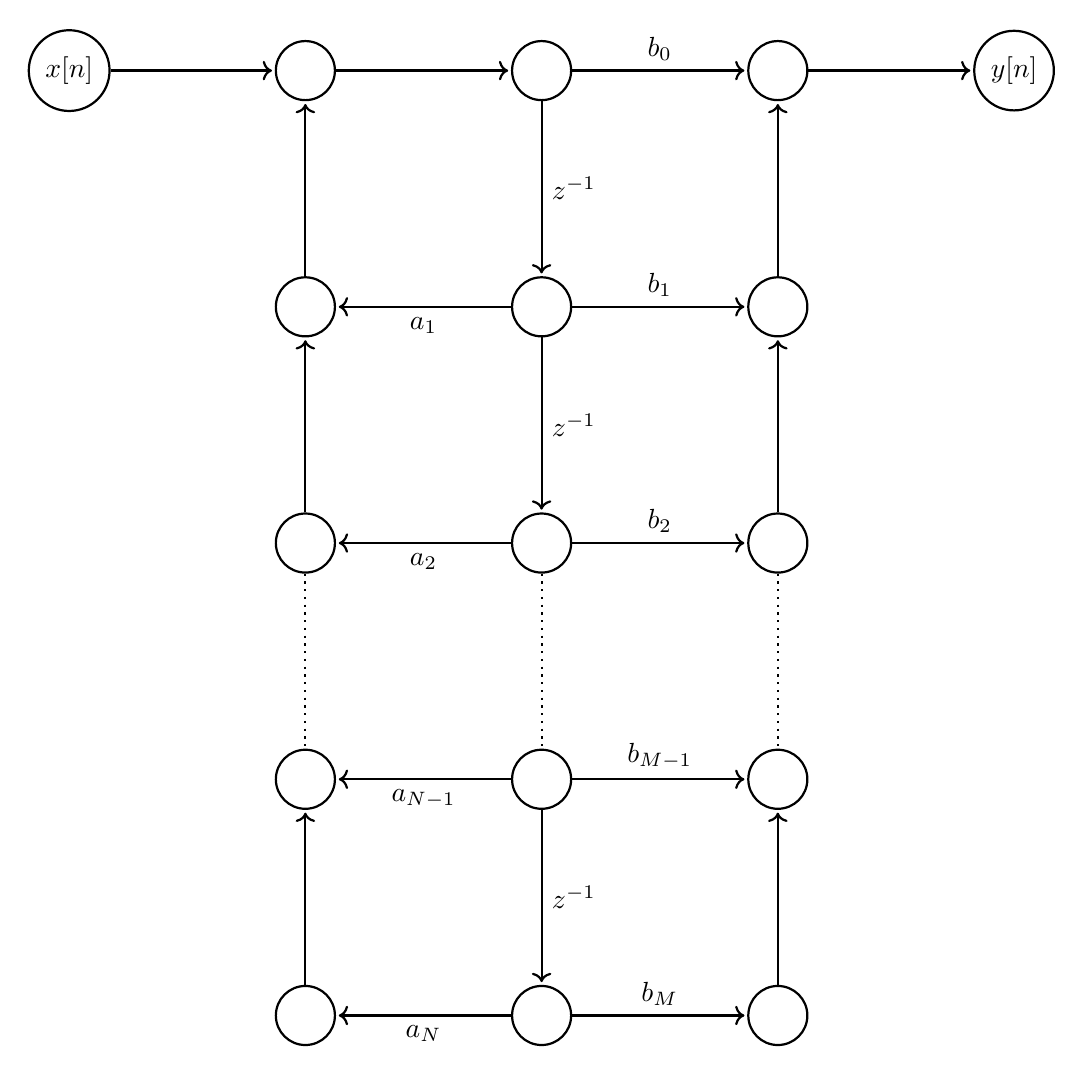
\begin{tikzpicture}[shorten >=1pt,node distance=3cm,on grid,auto]
    \tikzstyle{state}=[shape=circle,thick,draw,minimum size=0.75cm]

    \node[state] (A1) { $x[n]$};
    \node[state,right of=A1] (B1) {};
    \node[state,right of=B1] (C1) {};
    \node[state, below of=B1] (B2) {};
    \node[state, below of=B2] (B3) {};
	\node[state, below of=B3] (B4) {};
    \node[state, below of=B4] (B5) {};
	\node[state, below of=C1] (C2) {};
	\node[state, below of=C2] (C3) {};
	\node[state, below of=C3] (C4) {};
	\node[state, below of=C4] (C5) {};
	
	\node[state, right of=C1] (D1) {};
	\node[state, right of=C2] (D2) {};
	\node[state, right of=C3] (D3) {};
	\node[state, right of=C4] (D4) {};
	\node[state, right of=C5] (D5) {};

	\node[state, right of=D1] (E1){$y[n]$};


    \path[->,draw,thick]
    (A1) edge node {} (B1)
    (B2) edge node {} (B1)
    (B1) edge node {} (C1)
	(B3) edge node {} (B2)
	(B5) edge node {} (B4)
	(C5) edge node {$a_N$} (B5)
	(C4) edge node {$a_{N-1}$} (B4)
	(C3) edge node {$a_2$} (B3)
	(C2) edge node {$a_1$} (B2)
	(C4) edge node {$z^{-1}$} (C5)
	(C2) edge node {$z^{-1}$} (C3)
	(C1) edge node {$z^{-1}$} (C2)
	(D2) edge node {} (D1) 
	(D3) edge node {} (D2) 
	(D5) edge node {} (D4)
	(C2) edge node {$b_1$} (D2) 
	(C3) edge node {$b_2$} (D3)
	(C4) edge node {$b_{M-1}$} (D4)
	(C5) edge node {$b_M$} (D5)
	(C1) edge node {$b_0$} (D1) 
	(D1) edge node {} (E1)
    ;
	
	\draw[dotted, thick] (B3) -- (B4);
	\draw[dotted, thick] (C3) -- (C4);
	\draw[dotted, thick] (D3) -- (D4);
	
  \end{tikzpicture}
  \caption{The Direct Form II Graph}
  \label{fig:sfg5}
\end{figure}

This is known as the \textbf{Direct Form II Graph}. Note, the middle branch extends for $\max(N,M)$ nodes. Figure \ref{fig:sfg7} shows the Direct Form II Graph of the system we mentioned above. Note again, that there are redundant nodes. Eliminating them, we arrive at Figure \ref{fig:sfg8}, the simplified Direct Form II Graph of the system. We see that both the Direct Form I and II graphs utilise the same number of adders and multipliers, but the Direct Form II is much more economical in delays. The Direct Form II uses $\max(N,M)$ delays while the Direct Form I uses $N+M$ delays.

\begin{figure}[!h]
  \centering
  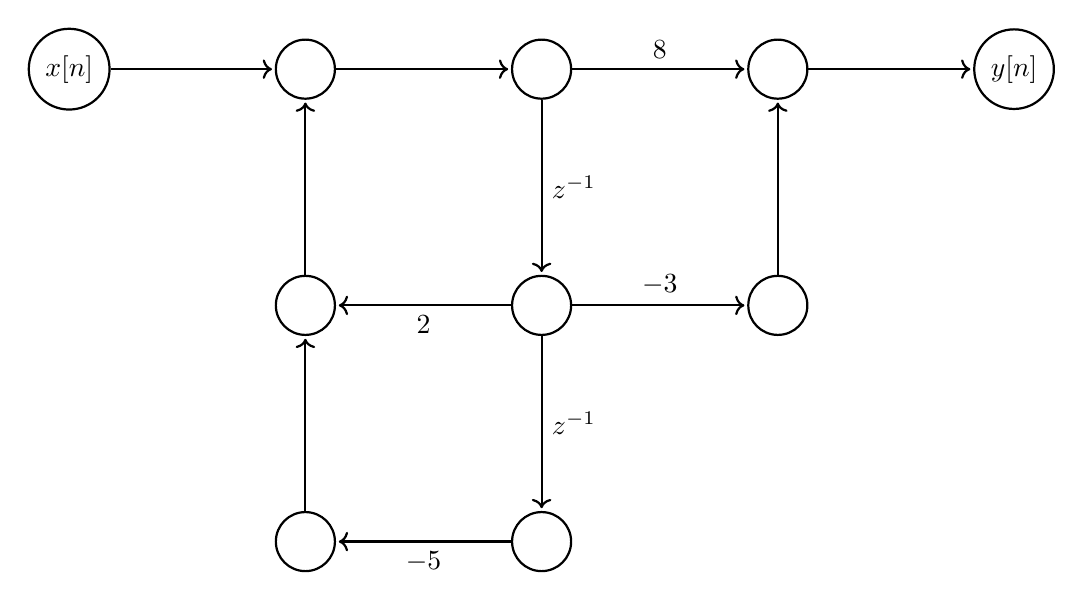
\begin{tikzpicture}[shorten >=1pt,node distance=3cm,on grid,auto]
    \tikzstyle{state}=[shape=circle,thick,draw,minimum size=0.75cm]

    \node[state] (A1) { $x[n]$};
    \node[state,right of=A1] (B1) {};
    \node[state, below of=B1] (B2) {};
    \node[state, below of=B2] (B3) {};
    \node[state, right of=B1] (C1) {};
    \node[state, below of=C1] (C2) {};
    \node[state, below of=C2] (C3){};
    \node[state, right of=C1] (D1) {};
    \node[state, below of=D1] (D2) {};
    \node[state, right of=D1] (E1) {$y[n]$};
    
    \path[->,draw,thick]
    (A1) edge node {} (B1)
    (B2) edge node {} (B1)
    (C2) edge node {$2$} (B2)
    (B1) edge node {} (C1)
    (C1) edge node {$z^{-1}$} (C2)
    (C2) edge node {$z^{-1}$} (C3)
    (C3) edge node {$-5$} (B3)
    (C1) edge node {$8$} (D1)
    (C2) edge node {$-3$} (D2)
    (D2) edge node {} (D1)
    (D1) edge node {} (E1)
    (B3) edge node {} (B2)
   ;
	
  \end{tikzpicture}
  \caption{Direct Form II Graph of the given system} 
  \label{fig:sfg7}
\end{figure}

\begin{figure}[!h]
  \centering
  \begin{tikzpicture}[shorten >=1pt,node distance=3cm,on grid,auto]
    \tikzstyle{state}=[shape=circle,thick,draw,minimum size=0.75cm]

    \node[state] (A1) { $x[n]$};
    \node[state,right of=A1] (B1) {};
    \node[state, below of=B1] (B2) {};
    \node[state, right of=B1] (C1) {};
    \node[state, below of=C1] (C2) {};
    \node[state, below of=C2] (C3){};
    \node[state, right of=C1] (D1) {};
    \node[state, right of=D1] (E1) {$y[n]$};
    
    \path[->,draw,thick]
    (A1) edge node {} (B1)
    (B2) edge node {} (B1)
    (C2) edge node {$2$} (B2)
    (B1) edge node {} (C1)
    (C1) edge node {$z^{-1}$} (C2)
    (C2) edge node {$z^{-1}$} (C3)
    (C3) edge node {$-5$} (B2)
    (C1) edge node {$8$} (D1)
    (C2) edge node {$-3$} (D1)
    (D1) edge node {} (E1)
   ;
	
  \end{tikzpicture}
  \caption{Simplified Direct Form II Graph of the given system} 
  \label{fig:sfg8}
\end{figure}

\clearpage

\subsection{Cascade and Parallel Decomposition}

In the Direct Form II Graph, we expressed $H(z)$ as a cascade of two systems $H_{\text{pole}}(z)$ and $H_{\text{zero}}(z)$. Expanding on this idea, we could've as well expressed $H(z)$ as a cascade of many such systems, or :

\[
    H(z) = H_1(z) \cdot H_2(z) \ldots H_Q(z) 
\]

where each $H_i(z)$ includes some of the poles and/or some of the zeros. Such a decomposition of $H(z)$ is known as a \textbf{Cascade Decomposition}. Evidently, there is an enormous number of ways in which we can perform this decomposition. Different decompositions or factorisations lead to different realisations of the system. The basic rule is that if we have a pair of complex conjugate poles/zeroes then we prefer keeping them together. A general cascade form of a system is shown below:

\begin{figure}[!h]
  \centering
  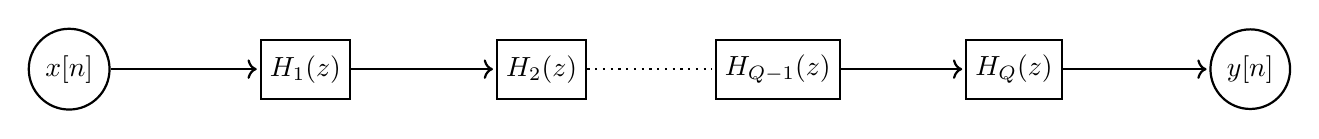
\begin{tikzpicture}[shorten >=1pt,node distance=3cm,on grid,auto]
    \tikzstyle{state}=[shape=circle,thick,draw,minimum size=0.75cm]
    \tikzstyle{process}=[shape=rectangle,thick,draw,minimum size=0.75cm]

    \node[state] (A) { $x[n]$};
    \node[process,right of=A] (B) {$H_1(z)$};
    \node[process,right of=B] (C) {$H_2(z)$};
    \node[process,right of=C] (D) {$H_{Q-1}(z)$};
    \node[process,right of=D] (E) {$H_Q(z)$};
    \node[state,right of=E] (F) {$y[n]$};
    
    \path[->,draw,thick]
    (A) edge node {} (B)
    (B) edge node {} (C)
    (D) edge node {} (E) 
    (E) edge node {} (F)
   ;
   \draw[dotted, thick] (C) -- (D);
	
  \end{tikzpicture}
  \caption{A Cascade Form} 
  \label{fig:sfg9}
\end{figure}

Another method of decomposing $H(z)$ is when we express it as a \textit{sum} of terms. These terms are of two forms:

\begin{enumerate}
    \item 
    \[
        \frac{N_1(z^{-1})}{(1-\alpha z^{-1})^P}
    \]
    where $\alpha$ is a real pole of the system having multiplicity $P$ and $N_1(z^{-1})$ is a polynomial in $z^{-1}$ having degree less than $P$.
    \item 
    \[
        \frac{N_2(z^{-1})}{(1-\beta z^{-1})^P \cdot (1-\overline{\beta} z^{-1})^P}
    \]
    where $\beta, \overline{\beta}$ are complex conjugate poles of the system having multiplicity $P$ and $N_2(z^{-1})$ is a polynomial in $z^{-1}$ having degree less than $2P$.
\end{enumerate}

After determining these terms, we can write $H(z)$ as a sum of these terms. Consequently, the system can be implemented by putting all these sub-systems in parallel (Hint: use linearity of the Z Transform). Such a decomposition is known as a \textbf{Parallel Decomposition}. The parallel form of the system is shown in Figure \ref{fig:sfg10}. Note: while the decomposition of $H(z)$ into parallel components is unique, each term can further be expressed as a cascade in many forms. Hence, the form of the signal flow graph shown in Figure \ref{fig:sfg10} is sometimes also known as a \textbf{Parallel-Cascade Form}. Thus, we have encountered the following forms of signal flow graphs:

\begin{enumerate}
    \item Direct Form I Graph
    \item Direct Form II Graph
    \item Cascade Form 
    \item Parallel Form (or Parallel-Cascade Form)
\end{enumerate}

\begin{figure}[!h]
  \centering
  \begin{tikzpicture}[shorten >=1pt,node distance=3cm,on grid,auto]
    \tikzstyle{state}=[shape=circle,thick,draw,minimum size=0.75cm]
    \tikzstyle{process}=[shape=rectangle,thick,draw,minimum size=0.75cm]

    \node[state] (A) { $x[n]$};
    \node[state, right of=A] (B3) {};
    \node[state, above of=B3] (B2){};
    \node[state, above of=B2] (B1){};
    \node[state, below of=B3] (B4){};
    \node[state, below of=B4] (B5){};
    \node[process, right of=B1] (C1) {$H_1(z)$};
    \node[process, right of=B2] (C2) {$H_2(z)$};
    \node[process, right of=B3] (C3) {$H_i(z)$};
    \node[process, right of=B4] (C4) {$H_{Q-1}(z)$};
    \node[process, right of=B5] (C5) {$H_Q(z)$};
    \node[state, right of=C1] (D1) {};
    \node[state, right of=C2] (D2) {};
    \node[state, right of=C4] (D4) {};
    \node[state, right of=C5] (D5) {};
    \node[state, below of=D2] (D3) {};
    \node[state, right of=D3] (E) {$y[n]$};
    
    \path[->,draw,thick]
    (A) edge node {} (B3)
    (B2) edge node {} (B1)
    (B4) edge node {} (B5)
    (B1) edge node {} (C1)
    (B2) edge node {} (C2)
    (B4) edge node {} (C4)
    (B5) edge node {} (C5)
    (C1) edge node {} (D1)
    (C2) edge node {} (D2)
    (C4) edge node {} (D4)
    (C5) edge node {} (D5)
    (D1) edge node {} (D2)
    (D5) edge node {} (D4)
    (D3) edge node {} (E)
    (B3) edge node {} (C3)
    (C3) edge node {} (D3)
   ;
   \draw[->, dotted, thick] (B3) -- (B4);
   \draw[dotted, thick] (C2) -- (C3);
   \draw[dotted, thick] (C4) -- (C3);
   \draw[->, dotted, thick] (D4) -- (D3);
   \draw[->, dotted, thick] (B3) -- (B2);
   \draw[->, dotted, thick] (D2) -- (D3);
	
  \end{tikzpicture}
  \caption{A Parallel Form} 
  \label{fig:sfg10}
\end{figure}

\clearpage

\subsection{Difference Equations}

\begin{defn}
Difference equations are equations involving are the discrete analogue of differential equations, involving differences between successive values of a sequence.
\end{defn}

In particular, we wish to focus on the solutions of a particular class of difference equations, known as \textbf{Linear Constant Coefficient Difference Equations} or LCCDE's. A general LCCDE can be represented as :

\[
    y[n] = \sum_{k=1}^{N} a_k y[n-k] + \sum_{l=0}^{M} b_l x[n-l]
\]

Suppose we wish to find the solution $y[n]$, for a given input $x[n]$, having a rational Z transform $X(z)$. If the LCCDE holds over all $n$, we could quite easily take Z transform on both sides of the difference equation, giving us:

\[
    Y(z) = H(z) \cdot X(z) \quad \text{and} \quad y[n] = \mathcal{Z}^{-1} \{ Y(z) \}
\]

Here, $H(z)$ is the system function we discussed above. As both $H(z)$ and $X(z)$ are rational, $Y(z)$ is also rational, hence its inverse Z transform is easily obtainable. However, we can only use this method when the LCCDE holds for all $n$. We wish to analyse and solve this difference equation even when it holds for a restricted interval of $n$.

Consider, for example the LCCDE:

\[
    y[n] = \frac{1}{2}y[n-1] + y[n-2] + 3x[n] \quad \text{for} \quad n \geq 0
\]

The input provided is $x[n] = \alpha^n \quad \text{for} \quad n \geq 0$. In order to solve this LCCDE, we either need $y[-1] \text{and} y[-2]$, or we need the value of $y[n]$ at any two points in the interval of interest - namely, $n \geq 0$.

Consider for a moment that we allow the LCCDE to hold for all $n$. Then, we can write:

\[
    H(z) = \frac{3}{1 - \frac{1}{2}z^{-1} + z^{-2}}
\]

and, we could extend $x[n]$ to be $x[n] = \alpha^n \cdot u[n]$, which takes the same value as the original sequence in our interval of interest $n \geq 0$. The purpose of extending $x[n]$ this way was to obtain a sequence which has a \textit{rational} Z transform while retaining the value of the sequence in the interval of interest. We now consider inputs $x[n]$ which can be extended in this way. Let $x[n]$ be extended to the form $\sum Q(n) \cdot \alpha^n$ - namely, sum of exponentials multiplied by polynomials in $n$. After having done this, we can solve the equation in the $z$-domain, by writing: $Y(z) = H(z) \cdot X(z)$. We can find the poles of $Y(z)$ and subsequently, solve for $y[n]$. The solution of the difference equation essentially depends on the following:

\begin{enumerate}
    \item Poles of the system ($H(z)$) and their multiplicity. 
    \item Exponential factors in $x[n]$ and the degree of the polynomial associated with each such factor. (The coefficients of the polynomial itself are irrelevant).
\end{enumerate} \medskip

\textbf{Example.} Consider that we wish to solve the equation $y[n] = \frac{1}{3} y[n-1] + x[n]$ for $n \geq 0$, for the input $x[n] = (\frac{1}{2})^n \quad \text{for} n \geq 0$. The corresponding system function is given by: 

\[
    H(z) = \frac{1}{1 - \frac{1}{3}z^{-1}} 
\]

The poles can be classified as follows:

\begin{enumerate}
    \item System poles $\rightarrow$ at $\frac{1}{3}$
    \item Input poles $\rightarrow$ at $\frac{1}{2}$
\end{enumerate}

These poles are distinct and do not have a non-null intersection. Hence, the overall response will have two terms - one arising from the system pole and one from the input pole. 

In general, the response will have 3 components:

\begin{enumerate}
    \item \textbf{Forced Response:} contributed by the input poles alone
    \item \textbf{Natural Response:} contributed by the system poles alone
    \item \textbf{Resonant Response:} contributed by the common poles - or poles which are a part of both the system and the input. 
\end{enumerate}

To illustrate these three components and how to solve such equations, we take up an example. 

\textbf{Example.} Consider the system described by the following equations.

\[
    H(z) = \frac{N(z^{-1})}{(1 - \frac{1}{3}z^{-1})^2 \cdot (1 - \frac{1}{4}z^{-1})}  = \frac{N(z^{-1})}{1 - (\alpha_1z^{-1} + \alpha_2z^{-2} + \alpha_3z^{-3})}
\]
\[
    x[n] = \left(\frac{1}{3}\right)^n + \left(\frac{1}{5}\right)^n \quad \text{for} \quad n \geq 0
\]

We wish to solve the corresponding LCCDE for $n \geq 0$. Note: $H(z)$ is the system function we obtain by letting the LCCDE hold for all $n$. The corresponding LCCDE can be written as:

\[
    y[n] = \alpha_1y[n-1] + \alpha_2y[n-2] + \alpha_3y[n-3] + \sum_{l=0}^{M} b_l x[n-l]
\]

The value of $M$ and coefficients $b_l$ depend on the numerator $N(z^{-1})$. First, let us group the poles: 

\begin{enumerate}
    \item System poles : $(\frac{1}{3} , \frac{1}{3})$ , $\frac{1}{4}$
    \item Input poles : $\frac{1}{3} , \frac{1}{5}$
\end{enumerate}

The system and input poles have a non-null intersection: $\frac{1}{3}$. Now, the final solution will consist of the following components:

\begin{enumerate}
    \item Forced response from the pole $(\frac{1}{5})$ of the form $A_1 (\frac{1}{5})^n$ for $n \geq 0$
    \item Natural response from the pole $(\frac{1}{4})$ of the form $A_2 (\frac{1}{4})^n$ for $n \geq 0$
    \item Resonant response from the pole $(\frac{1}{3})$ of the form $(A_3n^2 + A_4n + A_5) \cdot (\frac{1}{3})^n$ for $n \geq 0$
\end{enumerate}

Note, the polynomial corresponding to the resonant response is of degree two because the corresponding pole $\frac{1}{3}$ has multiplicity three. Hence, the final solution of $y[n]$ is 
\[
    y[n] = A_1 \left( \frac{1}{5}\right)^n + A_2 \left( \frac{1}{4} \right)^n + (A_3n^2 + A_4n + A_5) \cdot \left( \frac{1}{3} \right)^n \quad \text{for} \quad n \geq 0
\]

All that remains is finding the constants $A_1, \ldots ,A_5$. 

We can solve the equation via the recurrence relation directly if we know the values of $y[-1], y[-2]$ and $y[-3]$ or any three \textbf{independent} values of $y[n]$ in the region of applicability. Note: the term `independent' is important as redundant information will not help us.  \smallskip

At this point, it may strike your mind that we are able to solve for $y[n]$ by having only three conditions with us. But our expression for $y[n]$ as the sum of exponentials gives the impression that we need \textbf{five} equations to determine the five constants and hence $y[n]$ itself. The explanation is that we need only three conditions to solve completely for $y[n]$ but doing so will allow us to describe the solution only through a recursive definition of $y[n]$. However, determining the five constants $A_1, \ldots ,A_5$ allows us to obtain a \textit{closed-form} expression for $y[n]$.  \smallskip

Let us now try to obtain the constants $A_1, \ldots ,A_5$. We need five independent conditions to solve for these constants. Three of these can be found using outputs $y[0], y[1]$ and $y[2]$. Note, we can't use $y[3]$ and $y[4]$ as separate conditions as they are not independent of the initial three conditions. The last two conditions by noting the following. 

\begin{enumerate}
    \item the forced response must satisfy the difference equation by itself.
    \item the resonant response must satisfy the difference equation by itself.
\end{enumerate}

That is, the resonant and forced components of the response and their corresponding input exponentials must itself satisfy the difference equation. We can obtain the final two conditions this way. Consider that $X(z) = \frac{Y(z)}{H(z)}$. A convenient way to arrive at the final conditions is to take the inverse transform. We consider the term $(H(z))^{-1}$ to act as an \textit{operator} on $y[n]$. 

\[
    \text{Define} \quad \hat{H} = \frac{1}{H(z)} = \left[ \left( 1 - \frac{1}{4}z^{-1}  \right) \cdot \left( 1 - \frac{1}{3}z^{-1} \right)^2 \right] \quad \text{to be an operator}.
\]

$\hat{H}$ acts on the Z transform of $y[n]$, $Y(z)$ and then converts it to the discrete-time domain. By what we said earlier, we must have $\hat{H} y = x$ for the forced and resonant responses. The operator $\hat{H}$ is actually a cascade of three operations:

\begin{enumerate}
    \item $y[n] \mapsto y[n] - \frac{1}{4} y[n-1]$
    \item $y[n] \mapsto y[n] - \frac{1}{3}y[n-1] \quad$ applied twice.
\end{enumerate}

First, let us consider the forced response $A_1 (\frac{1}{5})^n$ and the corresponding input $(\frac{1}{5})^n$. When we apply the first operation on this, we get:

\[
    y[n] - \frac{1}{4}y[n-1] = A_1 \left( \frac{1}{5}\right)^n - A_1 \frac{1}{4} \left( \frac{1}{5}\right)^n = A_1 \left( \frac{1}{5}\right)^n \left[ 1 - \frac{1}{4}z^{-1} \right] \quad \text{at} \quad z = \frac{1}{5}
\]
So, the sequence we obtain our cascading all three operations must be equal to the original input. Hence, 

\[
    A_1 \left(\frac{1}{5}\right)^n \left[ \left( 1 - \frac{1}{4}z^{-1}  \right) \cdot \left( 1 - \frac{1}{3}z^{-1} \right)^2 \right] \quad \text{at} \quad z= \frac{1}{5}
\]
\[
    \therefore A_1 \cdot \left( 1 - \frac{5}{4}\right) \cdot \left( 1 - \frac{5}{3}\right)^2 \cdot \left(\frac{1}{5} \right)^n = \left( \frac{1}{5}\right)^n
\]

From the above equation, we can find $A_1$. In general, the equation would be of the form :

\[
    A_1 \cdot \left( 1 - \frac{5}{4}\right) \cdot \left( 1 - \frac{5}{3}\right)^2 \cdot \left(\frac{1}{5} \right)^n =  \left[ \sum_{l=0}^{M} b_l \left(\frac{1}{5} \right)^{-l}\right] \cdot \left( \frac{1}{5}\right)^n 
\]

Thus, we have found out $A_1$. I will leave the calculations for the resonant response part to you. You would interestingly find that only the highest degree term in $n (A_3)$ will survive. Hence, we have now found out $A_3$ and $A_1$. We can find $A_2, A_4$ and $A_5$ from the three output conditions and obtain the complete closed form of the response $y[n]$. \smallskip

Hence, we have found a method of solving a general LCCDE. We can also divide our intervals as $0$ to $n_0$, $n_0$ to $n_1$, $n_1$ to $n_2$ and so on. The last few outputs of a certain range will act as the initial conditions of the next range. Hence, we have practically solved the problem of piece-wise LCCDE's, i.e, systems which satisfy different LCCDE's in different intervals.
Now, we move on to the synthesis of discrete-time systems.

\section{Synthesis of Discrete-Time Systems}

\subsection{The Ideal Filter}

In this section, we will be designing discrete-time filters. A filter is essentially a system which performs mathematical operations on a signal to enhance or suppress certain aspects of that signal. For example, a low pass filter enhances the low frequencies of the signal while it suppresses the high frequencies. The frequency response of the ideal low pass filter is shown in Figure \ref{fig:low_pass_ideal}

\begin{figure}[h!]
\centering
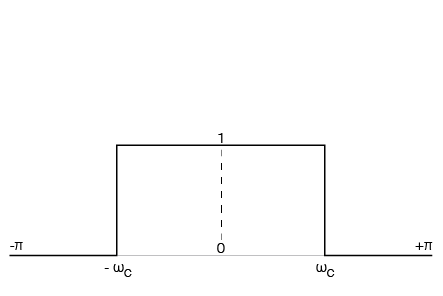
\includegraphics[width = 75mm, scale = 3]{low_pass_ideal.png}
\caption{Frequency Response of an Ideal Low-Pass Filter}
\label{fig:low_pass_ideal}
\end{figure}	 

Clearly, it retains frequencies between $-\omega_c$ and $\omega_c$ and throws out the others. The impulse response for this filter is given by:

\[
	h[n] = 
	\begin{dcases}
    \frac{\sin(\omega_c n)}{\pi n} & n \neq 0 \\
    \frac{\omega_c}{\pi} & n=0 \\
  	\end{dcases}
\]

The frequency response can be computed via the `standard' way as:
\[
    H(\omega) = \sum_{n = -\infty}^{+\infty} h[n] \cdot e^{-j\omega n}
\]
This sum converges at all $\omega$ except $\omega_c$ and $-\omega_c$. While, the ideal low pass filter certainly serves our needs, it has problems associated with it. These problems forbid us from ever being able to realise an ideal filter. These problems are:

\begin{itemize}
    \item Infinite non-causality (we cannot achieve causality even by adding delays)
    \item Instability
    \item Irrationality ($\sum_n h[n] \cdot z^{-n}$ is \textbf{not} a ratio of polynomials in $z$).
\end{itemize}

Irrationality is evident from the plot of the frequency response itself. In the given plot, the filter has a \textbf{flat stopband}. The stopband is the region of frequencies which the filter blocks. In the ideal filter, all these frequencies in the stopband have zero response (as expected). The problem is as follows: The frequency response attains the value $0$ at an infinite number of points (all the points in the stopband). This would imply that the system has an infinite number of zeroes which cannot be the case if the system were rational. The ideal low pass filter also has a \textbf{flat passband}. The passband is the region of frequencies which the filter retains. All the frequencies in the passband have the same, constant response ($1$). If we consider the function $(H(\omega) - 1)$, it consequently have infinite zeroes and hence would be irrational. Thus, $H(\omega)$ would be irrational as well. The discontinuity of $H(\omega)$ at two points forbids causality. \smallskip

We have shown that a realistic/realisable filter must have a continuous impulse response which has no flat regions at all (even the smallest of flat regions would give rise to irrationality). We must then allow for the response to have a range within which it can vary. We must also allow a range of frequencies between which the frequency response transitions from the passband to the stopband. This gives us a certain idea about what exactly do we want from a realistic filter

\subsection{Specifications of a Real Filter}

A realistic filter will be characterised by the following three parameters:

\begin{enumerate}
    \item Passband Tolerance ($\delta_p$)
    \item Stopband Tolerance ($\delta_s$)
    \item Passband Edge ($\omega_p$)
    \item Stopband Edge ($\omega_s$)
    \item Transition band 
\end{enumerate}

These characteristics are illustrated in Figure \ref{fig:low_pass_real}. \medskip

\begin{figure}[h!]
\centering
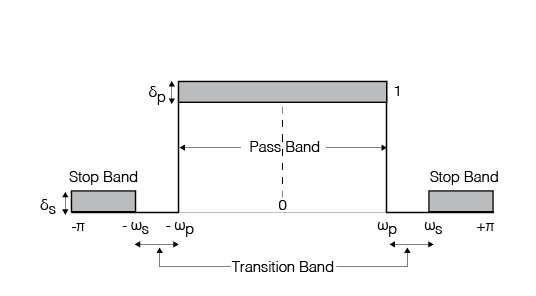
\includegraphics[width = 75mm, scale = 3]{low_pass_real.png}
\caption{Frequency Response of a Real Low-Pass Filter}
\label{fig:low_pass_real}
\end{figure}	 

Here, $\omega_p$ is known as the passband edge and $\omega_s$ is known as the stopband edge. The passband tolerance gives an upper limit on how much variance is allowed in our frequency response in the passband. Likewise, the stopband tolerance gives an upper limit on how much variance is allowed in our frequency response in the stopband. \smallskip

As engineers, our main objective is moving as close to the ideal filter as possible. For this, we need $\delta_p, \delta_s$ as small as possible and $\omega_s$ and $\omega_p$ as close as possible. An ideal filter has $\delta_s = 0$, $\delta_p = 0$ and $\omega_s = \omega_p$ \medskip

We shall mainly be dealing with four types of filters. They are:
\begin{enumerate}
    \item \textbf{Low Pass Filter}: This filter retains frequencies \textit{below} a certain threshold, and throws away the others.
    \item \textbf{High Pass Filter}: This filter retains frequencies \textit{above} a certain threshold and throws away the others.
    \item \textbf{Band Pass Filter}: This filter retains frequencies only in a certain band of frequencies, and throws away the others.
    \item \textbf{Band Stop Filter}: This filter blocks frequencies in a certain band of frequencies and retains all others.
\end{enumerate}

We have already discussed the response diagram of the low pass filter. The response diagrams for the other filters (with realistic specifications) are shown in Figure \ref{fig:high_pass_real} , \ref{fig:band_pass_real} and \ref{fig:band_stop_real}. Note: The response is only shown for positive frequencies as the graph is symmetric.

\begin{figure}[h!]
\centering
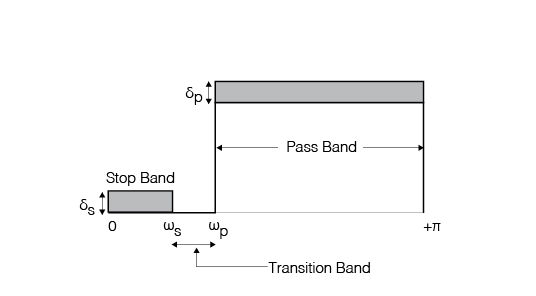
\includegraphics[width = 75mm, scale = 3]{high_pass_real.png}
\caption{Frequency Response of a Real High-Pass Filter}
\label{fig:high_pass_real}
\end{figure}	 

\begin{figure}[h!]
\centering
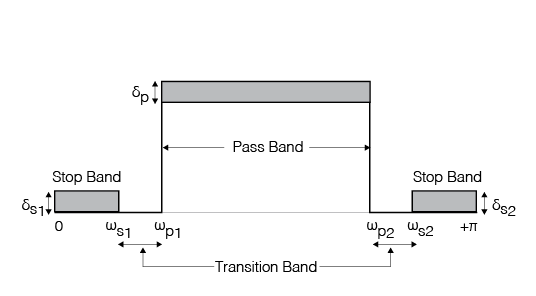
\includegraphics[width = 75mm, scale = 3]{band_pass_real.png}
\caption{Frequency Response of a Real Band-Pass Filter}
\label{fig:band_pass_real}
\end{figure}	 

\begin{figure}[h!]
\centering
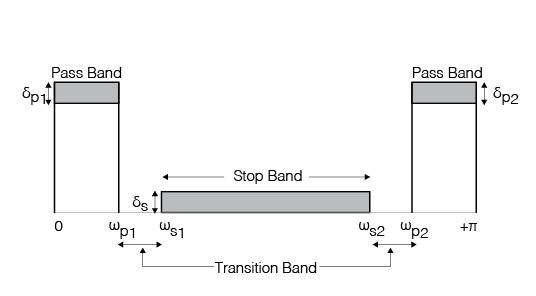
\includegraphics[width = 75mm, scale = 3]{band_stop_real.png}
\caption{Frequency Response for a Real Band-Stop Filter}
\label{fig:band_stop_real}
\end{figure}	 

Essentially, we have two choices for designing filters. We can have a filter which has an infinite length impulse response. Such a filter is known as an \textbf{Infinite Impulse Response Filter (IIR Filter)}. The LCCDE characterising this system would be recursive. An IIR Filter would have both poles and zeroes. There is a problem with designing IIR filters though. If the poles of the system lie too close to the unit circle, numerical inaccuracies may cause them to migrate out of the unit circle and cause the filter to be unstable. \smallskip

The other type of filter is one which has a finite length impulse response. Such a filter is known as \textbf{Finite Impulse Response Filter (FIR Filter)}. The LCCDE characterising this system would be non-recursive. Unlike the IIR Filter, an FIR Filter would be unconditionally stable.  

\subsection{The Bilinear Transform}

The basic strategy for designing discrete-time filters will be to design a corresponding analog filter and somehow map this filter from the continuous time domain to the discrete time domain. Let us specify the details of this mapping. \smallskip

An analog filter in the continuous-time domain will be characterised by the system function $H_{\text{analog}}(s)$. Here, $s$ is the Laplace domain variable, the continuous-time analogue of $z$. To convert an analog filter to a discrete-time filter, we need to replace $s$ by a suitable function of $z$, in the system function $H_{\text{analog}}(s)$. Once we have done this, we get the system function $H(z)$ for the corresponding discrete-time filter. We have already explained how to implement a given system function $H(z)$. Hence, we now focus on this map from $s$ to $z$. \smallskip

We need the map from $s$ to $z$ to preserve rationality. This is essential for implementation of the system. A rational function in $s$ must be mapped to a rational function in $z$. This is only possible if $s$ is itself a rational function of $z$. \smallskip

The map must preserve stability of the system. We can comment on the stability of the systems be seeing how our required map maps the $s$ plane to the $z$ plane. For stability in the $z$ plane, we need $z^n$ to decay or $\abs{z} < 1$. Thus the stable region in the $z$ plane is the interior of the unit circle. In the $s$ plane, we want $e^{st}$ to decay. Consider that $s = \Sigma + j\Omega$. Then, 
\[
    e^{st} = e^{(\Sigma + j \Omega) \cdot t} = e^{\Sigma t} \cdot e^{j \Omega t}
\]
Thus, for $e^{st}$ to decay, we need $\Sigma < 0$ or $\Re{(s)} < 0$. Thus the stable region in the $s$ plane is the left half plane. Thus, our map must satisfy the following correspondences:
\begin{enumerate}
    \item The left half plane in the $s$ plane $\longleftrightarrow$ Interior of the unit circle in the $z$ plane
    \item The right half plane in the $s$ plane $\longleftrightarrow$ Exterior of the unit circle in the $z$ plane
    \item The imaginary axis in the $s$ plane $\longleftrightarrow$ The unit circle in the $z$ plane (or : when $s = j\Omega$, $\abs{z} = 1$)
\end{enumerate}

Also, when we move from $\Omega : -\infty$ to $\Omega : +\infty$ in the $s$ plane, we must move from $\omega = -\pi$ to $\omega = \pi$ in the $z$ plane. Thus, we also have the following correspondences:

\begin{enumerate}
    \item $\Omega = 0 \longleftrightarrow \omega = 0$
    \item $\Omega \rightarrow -\infty \longleftrightarrow \omega \rightarrow -\pi$ 
    \item $\Omega \rightarrow \infty \longleftrightarrow \omega \rightarrow \pi$ 
\end{enumerate}

We start off with the following idea:
\[
    z^{\frac{1}{2}} - z^{-\frac{1}{2}} = j \cdot 2 \sin{\frac{\omega}{2}} \quad \text{when } z = e^{j\omega}
\]

This satisfies a few of our required properties. When $z$ is on the unit circle ($z = e^{j\omega}$), $s$ is on the imaginary axis. However, this function isn't a rational function of $z$. Furthermore, it maps the unit circle only to the part of the imaginary axis restricted between $-2$ and $2$. But, we want the unit circle to be mapped to the \textit{entire} imaginary axis (as $\omega \in (-\pi, \pi) \rightarrow \Omega \in (-\infty, \infty)$). Let us consider the tangent function instead of the sine function, as the tangent function spans the entire real number axis. We must divide the above expression by cosine. This gives us the following map:

\[
    \boxed{s = \frac{1 - z^{-1}}{1 + z^{-1}}}
\]

This map is known as the \textbf{Bilinear Transform}. We shall be using this map. It is easy to verify that it satisfies all our requirements. To find the relation between the discrete-time frequency $\omega$ and the continuous-time frequency $\Omega$, we put $z = \exp(j\omega)$ and $s = j \Omega$. This gives us the following relation:
\[
    j\Omega = \frac{1 - e^{-j\omega}}{1 + e^{-j\omega}} = j \frac{\sin \frac{\omega}{2}}{\cos \frac{\omega}{2}}
\]
\[
    \therefore \boxed{\Omega = \tan \frac{\omega}{2}}
\]

Consider the frequency response for a low pass filter as shown below. When we apply the bilinear transform, we get the following transformations
\begin{itemize}
    \item $\pi \longmapsto \infty$
    \item $\omega_s \longmapsto \Omega_s$
    \item $\omega_p \longmapsto \Omega_p$
    \item $-\pi \longmapsto -\infty$
    \item $-\omega_s \longmapsto -\Omega_s$
    \item $-\omega_p \longmapsto -\Omega_p$
\end{itemize}

Also, the specifications of the filter are preserved upon applying the bilinear transform. That is, the passband and stopband tolerances are carried over directly from the discrete-time domain to the continuous-time domain. The frequency response for the corresponding analog filter is as follows. \medskip

\subsection{Design Strategy and Low-Pass Filter Design}

In this section, we lay down our strategy for designing a general discrete-time filter and start with designing Analog Low-Pass filters

\begin{steps}
    \item Convert the discrete time specifications to the corresponding analog filter specifications via the transformation $\Omega = \tan \ddfrac{\omega}{2}$.
    \item Suppose we have to design a low-pass filter, then we design the corresponding analog low-pass filter. If our original filter is not a low-pass filter, then we use analog frequency transformations to convert the analog filter to a corresponding analog low-pass filter. In any case, we will only be designing analog low-pass filters. For other filters, we look for an equivalent low-pass filter.
    \item Once we have designed an analog low-pass filter (which may correspond to any of the four filters), we have its system function $H_{\text{analog}}(s)$. We then use the bilinear transform $s = \frac{1-z^{-1}}{1+z^{-1}}$ to get the corresponding discrete-time system function $H_{\text{discrete}}(z)$.
    \item Finally, we can implement $H_{\text{discrete}}(z)$ using Direct Form I, Direct Form II, Cascade Form or Parallel Form.
\end{steps}

We now focus on designing an Analog Low-Pass Filter. Consider that the specifications of the filter are as follows:

\begin{itemize}
    \item Passband edge : $\Omega_p$
    \item Stopband edge : $\Omega_s$
    \item Passband tolerance : $\delta_p$
    \item Stopband tolerance : $\delta_s$
\end{itemize}

By ``designing'' an analog low-pass filter, we mean to find a function $H_{\text{L}}(s)$ such that when we substitute $s = j \Omega$, the magnitude of the resulting function,  $\abs{H_{\text{L}}(j \Omega)}$ obeys the above specifications. \smallskip

We can design different kinds of filters to satisfy these specifications. A standard way to classify these filters is to analyse how the function $\abs{H_{\text{L}}(s)}$ behaves in the passband and the stopband. We can have two kinds of variations for each bands - \textbf{monotonic} and \textbf{oscillatory}. These give rise to four different kinds of filters. We shall study them one by one.

\subsection{The Butterworth Filter}

The Butterworth filter has a monotonic passband and a monotonic stopband. Before designing the filter, we must understand what we require out of our filter function. The basic three requirements are that the filter function must be
\begin{enumerate}
    \item stable
    \item causal
    \item rational
\end{enumerate}

To design the filter according to the specifications, we are only concerned with the magnitude of $H_{\text{L}}(s)$. Consider that the filter function is $H_{\text{L}}(s)$. The frequency response is then given by substituting $s = j \Omega$. Thus, the frequency response is $H_{\text{L}}(j \Omega)$. We define the effective transfer magnitude function as $\abs{H_{\text{L}}(j\Omega)}^2 = H_{\text{L}}(j\Omega) \cdot \overline{H_{\text{L}}(j\Omega)}$. If the coefficients of $H_{\text{L}}(s)$ are real, then we have that $\overline{H_{\text{L}}(j \Omega)} = H_{\text{L}}( -j \Omega)$. Extending this to all $s$, we define the Magnitude Analog function as $H_{\text{L}}(s) \cdot H_{\text{L}}(-s)$. \smallskip

For the magnitude analog function, for every pole/zero at $s=s_0$, we also have a pole/zero at $s = -s_0$. To ensure stability, we assign all the left-half plane poles to the function $H_{\text{L}}(s)$ and all the right-half plane poles to the function $H_{\text{L}}(-s)$. \medskip

To meet the required specifications, British engineer Stephen Butterworth came up with the following function:

\[
    H_{\text{L}}(s) \cdot H_{\text{L}}(-s) = \ddfrac{1}{1 + \left( \frac{s}{j \Omega_c} \right)^{2N}}
\]

On substituting $s = j\Omega$, we get the frequency response as

\[
    \ddfrac{1}{1 + \left( \frac{j \Omega}{j \Omega_c} \right)^{2N}} =  \boxed{\ddfrac{1}{1 + \left( \frac{\Omega}{\Omega_c} \right)^{2N}}}
\]

Here, $\Omega_c$ is the point where $\abs{H_{\text{L}}(j\Omega)}^2 = \frac{1}{2}$. Hence, $\Omega_c$ is called the \textit{half-power point}. $N$ corresponds to the rate at which the magnitude analog function drops. In practical scenarios, $N$ corresponds to the amount of resource we must invest to build the corresponding filter. Designing a Butterworth filter now reduces to choosing the correct $\Omega_c , N$ which meet the specifications. First, note that $\abs{H_{\text{L}}(j\Omega)}^2$ is always between $0$ and $1$. While, designing filters, we focus only on one side of the $\Omega$ axis, as the frequency response is symmetric. \medskip

Let us apply the condition for the passband. For the pass band, we want 
\[
    \ddfrac{1}{1 + \left( \frac{\Omega}{\Omega_c} \right)^{2N}} \geq (1-\delta_p)^2 \quad \text{all over the passband.}
\]

As the frequency response decreases with increasing $\Omega$, we essentially only want this condition to hold at the passband edge. If it is true at the passband edge, then it holds all over the passband. Thus,

\[
    \ddfrac{1}{1 + \left( \frac{\Omega_p}{\Omega_c} \right)^{2N}} \geq (1-\delta_p)^2
\]
\[
    \ddfrac{1}{(1-\delta_p)^2} \geq 1 + \left( \frac{\Omega}{\Omega_c} \right)^{2N} \quad \text{or} \quad \left( \frac{\Omega_p}{\Omega_c} \right)^{2N} \leq \frac{1}{(1-\delta_p)^2} - 1
\]
We denote $\frac{1}{(1-\delta_p)^2} - 1$ as $D_p$ ($D_p \geq 0$). Hence, we get:
\[
    \boxed{\left( \frac{\Omega_c}{\Omega_p} \right)^{2N} \geq \frac{1}{D_p}}
\] \medskip

Using similar arguments, for the stopband, we get
\[
   \ddfrac{1}{1 + \left( \frac{\Omega_s}{\Omega_c} \right)^{2N}} \leq \delta^2_s \quad \text{or} \quad \left( \frac{\Omega_s}{\Omega_c} \right)^{2N} \geq \frac{1}{\delta^2_s} - 1
\]
We denote $\frac{1}{\delta^2_s} - 1$ as $D_s$ ($D_s \geq 0$). Hence, we get 
\[
     \boxed{\left( \frac{\Omega_s}{\Omega_c} \right)^{2N} \geq D_s}
\]  

Multiplying the two inequalities, we get
\[
    \left( \frac{\Omega_s}{\Omega_p} \right)^{2N} \geq \frac{D_s}{D_p}
\]

Taking $\log$ on both sides, we get
\[
    \boxed{N \geq \frac{\log \left( \frac{D_s}{D_p}\right)^{\nicefrac{1}{2}}}{\log \left( \frac{\Omega_s}{\Omega_p}\right)}}
\]

This is the design condition for $N$. $N$ is also known as the filter order. To find the minimum order required, we can use the ceiling function.
\[
    N_{\text{min}} = \ceil[\Bigg]{\frac{\log \left( \frac{D_s}{D_p}\right)^{\nicefrac{1}{2}}}{\log \left( \frac{\Omega_s}{\Omega_p}\right)}}
\]

We now determine $\Omega_c$. From the two inequalities mentioned above, we can conclude the following result. 
\[
    \boxed{\frac{\Omega_p}{D_p^{\nicefrac{1}{2N}}} \leq \Omega_c \leq \frac{\Omega_s}{D_s^{\nicefrac{1}{2N}}}}
\]
This gives us a design condition for $\Omega_c$ given a particular $N$. Note: If we keep $\Omega_c$ closer to $\Omega_p$, then we are \textit{over-designing} the stopband and vice-versa. Thus, we can choose the position of $\Omega_c$ according to our needs. \smallskip

We now consider the function for all $s$ as follows
\[
    H_{\text{L}}(s) \cdot H_{\text{L}}(-s) = \ddfrac{1}{1 + \left( \frac{s}{j \Omega_c} \right)^{2N}}
\]

Note that this function has no non-trivial zeroes. Let us look for the poles. If $s$ is a pole then, the denominator must be zero. Therefore, 
\[
    1 + \left( \frac{s}{j \Omega_c} \right)^{2N} = 0 \implies \left( \frac{s}{j \Omega_c} \right)^{2N} = -1 = e^{j(2k+1)\pi}
\]
\[
    \therefore \frac{s}{j\Omega_c} = e^{j(2k+1)\pi}
\]
Thus, the poles are given by:
\[
    \boxed{s_k = j\Omega_c \cdot \exp{\left\{j \left(\frac{\pi}{2N} + \frac{k\pi}{N}\right)\right\}}}
\]  

Thus, all poles are on a circle centred at the origin having a radius of $\Omega_c$. We can show that the poles corresponding to $k = 0, \ldots , N-1$ are the left-half plane poles. Also, if $N$ is even, then we have that the poles corresponding to $k = 0 , \ldots , \frac{N}{2} - 1$ are complex conjugates of those corresponding to $k = \frac{N}{2} , \ldots , N-1$. If $N$ is odd, then there is a real pole at $-\pi$ and the others occur as complex conjugates. Hence, the poles always occur as complex conjugates and the function has real coefficients. We can thus construct our analog system function as:
\[
    H_{\text{L}}(s) = \frac{\kappa}{(s-s_1)(s-s_2) \ldots (s-s_N)}
\]
where $s_1, \ldots s_N$ are the left-half plane poles and $\kappa$ is a constant. We additionally need that $H_{\text{L}}(0) = 1$. Hence, 
\[
    H_{\text{L}}(0) = \frac{\kappa}{(-1)^N \prod\limits_{i=1}^{N} s_i} = 1
\]
Note: the indices $i$ and $k$ are different (shifted by one, to be precise). It is not to difficult to show that the denominator is $\Omega_c^N$ (Hint: The phases average out to $\pi$ and the magnitude of every pole is $\Omega_c$). Thus, we have $\kappa = \Omega_c^N$. Hence, our final analog system function is:
\[
    \boxed{H_{\text{L}}(s) = \frac{\Omega_c^N}{\prod\limits_{i = 1}^{N} (s - s_i)}}
\]
Finally, we use the Bilinear Transform on the above function to obtain our discrete-time system for the given low pass filter. Hence, this completes our analysis of the Butterworth Filter.

\subsection{The Chebyshev Filter}

\subsubsection{Chebyshev Polynomials}

The idea of Chebyshev polynomials arises from multi-angle trigonometric identities. Consider the following identities:
\begin{itemize}
    \item $\cos 2\theta = 2 \cos^2 \theta - 1$
    \item $\cos 3\theta = 4 \cos^3 \theta - 3 \cos \theta$
    \item $\cos 4 \theta = 8 \cos^4 \theta - 8 \cos^2 \theta + 1$
\end{itemize}

In general, $\cos N \theta = T_N(\cos \theta)$, where $T_N(\cdot)$ is a polynomial. These polynomials are known as \textbf{Chebyshev polynomials (of the first kind)}. For $x$, we define the $N^{\text{th}}$ Chebyshev polynomial as
\[
    T_N(x) = 
    \begin{cases}
    
    \cos (N \arccos x) & \text{if} \; \abs{x} \leq 1 \\
    \cosh (N \arccosh x) & \text{if} \; x \geq 1 \\
    (-1)^N \cosh (N \arccosh (-x) ) & \text{if} \; x \leq -1
    
    
    \end{cases}
\]

\textit{Properties.} Following are some properties of the Chebyshev polynomials.

\begin{enumerate}
    \item We can define the Chebyshev polynomials recursively via the relation $T_{N+1}(x) = 2x T_N(x) - T_{N-1}(x)$, with $T_0(x) = 1, T_1(x) = x$.
    \item The degree of $T_N(x)$ is $N$ and the leading coefficient is $2^{N-1}$.
    \item Odd and even powers never occur together in a Chebyshev polynomial
    \item The Chebyshev polynomials $T_N(\cdot)$ and $T_M(\cdot)$ satisfy $T_N(T_M(x)) = T_M(T_N(x)) = T_{NM}(x)$.
\end{enumerate}

\subsubsection{Designing the Chebyshev Filter}

The Chebyshev filter has an equiripple (oscillatory) passband and a monotonic stopband. For the Chebyshev filter, we define $H_{\text{L}}(s)$ such that
\[
    H_{\text{L}}(j\Omega) \cdot H_{\text{L}}(-j\Omega) = \ddfrac{1}{1 + \varepsilon^2 \cdot T_N^2 \left(\frac{\Omega}{\Omega_p}\right)}
\]  

Now, we apply the passband condition. 
\[
    \ddfrac{1}{1 + \varepsilon^2 \cdot T_N^2 \left(\frac{\Omega}{\Omega_p}\right)} \geq (1-\delta_p)^2 \quad \text{all over the passband}
\]
The magnitude of oscillations of the Chebyshev polynomials is $1$. Hence, this condition reduces to
\[
    \varepsilon^2 \leq \frac{1}{(1-\delta_p)^2} - 1 \implies \boxed{\varepsilon^2 \leq D_p}
\]

For $x > 1, T_N(x)$ is monotonically increasing. Hence, we apply the stopband condition only at the stopband edge. This gives us
\[
    \ddfrac{1}{1 + \varepsilon^2 \cdot T_N^2 \left(\frac{\Omega_s}{\Omega_p}\right)} \leq \delta_s^2
\]
Simplifying, we get
\[
    \varepsilon^2 \cdot T_N^2 \left( \frac{\Omega_s}{\Omega_p} \right) \geq \frac{1}{\delta_s^2} - 1 \implies \boxed{\varepsilon^2 \cdot T_N^2 \left( \frac{\Omega_s}{\Omega_p} \right) \geq D_s}
\]
Multiplying the two inequalities, we get
\[
    T_N \left( \frac{\Omega_s}{\Omega_p} \right) \geq \left( \frac{D_s}{D_p} \right)^{\nicefrac{1}{2}}
\]
Also, note that $\Omega_s \geq \Omega_p$, thus $\nicefrac{\Omega_s}{\Omega_p} \geq 1$. Therefore, we get
\[
    \boxed{N \geq \frac{\arccosh \left( \frac{D_s}{D_p}\right)^{\nicefrac{1}{2}}}{\arccosh \left( \frac{\Omega_s}{\Omega_p}\right)}}
\]

Note: This is the same expression as the Butterworth filter with the function $\log$ replaced by the function $\arccosh$. For a given set of specifications, we have that $N_B \geq N_C$ where $N_B$ is the filter order for the Butterworth filter and $N_C$ is the filter order for the Chebyshev filter (Hint: Compare the functions $\log$ and $\arccosh$). \smallskip

Now, we extend this function to all $s$, giving us
\[
    H_{\text{L}}(s) \cdot H_{\text{L}}(-s) = \ddfrac{1}{1 + \varepsilon^2 \cdot T_N^2 \left(\frac{s}{j \Omega_p}\right)}
\]

The poles are given by
\[
    T_N^2 \left( \frac{s}{j \Omega_p} \right) = - \frac{1}{\varepsilon^2} \implies T_N \left( \frac{s}{j \Omega_p} \right) = \pm \frac{j}{\varepsilon} \implies \cos \left(N \arccos \left( \frac{s}{j \Omega_p} \right) \right) = \pm \frac{j}{\varepsilon}
\]
Let $\arccos \left( \frac{s}{j \Omega_p} \right) = A_k + jB_k$ giving us $\cos(NA_k + jNB_k) = \pm \frac{j}{\varepsilon}$.

\[
    \cos NA_k \cos jNB_k - \sin NA_k \sin jNB_k = \pm \frac{j}{\varepsilon}
\]
\[
    \cos jNB_k = \cosh NB_k \quad ; \quad \sin jNB_k = j \sinh NB_k
\]
\[
    \therefore \cos NA_k \cosh NB_k - j \sin NA_k \sinh NB_k = \pm \frac{j}{\varepsilon}
\]
\[
    \cos NA_k \cosh NB_k = 0 \quad ; \quad \sin NA_k \sinh NB_k = \pm \frac{1}{\varepsilon}
\]
\[
    \therefore \cos NA_k = 0 \implies \boxed{A_k = \frac{(2k+1) \pi}{2N}} 
\]
\[
    A_k = \frac{(2k+1) \pi}{2N} \implies \sin NA_k = \pm 1 \implies \sinh NB_k = \pm \frac{1}{\varepsilon}
\]
Consider $B_k$ to be positive, giving us $B_k = \frac{1}{N} \arcsinh \frac{1}{\varepsilon} $. 
\[
    \therefore \frac{s_k}{j \Omega_p} = \cos ( A_k + j B_k ) = \cos A_k \cosh B_k - j \sin A_k \sinh B_k
\]
\[
    \therefore \boxed{s_k = \Omega_p \sin A_k \sinh B_k + j \Omega_p \cos A_k \cosh B_k} = \Sigma_k + j \Omega_k
\]
\[
    \Sigma_k = (\Omega_p \sinh B_k) \cdot \sin A_k \quad ; \quad \Omega_k = (\Omega_p \cosh B_k) \cdot \cos A_k
\]
\[
    \therefore \boxed{\left( \frac{\Sigma_k}{\sinh B_k} \right)^2 +  \left( \frac{\Omega_k}{\cosh B_k} \right)^2 = \Omega_p^2} \quad \text{using} \; \sin^2 A_k + \cos^2 A_k = 1
\]

Thus, the poles of the system lie on an ellipse with major axis along imaginary axis and minor axis along real axis. Consider that $s_1 , \ldots s_N$ are the poles in the left-half plane. Thus, we construct $H_{\text{L}}(s)$ as follows
\[  
    H_{\text{L}}(s) = \frac{\kappa}{(s-s_1)(s-s_2) \ldots (s-s_N)}
\]
To find the constant, we use the value of $H_{\text{L}}(0)$.
\begin{case}
    \item $N$ is even. In this case, we have $T_N^2(0) = 1$. Thus, 
    \[
        \frac{\kappa}{\prod\limits_{i=1}^{N} (-s_i)} = \frac{1}{\sqrt{1 + \varepsilon^2}}
    \]  
    We find $\kappa_{\text{even}}$ from here. 
    \item $N$ is odd. In this case, we have $T_N^2(0) = 0$. Thus,
    \[
         \frac{\kappa}{\prod\limits_{i=1}^{N} (-s_i)} = 1
    \]
    We find $\kappa_{\text{odd}}$ from here.
\end{case}

Finally, we define 
\[
    H_{\text{L}}(s) = \frac{\kappa}{\prod\limits_{i=1}^{N} (s-s_i)}
\]
where $\kappa$ is defined as 
\[
    \kappa = 
    \begin{cases}
    \kappa_{\text{even}} & N \text{ is even}\\
    \kappa_{\text{odd}} & N \text{ is odd}\\
    \end{cases}
\]

Finally, we apply the Bilinear Transform which gives us our discrete-time function. \medskip

We shall not be discussing the remaining two types of filters as their analysis is fairly involved. The filter with a monotonic passband and equiripple stopband is called an \textbf{Inverse Chebyshev Filter} or a \textbf{Chebyshev Type II Filter}. The filter with both bands equiripple is called an \textbf{Elliptic Filter} or a \textbf{Cauer Filter} or a \textbf{Zolotarev Filter}. The frequency responses for the four types of Low-Pass Filters is as shown in Figure \ref{fig:freq_rep}.

\begin{figure}[h!]
\centering
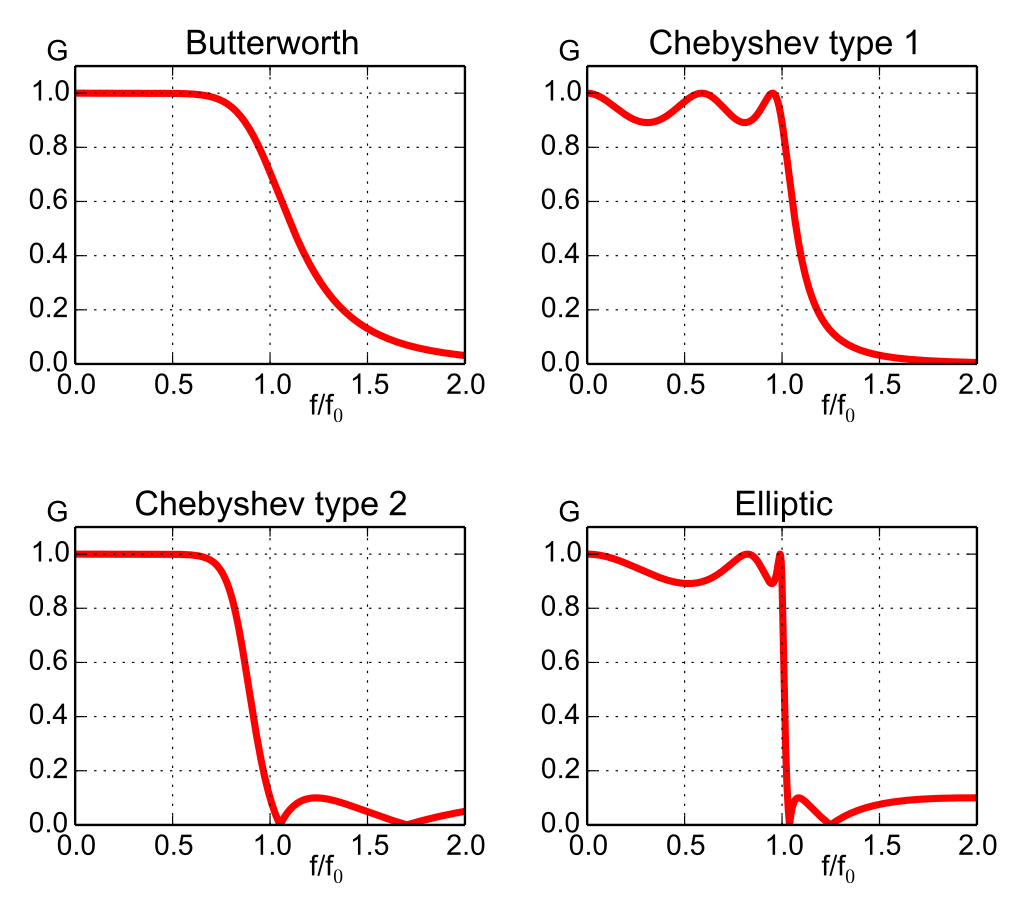
\includegraphics[width = 75mm, scale = 3]{frequency_responses.png}
\caption{Frequency responses of the four types of filters. [\textit{Image Source: Wikipedia}]}
\label{fig:freq_rep}
\end{figure}	 

\subsection{Analog Frequency Transformations}

So far, we have only designed the analog low-pass filter. To design the other three types of filters, we use analog frequency transformations. We denote the low-pass filter $s$ variable as $s_L$ and the general filter $s$ variable as $s$. A frequency transformation is then a function which maps a function of $s$ to $s_L$ or $F(s) \longmapsto s_L$. Again, we require this map to map the imaginary axis to the imaginary axis, left-half plane to the left-half plane, right-half plane to the right-half plane and it should preserve rationality. We sequentially these transformations for all three of the other filters.

\subsection{High Pass Filter}

To convert the high-pass filter to a low-pass filter, we use the following map (verify that it is indeed valid):
\[
    s_L = \frac{\Omega_h}{s}
\]  
where $\Omega_h$ is a constant. Substituting $s = j\Omega$ and $s_L = j \Omega_L$, we get the relation:
\[
    \boxed{\Omega_L = - \frac{\Omega_h}{\Omega}}
\]

We can see that as $\Omega$ moves from $0^+$ to $+\infty$, $\Omega_L$ moves from $-\infty$ to $0^-$ and as $\Omega$ moves from $-\infty$ to $0^-$, $\Omega_L$ moves from $0^+$ to $+\infty$. Thus, the passband region of the low-pass filter is the stopband region of the high-pass filter and vice versa. We have converted our high pass filter into a low pass filter. We now focus on only one side of the frequency spectrum (as the map is an odd map). The other filter characteristics - namely, the passband and stopband tolerances remain the same. The point $\Omega_p$ in the high-pass filter is mapped to the point $\Omega_{p_L}$ in the low-pass filter. By convention, we choose $\Omega_h = \Omega_p$. This gives us the passband edge in the low-pass filter to be $\Omega_{p_L} = \abs{- \frac{\Omega_h}{\Omega_p}} = 1$. Thus, we wish to design a low-pass filter having passband and stopband tolerances as $\delta_s, \delta_p$ (same as the high-pass filter) and having passband edge $1$ and stopband edge $\frac{\Omega_p}{\Omega_s}$ (Note: $\Omega_s < \Omega_p$ as these are specified for a high-pass filter). Once we design this filter, we get its system function $H_{\text{L}}(s_L)$. We then use $s_L= \frac{\Omega_p}{s}$ to find $H_{\text{H}}(s)$. We can then use the bilinear transform and implement the high pass filter.

\subsection{Bandpass Filter}

To convert the bandpass filter to a low pass filter, we use the following map (verify that it is indeed valid) :

\[
    s_L = \frac{s^2 + \Omega_0^2}{B s}
\]

where $\Omega_0$ and $B$ are constants. Substituting $s = j\Omega$ and $s_L = j \Omega_L$, we get the relation 
\[
    \boxed{\Omega_L = \frac{\Omega^2 - \Omega_0^2}{B \Omega}}
\]

Note:
\[
    \frac{d \Omega_L}{d \Omega} = \frac{1}{B} + \frac{\Omega_0^2}{B \Omega^2} > 0 \; \forall \; \Omega
\]

Thus, $\Omega_L$ is a monotonically increasing function of $\Omega$. As $\Omega$ moves from $0^{+}$ to $\Omega_{0}^{-}$, $\Omega_L$ moves from $-\infty$ to $0^{-}$. As $\Omega$ moves from $\Omega_{0}^{+}$ to $+\infty$, $\Omega_L$ moves from $0^{+}$ to $+\infty$. Also, $\Omega \mapsto \Omega_L$ is an odd mapping, hence we focus only on the positive side of $\Omega$ ($\Omega = 0$ is a point of singularity). Let the passband edges and stopband edges of the original bandpass filter be $\Omega_{p_1} , \Omega_{p_2} , \Omega_{s_1}$ and $\Omega_{s_2}$. We choose $\Omega_o$ to be somewhere in between $\Omega_{p_1}$ and $\Omega_{p_2}$. This allows the maps of the passband edges ($\Omega_{Lp_1}$ and $\Omega_{Lp_2}$) to be on opposite sides of $\Omega_L =0$. For convenience, we want these points to be exactly negative of each other. Hence, 
\[
    \Omega_{Lp_1} = -\Omega_{Lp_2} \implies \frac{\Omega_{p_1}^2 - \Omega_0^2}{B \Omega_{p_1}} = \frac{\Omega_{p_2}^2 - \Omega_0^2}{- B \Omega_{p_2}}
\]
\[
    \therefore \boxed{\Omega_0^2 = \Omega_{p_1} \cdot \Omega_{p_2}}
\]

For this value of $\Omega_0$, we are ensured that $\Omega_{p_1}$ and $\Omega_{p_2}$ are mapped to mutually negative points. Now, the constant $B$ only helps us to \textit{scale}. We use this constant ingeniously to make our passband edge equal to $1$ in the low-pass filter. That is, $\Omega_{p_1}$ maps to $-1$ and $\Omega_{p_2}$ maps to $+1$. This gives us,
\[
    \boxed{B = \Omega_{p_2} - \Omega_{p_1}}
\]

Thus, $B$ is the bandpass width of the filter. With these constants, we have the following maps from $\Omega$ to $\Omega_L$. 

\begin{itemize}
    \item $0 \longmapsto -\infty$
    \item $\Omega_{s_1} \longmapsto \Omega_{Ls_1}$
    \item $\Omega_{p_1} \longmapsto -1$
    \item $\Omega_0 \longmapsto 0$
    \item $\Omega_{p_2} \longmapsto +1$
    \item $\Omega_{s_2} \longmapsto \Omega_{Ls_2}$
    \item $+\infty \longmapsto +\infty$
\end{itemize}

A stopband from $0$ to $\Omega_{s_1}$ in the bandpass filter corresponds to a stopband from $-\infty$ to $\Omega_{Ls_1}$ in the transformed filter. A passband from $\Omega_{p_1}$ to $\Omega_{p_2}$ in the bandpass filter corresponds to a passband from $-1$ to $+1$ in the transformed filter. A stopband from $\Omega_{s_2}$ to $+\infty$ in the bandpass filter corresponds to a stopband from $\Omega_{Ls_2}$ to $+\infty$ in the transformed filter. Hence, the transformed filter is indeed a low-pass filter. However, the stopband edges on the positive and negative side ($\Omega_{Ls_2}$ and $\Omega_{Ls_1}$ respectively) may not be equal and opposite. Hence, we choose the more `stringent' of the two edges, that is, one which gives a smaller transition band. Thus, using the map mentioned with the mentioned values of $\Omega_0$ and $B$, gives us a low-pass filter having the following specifications :

\begin{enumerate}
    \item Passband edge : $1$
    \item Stopband edge : $\min \left\{ \abs{\Omega_{Ls_1}} , \abs{\Omega_{Ls_2}}\right\}$
    \item Passband and Stopband Tolerances and their nature (monotonic or equiripple) same as the original Bandpass Filter
\end{enumerate}

We then design a low-pass filter with these specifications, using the Butterworth/Chebyshev/Inverse Chebyshev/Elliptic Approximations. This gives us the low-pass system function $H_L(s_L)$. We then substitute $s_L = (s^2 + \Omega_o^2) \cdot (Bs)^{-1}$ with the required values of $\Omega_o$ and $B$ to get the corresponding bandpass function $H_{BP}(s)$. We then use the bilinear transform to get the corresponding discrete time system function, which we can implement.

\subsection{Bandstop Filter}

The map for a bandstop filter is the reciprocal of the map for a bandpass filter. Thus, we have 
\[
    s_L = \frac{Bs}{s^2 + \Omega_0^2}
\]

Substituting $s = j\Omega$ and $s_L = j \Omega_L$ gives us the relation
\[
    \Omega_L = \frac{B\Omega}{\Omega_0^2 - \Omega^2}
\]

While this map appears to be similar to the one for a bandpass filter, the corresponding frequency transformation is quite different. Note :
\[
    \frac{d\Omega_L}{d\Omega} = B \frac{\Omega_0^2 + \Omega^2}{(\Omega_0^2 - \Omega^2)^2}
\]

Thus, the derivative is positive for all $\Omega \neq \Omega_0$. At $\Omega_0$, the derivative diverges, as does $\Omega_L$. There is an infinite jump at the point $\Omega = \Omega_0$ (a point of singularity). We only focus on the positive region of $\Omega$. The region between $0$ and $\Omega_0$ on the $\Omega$ axis is mapped to the region between $0$ and $+\infty$ on the $\Omega_L$ axis (in the same order). The region between $\Omega_0$ and $+\infty$ on the $\Omega$ axis is mapped to the region between $-\infty$ and $0$ on the $\Omega_L$ axis (in the same order). In short as $\Omega$ increases from $0$ to $\Omega_0$, $\Omega_L$ increases from $0$ to $+\infty$. When $\Omega$ crosses the point $\Omega_0$, $\Omega_L$ `jumps' from $+\infty$ to $-\infty$. Then, as $\Omega$ increases from $\Omega_0$ to $+\infty$, $\Omega_L$ increases from $-\infty$ to $0$. \medskip

Like before, we want the passband edges to map to mutually negative points. This gives us essentially the same equation. Thus, $\Omega_0 = \sqrt{\Omega_{p_1} \cdot \Omega_{p_2}}$. We also make these edges to be $\pm 1$, giving us $B = \Omega_{p_2} - \Omega_{p_1}$. Like before, we use the more stringent stopband edge. Using these values of $\Omega_0$ and $B$, we get a low-pass filter with the following specifications:

\begin{enumerate}
    \item Passband edge : $1$
    \item Stopband edge : $\min \left\{ \abs{\Omega_{Ls_1}} , \abs{\Omega_{Ls_2}}\right\}$
    \item Passband and Stopband Tolerances and their nature (monotonic or equiripple) same as the original Bandpass Filter
\end{enumerate}

We then design a low-pass filter with these specifications, using the Butterworth/Chebyshev/Inverse Chebyshev/Elliptic Approximations. This gives us the low-pass system function $H_L(s_L)$. We then substitute $s_L =  (Bs) \cdot (s^2 + \Omega_0^2)^{-1}$ with the required values of $\Omega_0$ and $B$ to get the corresponding bandstop function $H_{BS}(s)$. We then use the bilinear transform to get the corresponding discrete time system function, which we can implement.

\section{Finite Impulse Response Filter Design}

\subsection{Linear Phase Response}

We now move to designing FIR Filters. An FIR Filter has two significant advantages. 
\begin{enumerate}
    \item It is unconditionally stable. 
    \item It has a better phase response than an IIR Filter.
\end{enumerate}

The first point makes sense as a finite length impulse response will certainly be absolutely summable. What about the second point? We first talk about the ideal, most desirable phase response (the phase response of an ideal filter). We categorise the phase response of an ideal filter as \textbf{Linear Phase}. We first demonstrate this idea in the continuous-time domain. Consider the a sinusoid $A_0 \cos (\Omega_0 t + \phi_0)$. A linear phase response is one which adds a linear phase term to the argument of the sinusoid. That is, this sinusoid is replaced by $A_0 \cos (\Omega_0 t + \Omega_0 \tau + \phi_0) = A_0 \cos (\Omega_0 (t + \tau) + \phi_0)$. This is equivalent to shifting the sinusoid by $\tau$ units of time. The important point is that this shift is \textit{independent} of the frequency $\Omega_0$. Linear phase is special as all sinusoids are shifted equally on the $t$-axis. For a discrete-time system with linear phase, the frequency response is given as 
\[
    H(\omega) = H_R(\omega) \cdot e^{j \Phi(\omega)} \quad ; \; H_R(\omega) \geq 0 \; \forall \; \omega \quad \Phi(\omega) = \omega \tau \; \text{where} \; \tau \; \text{is preferably an integer}
\]

Here, $H_R(\omega)$ is the magnitude response and $\Phi(\omega)$ is the phase response. We first deal with the continuous-time case. Here, the frequency response would be 
\[
    H_{\text{analog}}(\Omega) = H_R(\Omega) \cdot e^{j \Omega \tau} \quad H_R(\Omega) \geq 0 \; \forall \; \Omega
\]

However, we shall permit $H_R(\Omega)$ to be negative (as long as it is real). Thus, for $H_R(\Omega) \in \mathbb{R} \; \forall \; \Omega$, $H_R(\Omega) \cdot \exp (j \Omega \tau)$ represents \textbf{pseudo-linear phase}. We add the prefix `pseudo' as a negative magnitude response would add a phase change of $\pi$. Hence, a pseudo-linear phase response would show jumps of $\pi$ at some places. \medskip

The discrete-time version of pseudo-linear phase is given by
\[
    H(\omega) = H_R(\omega) \cdot e^{j \omega \tau} \quad \tau \in \frac{\mathbb{Z}}{2} \quad \text{or,} \; \tau \; \text{is a multiple of half}
\]

Let $h[n]$ be the impulse response, obtained by the Inverse DTFT of $H(\omega)$. We could regard $h[n]$ as samples of $h(t)$, being sampled at the integers, where $h(t)$ is the Inverse Continuous-Time Fourier Transform of the analogous system function $H_A(\Omega)$. We denote the magnitude response as $H_R(\Omega)$ and its inverse continuous-time Fourier transform as $h_R(t)$. Note that $h_R(t)$ will be a real and even function if and only if $H_R(\Omega)$ is a real and even function. We have the relation :
\[
    H_R(\Omega) = H_A(\Omega) \cdot e^{-j \Omega \tau} \implies h_R(t) = h(t - \tau)
\]

Hence, $-\tau$ is a point of symmetry in $h(t)$. If $\tau$ is an integer, then we can choose the point of symmetry as one of the samples and then take an equal number of samples on either side of the point of symmetry, giving us an odd number of total samples. If $\tau$ is a half-integer, then we choose an equal number of samples on either side of the point of symmetry, the first ones being at a distance of half each. This gives us an even number of total samples. If $\tau$ were an integer, the DTFT would be of the form:
\[
    H_R(\omega) \cdot e^{-j\omega D}
\]
where $H_R(\omega)$ is real and even. Similarly, if $\tau$ were a half integer, the DTFT would be of the form:
\[
    H_R(\omega) \cdot e^{-j \omega \left(D - \frac{1}{2} \right)}
\]

Similar arguments apply for real and odd signals. Here, the DTFT would be of the form 
\[
    j \cdot H_R(\omega) \cdot e^{-j\omega D}
\]

where $H_R(\omega)$ is real and odd. This is also a form of pseudo-linear phase where $j H_R(\omega)$ can contribute a phase change of $\frac{\pi}{2}$ or $-\frac{\pi}{2}$. 

\subsection{Truncation and Windowing}

The problem of filter design is essentially to approximate the (infinitely non-causal, unstable, irrational) ideal filter by a (causal, stable, rational) discrete-time system - a real filter. This problem is similar to representing an irrational number (say $\pi$) in a calculator or a computer. This is done by truncating and rounding off the decimal expansion of $\pi$. $3.14159 \cdots$ is often truncated and rounded off as $3.142$. A similar approach is applied to FIR Filter Design. Recall that the impulse response for the ideal filter is given by

\[
    h_{\text{ideal}} [n] = 
    \begin{cases}
        \ddfrac{\sin \omega_c n}{\pi n} & \text{if} \; n \neq 0 \\
        \ddfrac{\omega_c}{\pi} & \text{if} \; n = 0
    \end{cases}
\]

We will now truncate this sequence up to a desired length in order to design an FIR Filter. While truncating, we wish to keep symmetry/anti-symmetry intact to retain pseudo-linear phase. We then perform a generalised ``rounding off'' to the truncated response. This is done by multiplying the truncated response by an appropriate sequence. This sequence is known as a \textbf{Window Sequence} and this process is called windowing. \medskip

While retaining an odd number of samples, we consider zero to be one of the samples and collect an equal number of samples on either side of zero. Consider for example that we wish to retain $21$ samples in the impulse response of the ideal filter. This is naturally done by retaining the samples from $-10$ to $+10$. There are two reasons to do this:
\begin{enumerate}
    \item These central $21$ samples have the highest magnitude and thus contribute the most to the response
    \item Retaining samples from $-10$ to $+10$ allows us to retain symmetry.
\end{enumerate}

If we wish to retain an even number of samples, we then observe the underlying continuous time signal. That is, we consider 
\[
    \ddfrac{\sin \omega_c n}{\pi n} = \ddfrac{\sin \omega_c t}{\pi t} \quad \text{sampled at} \; t = n \; \text{(integers) for odd number of samples}
\]

For retaining an even number of samples, we retain two samples at $\frac{1}{2}$ units on either side of zero. Then, we take an equal number of on either side of these two samples at a distance of one unit each. For example, for retaining $20$ samples, we sample at $-9 \frac{1}{2} , - 8 \frac{1}{2} \cdots - \frac{1}{2} , \frac{1}{2} \cdots 8 \frac{1}{2} , 9 \frac{1}{2}$. \medskip

Truncating a sequence from $-N$ to $+N$ is equivalent to multiplying this sequence with $1$ from $-N$ to $+N$ and $0$ elsewhere. The process of windowing allows us to modify exactly how we multiply or modify this truncated part. A window sequence allows us flexibility to modify and change the chopped/truncated sequence according to our needs. Following are some common examples of windows :

\begin{enumerate}
    \item \textbf{Rectangular Window.} This window sequence is $1$ between $-N$ to $+N$ and zero everywhere else. Multiplication by a rectangular window is equivalent to a simple truncation of the sequence. We represent this window sequence graphically as follows:
    
    \item \textbf{Triangular Window.} This window is represented as follows. There is a linear decay in magnitude about the point of symmetry. 
    
    \item \textbf{Cosine Window.} This is as shown
\end{enumerate}

Consider any general window sequence $v[n]$. A window sequence must satisfy the following conditions
\begin{enumerate}
    \item $v[n]$ must be symmetric (to maintain symmetry/anti-symmetry of the response)
    \item $v[n]$ must be time-limited (as we need a finite impulse response)
\end{enumerate}

For a given window sequence $v[n]$, the truncated response is $h_{\text{tr}}[n] = h_{\text{ideal}}[n] \cdot v[n]$. However, the truncated response is still non-causal. But since it is now finite, we can make it causal by shifting or delaying the sequence by an appropriate number of samples. This delayed, causal sequence is the impulse response of the FIR Filter and is denoted as $h_{\text{FIR}}[n]$. \medskip

Let the DTFT of $h_{\text{ideal}}[n]$ be $H_{\text{ideal}}(\omega)$ and the DTFT of $v[n]$ be $V(\omega)$. The DTFT of $h_{\text{tr}}[n]$ is then given by (recall that this would be a \textit{periodic convolution} of the two DTFT's)
\[
    H_{\text{TR}}(\omega) = \frac{1}{2\pi} \int_{-\pi}^{\pi} H_{\text{ideal}}(\lambda) \cdot V(\omega - \lambda) d\lambda
\]

Let us first deal with a rectangular window. The DTFT of a rectangular window ($H_{\text{R}}(\omega)$) from $-N$ to $+N$ is given by 
\[
    H_{\text{R}}(\omega) = \sum_{n = -N}^{+N} e^{-j \omega n}
\]

This can be simplified using the formula for the sum of a geometric progression.
\[
    \therefore H_{\text{R}}(\omega) = e^{j \omega N} \left( \ddfrac{1 - e^{-j\omega (2N+1)}}{1 - e^{j\omega}} \right)
\]
On simplifying, we get 
\[
    H_{\text{R}}(\omega) = \ddfrac{\sin \frac{2N+1}{2} \omega}{\sin \frac{\omega}{2}}
\]

The graph for $H_{\text{R}}(\omega)$ is shown in Figure. Although we derived this for a rectangular window, such a graph is typical of many window sequences. $H_{\text{R}}(\omega)$ has one main-lobe centered around $\omega = 0$ and has side-lobes on either side. The most significant side-lobe is the one nearest to the main-lobe. Now, let us find $H_{\text{TR}}(\omega)$. An intuitive way to do this is by moving the shape of $H_{\text{R}}(\omega)$ from left to right, scaling it by the value of the ideal frequency response at every point and then finding the total area. We divide our study into five critical regions: 
\begin{enumerate}
    \item In the first region, the main-lobe of $H_{\text{R}}(\omega)$ is centered far at the left (starting from $-\pi$). In this case, the main-lobe remains outside the passband and is multiplied by zero, nullifying its contribution. Hence, all the area is contributed only by the side-lobes. Further, as the main-lobe moves rightward, side-lobes of alternating positive and negative area move into and out of the passband. Hence, the response here will be an oscillating response with a very small average value (roughly zero). This region represents the first stopband.
    \item In the second region, the main-lobe is just at the edge of the passband. As the main-lobe enters the passband, a large positive area is contributed. This causes the response to rise from a low value to a high value. This region represents the first transition band.
    \item In the third region, the main-lobe is completely within the passband and moves from the left passband edge to the right one. Here, the average value of the response does not change as the most significant contribution (the one from the main-lobe) remains intact. However, the movement of the side-lobes causes oscillation about this high value. This region represents the passband.
    \item In the fourth region, the main-lobe is just at the edge of the passband. As the main-lobe leaves the passband, a large positive area is subtracted from the response. This causes the response to fall back to a low value from a high value. This region represents the second transition band.
    \item In the fifth region, the main-lobe of $H_{\text{R}}(\omega)$ is centered far at the right (ending at $\pi$). In this case, the main-lobe remains outside the passband and is multiplied by zero, nullifying its contribution. Hence, all the area is contributed only by the side-lobes. Further, as the main-lobe moves rightward, side-lobes of alternating positive and negative area move into and out of the passband. Hence, the response here will be an oscillating response with a very small average value (roughly zero). This region represents the second stopband.
\end{enumerate}

Overall, the truncated response is shown in Figure \ref{fig:trunc_resp}. 

\begin{figure}[!h]
    \centering
    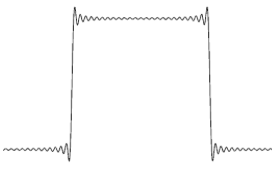
\includegraphics[scale=0.5]{trunc_resp.png}
    \caption{Truncated Response for a Rectangular window.}
    \label{fig:trunc_resp}
\end{figure}

A few important points:

\begin{itemize}
    \item The width of the transition band is determined by the width of the main-lobe
    \item The extent of oscillations in the passband and stopband are equal as they are caused by the same side-lobes
    \item The extent of oscillations in the passband and stopband are determined by the area of the most significant side-lobe.
\end{itemize}

Let us find the main-lobe width of the rectangular window. The main-lobe width will be the separation between the first two nulls in $\abs{V_{\text{R}}(\omega)}$. This is given by 
\[
    \sin \frac{2N + 1}{2} \omega = 0 \implies \omega = \pm \frac{2 \pi}{2N + 1}
\]
Thus, the main-lobe width is given by 
\[
    \Delta_{\text{R}} = \frac{4 \pi}{2N + 1}
\]

To get closer to an ideal filter, we must reduce both the main-lobe width as well as the side-lobe area. Clearly, we can reduce the main-lobe width by increasing $N$ (while we've only shown this for the rectangular window, this is true, in general, for all windows). Consider that $N \rightarrow \infty$. In this case, the main-lobe width, $\Delta_{\text{R}}$ tends to zero. However, it can be shown that the side-lobe area tends to a \textit{non-zero constant}. Thus, there is a \textit{fundamental limit} for the side-lobe area which we cannot improve upon even by investing infinite resources. Thus, the ripples in the passband and stopband are lower bounded. This is a manifestation of the \textbf{Gibb's Phenomenon of Fourier Series}. \medskip

Another interesting thing to note is that the main-lobe width and side-lobe area are in conflict with one another. We want the truncated frequency response to be concentrated around the zero frequency. However, we also want to minimise the resources invested - or reduce the length of the truncated response. These two objectives are in fundamental conflict with one another. We cannot make something narrow in both the time domain and the frequency domain. This is an interesting manifestation of the \textbf{Uncertainty principle}. The uncertainty principle limits or forbids the simultaneous localisation in both the time and frequency domain. \medskip

Consider that we have fixed $N$. This gives a fundamental bound on the spread around zero frequency. We can ``implement'' this spread by either increasing the main-lobe width or increasing the side-lobe area. Hence, there is a fundamental compromise between these two quantities. The obvious question that arises - is there a window which optimises both these parameters for a given $N$? Before we deal with this question, let us list down a few important windows. Here, we consider the window to be zero in all regions where the window is not specified.

\begin{enumerate}
    \item \textbf{Rectangular Window}. This is sometimes also known as the \textbf{boxcar} or the \textbf{Dirichlet window}. This window sequence is defined by 
    \[
        v[n] = 1 \quad 0 \leq n \leq N 
    \]
    
    \item \textbf{Triangular Window}. The triangular window is a symmetric window with its peak at $N \over 2$ and linearly decaying to either side. This window sequence is given by 
    \[
        v[n] =  1 - \abs{\frac{2n - N}{L}} \quad 0 \leq n \leq N 
    \]
    
    where $L$ can be $N$, $N+1$ or $N+2$. For $L=N$, the window is also known as the \textbf{Bartlett window} or the \textbf{Fejér window}.
    
    \item \textbf{Parzen Window}. This is also known as the \textbf{de la Vallée Poussin Window}. Define $L = N+1$. We define this sequence between $-L \over 2$ and $L \over 2$ as follows
    \[
        v[n] = 
        \begin{cases}
        1 - 6 \left( \frac{2n}{L} \right)^2 \left( 1 - \frac{2 \abs{n}}{L} \right) & 0 \leq \abs{n} \leq \frac{L}{4} \\
        2\left( 1 - \frac{2 \abs{n}}{L} \right)^3 & \frac{L}{4} \leq \abs{n} \leq \frac{L}{2}
        \end{cases}
    \]
    
    \item \textbf{Welch Window}. The Welch window consists of a single parabolic section. It is defined as 
    \[
        v[n] = 1 - \left( \frac{2n - N}{N} \right)^2 \quad 0 \leq n \leq N 
    \]
    
    \item \textbf{Power of Sine Windows}. A general power of sine window is given as 
    \[
        v[n] = \sin^\alpha \left( \ddfrac{\pi n}{N} \right) \quad 0 \leq n \leq N 
    \]
    
    For $\alpha = 0$, we get the \textbf{Rectangular window}. For $\alpha = 1$ we get the \textbf{Sine Window} and for $\alpha = 2$ we get the \textbf{Hann Window}.
    
    \item \textbf{Hamming Window.} This is also known as a raised cosine window (as the average of the cosine is slightly above zero). It is defined as
    \[
        v[n] = \ddfrac{25}{46} - \ddfrac{21}{46} \cdot \cos \left( \ddfrac{2\pi n}{N} \right) \quad 0 \leq n \leq N 
    \]
    
    \item \textbf{Blackman Window}. The Blackman window can be considered to be a \textit{refinement} of the Hamming window, as it adds a harmonic to the sequence, The Blackman window is defined as
    \[
        v[n] = a_0 - a_1 \cos \left( \frac{2\pi n}{N} \right) + a_2 \cos \left( \frac{4\pi n}{N} \right) \quad 0 \leq n \leq N
    \]
    
    With $a_0 = \frac{1 - \alpha}{2}, a_1 = \frac{1}{2}$ and $a_2 = \frac{\alpha}{2}$. The exact Blackman window is defined with 
    \[
        a_0 = \frac{7938}{18608}; \quad a_1 = \frac{9240}{18608}; \quad a_2 = \frac{1430}{18608}
    \]
    A good approximation to this uses $\alpha = 0.16$.
    
    \item \textbf{Nuttall Window}. For four constants $a_0, a_1, a_2$ and $a_3$ such that $a_0 + a_1 + a_2 + a_3 = 1$, we define the window 
    \[
        v[n] = a_0 - a_1 \cos \left( \frac{2\pi n}{N} \right) + a_2 \cos \left( \frac{4\pi n}{N} \right) - a_3 \cos \left( \frac{6\pi n}{N} \right) \quad 0 \leq n \leq N
    \]
    For different values of the constants, we get the following three windows 
    \begin{enumerate}
        \item \textbf{Nuttall Window}
        \item \textbf{Blackman-Nuttall Window}
        \item \textbf{Blackman-Harris Window }
    \end{enumerate}
    
    \item \textbf{Tukey Window}. The Tukey window is also known as a cosine-tapered window. It is a combination of the rectangular window and the Hann window. Define $L = N+1$. Consider an $\alpha$ between $0$ and $1$. We define the Tukey window as 
    \[
        v[n] = 
        \begin{cases}
        \frac{1}{2} \left[ 1 - \cos \left( \frac{2\pi n}{\alpha L}\right) \right] & 0 \leq n < \frac{\alpha L}{2} \\
        1 & \frac{\alpha L}{2} \leq n \leq \frac{N}{2} \\
        v[N-n] & \frac{N}{2} \leq n \leq N
        \end{cases}
    \]
    
    For $\alpha =0$, this becomes a rectangular window and for $\alpha=1$, this becomes a Hann window.
\end{enumerate}

\subsection{The Kaiser Window}

We talked about the `compromise' between the main-lobe width and the side-lobe area. The window which provides the optimal compromise is known as the \textbf{Kaiser Window} or the \textbf{Kaiser-Bessel Window}. This window is based on the Bessel-function (specifically, the zeroth-order modified Bessel function of the first kind). We define this function as follows
\[
    I_0(x) = 1 + \sum_{l =1}^{\infty} \left[ \ddfrac{\left( \nicefrac{x}{2}\right)^l}{l!}\right]^2
\]
The Kaiser window is then defined as
\[
    v[n] = \frac{I_0 \left[ \beta\sqrt{ 1 - \left( \frac{n - \alpha}{\alpha} \right)^2}\right]}{I_0[\beta]} \quad 0 \leq n \leq N
\]

where $\beta > 0$ is the shape parameter and $\alpha = \frac{N}{2}$. For $\beta=0$, the Kaiser window reduces to the rectangular window. A smaller $\beta$ corresponds to a smaller main-lobe. By increasing $N$, we can modulate the transition band without affecting the ripple. \medskip

Determination of the parameters $\beta$ and $N$ is done via empirical equations. Empirical equations do not have any analytic or theoretical background but are derived through observations and curve-fitting. Consider that we wish to design a low-pass filter having passband and stopband edges $\omega_p$ and $\omega_s$. Define $\Delta \omega = \omega_s - \omega_p$. Let the passband and stopband tolerances be $\delta_p$ and $\delta_s$. Note that the passband and stopband ripple values are equal. Hence, a filter designed by this method will have equal tolerances. Hence, we choose the more stringent of the two tolerances. Define $\delta = \min \{ \abs{\delta_p} , \abs{\delta_s} \}$. We define 
\[
    A = -20 \logten \delta
\]
Based on the value of $A$, we choose $\beta$ as 
\[
    \beta = 
    \begin{cases}
        0.1102 (A - 8.7) & A > 50 \\
        0.5842 (A - 21)^{0.4} + 0.07886(A-21) & 21 \leq A \leq 50 \\
        0 & A < 21
    \end{cases}
\]

For given values of $A$ and $\Delta \omega$, we choose $N$ as
\[
    N = \frac{A - 8}{2.285 \Delta \omega}
\]

This completes the design of the required Kaiser window. Let us consider a numerical example. \smallskip

\textbf{Example.} Consider a low-pass filter having the following specifications:
\begin{itemize}
    \item $\omega_p = 0.4 \pi$
    \item $\omega_s = 0.6 \pi$
    \item $\delta_p = 0.01$
    \item $\delta_s = 0.001$
\end{itemize}

For this filter, we compute $\delta = 0.001$ and $\Delta \omega = 0.2 \pi$. Further, we can compute $A$ to be 
\[
    A = -20 \logten (0.001) = 60
\]

As $A > 50$, we compute $\beta$ as 
\[
    \beta = 0.1102 ( 60 - 8.7 ) = 5.653 
\]

Further, using $A$ and $\Delta \omega$, we compute $N$ as 
\[
    N = \frac{60 - 8}{2.285 \times 0.2 \pi} = 37
\]

This completes the design of the respective Kaiser window. We can also compute $\alpha = \frac{37}{2} = 18.5$. Further, we can approximate the cutoff frequency as 
\[
    \omega_c = \frac{\omega_s + \omega_p}{2} = 0.5 \pi
\]

This gives us the truncated response 
\[
    h_{\text{tr}}[n] = 
    \begin{cases}
    \ddfrac{\sin 0.5 \pi (n - 18.5)}{\pi (n- 18.5)} \cdot \ddfrac{I_0 \left[ 5.653 \sqrt{ 1 - \left( \frac{n - 18.5}{18.5} \right)^2}\right]}{I_0[5.653]} & 0 \leq n \leq 37 \\
    0 & \text{otherwise}
    \end{cases}
\]

\subsection{Lattice Structures}

\subsubsection{The Lattice Equations}

We had previously discussed realisation of systems through the direct forms, the cascade form and the parallel form. Another important method of system realisation is through lattice structures or through lattice synthesis. We generally use the term lattice to denote a regular periodic repetition of some fundamental constituent or unit. The meaning here is the same. \medskip

We define a single unit in a lattice structure as a two input - two output unit. This unit is shown in Figure \ref{fig:lattice_1}. 

\begin{figure}[!h]
  \centering
  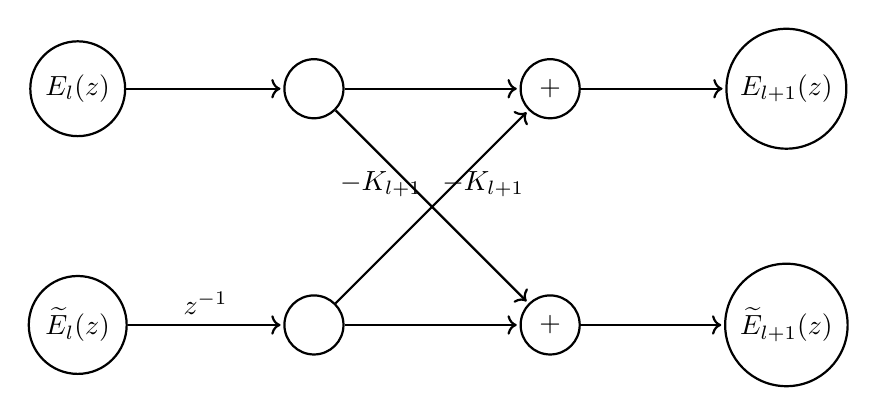
\begin{tikzpicture}[shorten >=1pt,node distance=3cm,on grid,auto]
    \tikzstyle{state}=[shape=circle,thick,draw,minimum size=0.75cm]
    \tikzstyle{process}=[shape=rectangle,thick,draw,minimum size=0.75cm]

    \node[state] (A0) {$E_l(z)$};
    \node[state, below of=A0] (B0) {$\widetilde{E}_{l}(z)$};
    \node[state, right of=A0] (A1) {};
    \node[state, right of=B0] (B1) {};
    \node[state, right of=A1] (A2) {$+$};
    \node[state, right of=B1] (B2) {$+$};
    \node[state, right of=A2] (A3) {$E_{l+1}(z)$};
    \node[state, right of=B2] (B3) {$\widetilde{E}_{l+1}(z)$};
    
    \path[->, draw, thick]
    (A0) edge node {} (A1)
    (B0) edge node {$z^{-1}$} (B1)
    (A1) edge node {$-K_{l+1}$} (B2)
    (B1) edge node {$\quad \quad -K_{l+1}$} (A2)
    (A1) edge node {} (A2)
    (B1) edge node {} (B2)
    (A2) edge node {} (A3)
    (B2) edge node {} (B3)
    
	;
  \end{tikzpicture}
  \caption{A Basic Unit of a Lattice Structure. $K_{l+1}$ is a constant, and $l$ denotes the stage of the lattice.} 
  \label{fig:lattice_1}
\end{figure}

This graph can be equivalently represented via the following two equations
\[
    E_{l+1}(z) = E_l(z) - K_{l+1} z^{-1} \widetilde{E}_{l}(z)
\]
\[
    \widetilde{E}_{l+1}(z) = z^{-1} \widetilde{E}_{l}(z) - K_{l+1} E_l(z)
\]

We make the first two inputs equal. That is, $E_0(z) = \widetilde{E}_{0}(z)$. Further, we divide all terms by $E_0(z) ( = \widetilde{E}_0(z))$. This gives us 
\[
    A_l(z) = \frac{E_l(z)}{E_0(z)} ; \quad \widetilde{A}_{l}(z) = \frac{\widetilde{E}_{l}(z)}{\widetilde{E}_{0}(z)} 
\]

Thus, we get the equations 
\[
    A_{l+1}(z) = A_l(z) - K_{l+1} z^{-1} \widetilde{A}_{l}(z)
\]
\[
    \widetilde{A}_{l+1}(z) = z^{-1} \widetilde{A}_{l}(z) - K_{l+1} A_l(z)
\]

\begin{prop}
For $l \geq 1$, the terms $A_l(z)$ and $\widetilde{A}_{l}(z)$ are related as
\[  
    \widetilde{A}_{l}(z) = z^{-l} A_l(z^{-1}) 
\]  
\end{prop}
\begin{proof}
We prove this using mathematical induction. Let us first establish the basis. Clearly, $A_0(z) = 1$ and $\widetilde{A}_{0}(z) = 1$. Putting $l=0$ in the original equations, we get 
\[
    A_1(z) = 1 - K_1 z^{-1} ; \quad \widetilde{A}_{1}(z) = z^{-1} - K_1
\]
Thus, 
\[
    \widetilde{A}_{1}(z) = z^{-1} A_1(z^{-1}) 
\]

Now, let us assume that the proposition holds true for some $n$. Thus, we have 
\[
    \widetilde{A}_{n}(z) = z^{-n} A_n(z^{-1}) \quad \text{for some } n 
\]

Using the two equations, we have 
\[
    A_{n+1}(z) = A_n(z) - K_{n+1} z^{-1} \cdot z^{-n} A_n(z^{-1})
\]
\[
    \widetilde{A}_{n+1}(z) = z^{-1} \cdot z^{-n} A_n(z^{-1}) - K_{n+1} A_n(z)
\]

First, we replace $z$ by $z^{-1}$ in the first equation and then multiply by $z^{-(n+1)}$. On simplifying, we get 
\[
    \widetilde{A}_{n+1}(z) = z^{-(n+1)} A_{n+1}(z^{-1})
\]

Hence, the result follows from mathematical induction.
\end{proof}

\subsubsection{Realising FIR Systems via a Lattice Structure}

Consider an FIR system function given by 
\[
    H(z) = \sum_{m=0}^{N} b_m \cdot z^{-m}
\]

We use a $N$-stage lattice to realise this system. Further, we define $A_l$ and $\widetilde{A}_{l}$ as 
\[
    A_l(z) = \sum_{m=0}^{l} a_{l,m} \cdot z^{-m};\quad \widetilde{A}_{l}(z) = \sum_{m=0}^{l} a_{l,l-m} \cdot z^{-m}
\]

Also, we have the equation 
\[
    A_{l+1}(z) = A_l(z) - K_{l+1} z^{-1} \widetilde{A}_{l}(z)
\]
The maximum power of $z^{-1}$ in $A_l$ and $\widetilde{A}_{l}$ is $l$. Hence, we compare the coefficients of $z^{-(l+1)}$ on both sides. Thus, the coefficient of $z^{-(l+1)}$ in $A_{l+1}(z)$ is equal to $-K_{l+1}$ times the coefficient of $z^{-l}$ in $\widetilde{A}_{l}(z)$. Further, the coefficient of $z^{-l}$ in $\widetilde{A}_{l}(z)$ is equal to the coefficient of $z^0$ in $A_l(z)$. We can also prove that the coefficient of $z^0$ in $A_l(z)$ is $1$ for all $l$ (Hint: Use induction). Thus, we get 
\[
    \text{the coefficient of } z^{-(l+1)} \text{ in } A_{l+1}(z) = -K_{l+1}
\]

Let us now return our focus to the system function $H(z)$. We have 
\[
    H(z) = A_N(z) = \sum_{m=0}^{N} b_m \cdot z^{-m} ; \quad K_N = - b_N
\]

We use the method of \textit{Backward Recursion} to realise FIR systems. That is, we wish to obtain $A_l$ from $A_{l+1}$. We have 
\[
   A_{l+1}(z) = A_l(z) - K_{l+1} z^{-1} \widetilde{A}_{l}(z)
\]
Substituting the values of $A_l$ and $\widetilde{A}_{l}$, we have 
\[
    \sum_{m=0}^{l+1} a_{l+1,m} \cdot z^{-m} = \sum_{m=0}^{l} a_{l,m} \cdot z^{-m} - K_{l+1} \sum_{m=0}^{l} a_{l,l-m} \cdot z^{-(m+1)}
\]

Comparing coefficients for $m = 1, \ldots , l$, we get
\[
    a_{l+1,m} = a_{l,m} - K_{l+1} \cdot a_{l,l+1-m}
\]  

To construct backward recursion, we first replace $m$ by $l+1-m$ in the above equation. Then, we eliminate $a_{l,l+1-m}$. This gives us the following relation
\[
    \boxed{a_{l,m} = \frac{a_{l+1,m} + K_{l+1} \cdot a_{l+1, l+1-m}}{1 - K_{l+1}^2}}
\]

provided $K_{l+1}^2 \neq 1$. \medskip

For example, consider $l=4$. We know $a_{5,1} , a_{5,2} , a_{5,3}$ and $a_{5,4}$. Also, $K_5 = - a_{5,5}$. Thus we can find $a_{4,1}, a_{4,2} , a_{4,3}$ and $a_{4,4}$ via the following equations
\[
    a_{4,1} = \frac{a_{5,1} + K_5 \cdot a_{5,4}}{1 - K_5^2}
\]
\[
    a_{4,2} = \frac{a_{5,2} + K_5 \cdot a_{5,3}}{1 - K_5^2}
\]
\[
    a_{4,3} = \frac{a_{5,3} + K_5 \cdot a_{5,2}}{1 - K_5^2}
\]
\[
    a_{4,4} = \frac{a_{5,4} + K_5 \cdot a_{5,1}}{1 - K_5^2}
\]

Once, we have these coefficients, we can further proceed from $l=4$ to $l=3$ by using the coefficients $a_{4,1}, a_{4,2}$ and $a_{4,3}$ and setting $K_4 = - a_{4,4}$. Thus, we can go all the way up to $l=1$. \medskip

Note: This lattice structure only works when all the zeroes of the system are inside the unit circle. This is equivalent to saying that the modulus of $K$ at every stage must be strictly less than one. Let us demonstrate this via a numerical example. \medskip

\textbf{Example.} Consider that the system function of an FIR Filter is given by 
\[
    H(z) = 1 + \frac{3}{4}z^{-1} +\frac{1}{2}z^{-2} + \frac{1}{4} z^{-3}
\]

Here, the maximum power of $z^{-1}$ is $3$. Hence, we define $N=3$. We start with the last stage, that is, $l=2$. To find $K_3$, we have 
\[
    A_3(z) = H(z) = 1 + \frac{3}{4}z^{-1} +\frac{1}{2}z^{-2} + \frac{1}{4} z^{-3}
\]
Thus, we get 
\[
    \boxed{K_3 = - \frac{1}{4}}
\]
Now, to find $K_2$, we use the relation 
\[
    A_2(z) = \frac{A_3(z) + K_3 \cdot \widetilde{A}_{3}(z)}{1 - K_3^2}
\]
Thus, 
\[
    A_2(z) = \frac{16}{15} \cdot \left[ \left( 1 + \frac{3}{4}z^{-1} +\frac{1}{2}z^{-2} + \frac{1}{4} z^{-3}\right) - \frac{1}{4} \left( z^{-3} + \frac{3}{4}z^{-2} +\frac{1}{2}z^{-1} + \frac{1}{4}\right) \right]
\]
Simplifying, we get 
\[
    A_2(z) = 1 + \frac{2}{3} z^{-1} + \frac{1}{3} z^{-2}
\]
Thus, we get 
\[
    \boxed{K_2 = - \frac{1}{3}}
\]
Now, to find $K_1$, we use the relation
\[
    A_1(z) = \frac{A_2(z) + K_2 \cdot \widetilde{A}_{2}(z)}{1 - K_2^2}
\]  
Thus, 
\[
    A_1(z) = \frac{9}{8} \cdot \left[\left( 1 + \frac{2}{3} z^{-1} + \frac{1}{3} z^{-2}\right) - \frac{1}{3} \left(z^{-2} + \frac{2}{3} z^{-1} + \frac{1}{3} \right) \right]
\]
Simplifying, we get
\[
    A_1(z) = 1 + \frac{1}{2} z^{-1}
\]
Thus, we get 
\[
    \boxed{K_1 = - \frac{1}{2}}
\]
Also, we have $A_0(z) = 1$. The lattice realisation for this system is shown in Figure \ref{fig:lattice_ex}

\begin{figure}[h]
  \centering
  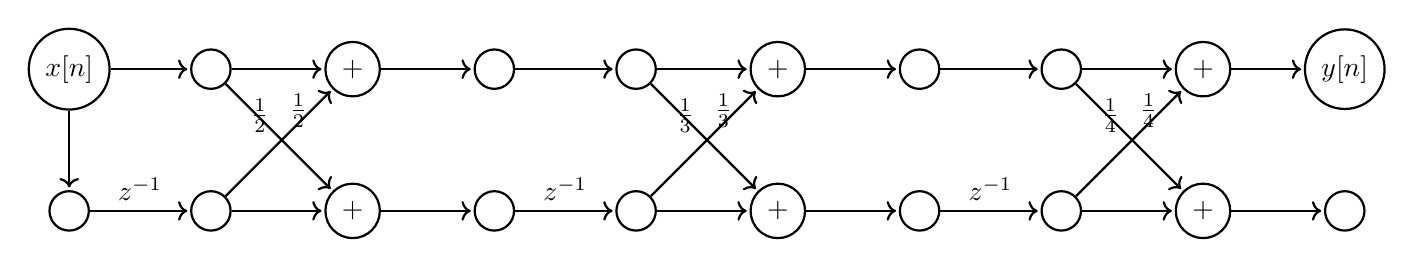
\begin{tikzpicture}[shorten >=1pt,node distance=1.8cm,on grid,auto]
    \tikzstyle{state}=[shape=circle,thick,draw,minimum size=0.50cm]
    \tikzstyle{process}=[shape=rectangle,thick,draw,minimum size=0.50cm]

    \node[state] (A0) {$x[n]$};
    \node[state, below of=A0] (B0) {};
    \node[state, right of=A0] (A1) {};
    \node[state, right of=B0] (B1) {};
    \node[state, right of=A1] (A2) {$+$};
    \node[state, right of=B1] (B2) {$+$};
    \node[state, right of=A2] (A3) {};
    \node[state, right of=B2] (B3) {};
    
    \node[state, right of=A3] (A11) {};
    \node[state, right of=B3] (B11) {};
    \node[state, right of=A11] (A12) {$+$};
    \node[state, right of=B11] (B12) {$+$};
    \node[state, right of=A12] (A13) {};
    \node[state, right of=B12] (B13) {};
    
    \node[state, right of=A13] (A21) {};
    \node[state, right of=B13] (B21) {};
    \node[state, right of=A21] (A22) {$+$};
    \node[state, right of=B21] (B22) {$+$};
    \node[state, right of=A22] (A23) {$y[n]$};
    \node[state, right of=B22] (B23) {};
    
    \path[->, draw, thick]
    (A0) edge node {} (A1)
    (A0) edge node {} (B0)
    (B0) edge node {$z^{-1}$} (B1)
    (A1) edge node {$\frac{1}{2}$} (B2)
    (B1) edge node {$\quad \frac{1}{2}$} (A2)
    (A1) edge node {} (A2)
    (B1) edge node {} (B2)
    (A2) edge node {} (A3)
    (B2) edge node {} (B3)
    
    (A3) edge node {} (A11)
    (B3) edge node {$z^{-1}$} (B11)
    (A11) edge node {$\frac{1}{3}$} (B12)
    (B11) edge node {$\quad \frac{1}{3}$} (A12)
    (A11) edge node {} (A12)
    (B11) edge node {} (B12)
    (A12) edge node {} (A13)
    (B12) edge node {} (B13)
    
    (A13) edge node {} (A21)
    (B13) edge node {$z^{-1}$} (B21)
    (A21) edge node {$\frac{1}{4}$} (B22)
    (B21) edge node {$\quad \frac{1}{4}$} (A22)
    (A21) edge node {} (A22)
    (B21) edge node {} (B22)
    (A22) edge node {} (A23)
    (B22) edge node {} (B23)

	;
  \end{tikzpicture}
  \caption{Lattice Realisation for the given problem.} 
  \label{fig:lattice_ex}
\end{figure}


\subsubsection{Generalising to IIR Systems}

Generalising this concept to IIR Systems requires a simple change of designation. We rearrange the first equation and keep the second equation intact. This gives us 
\[
    E_l(z) = E_{l+1}(z) + K_{l+1} \cdot z^{-1} \cdot \widetilde{E}_{l}(z)
\]
\[
    \widetilde{E}_{l+1}(z) = z^{-1} \widetilde{E}_{l}(z) - K_{l+1} E_l(z)
\]

In a sense, our inputs are now $E_N$ and $\widetilde{E}_0$. We represent this via the signal flow graph shown in Figure \ref{fig:lattice_2}

\begin{figure}[h]
  \centering
  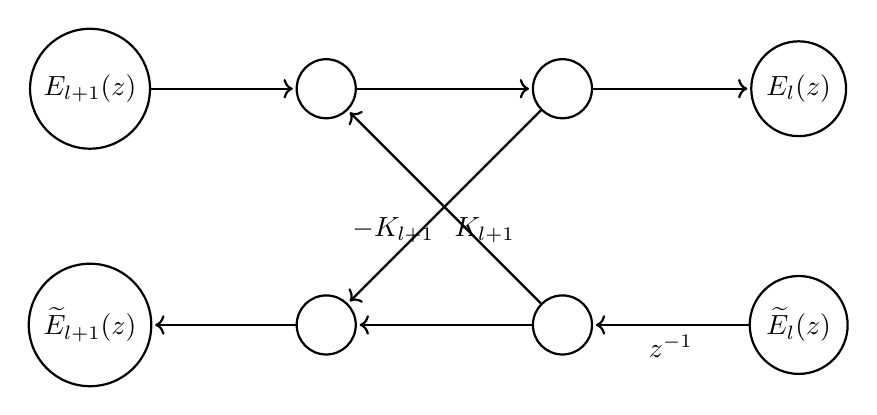
\begin{tikzpicture}[shorten >=1pt,node distance=3cm,on grid,auto]
    \tikzstyle{state}=[shape=circle,thick,draw,minimum size=0.75cm]
    \tikzstyle{process}=[shape=rectangle,thick,draw,minimum size=0.75cm]

    \node[state] (A0) {$E_{l+1}(z)$};
    \node[state, below of=A0] (B0) {$\widetilde{E}_{l+1}(z)$};
    \node[state, right of=A0] (A1) {};
    \node[state, right of=B0] (B1) {};
    \node[state, right of=A1] (A2) {};
    \node[state, right of=B1] (B2) {};
    \node[state, right of=A2] (A3) {$E_l(z)$};
    \node[state, right of=B2] (B3) {$\widetilde{E}_{l}(z)$};
    
    \path[->, draw, thick]
    (A0) edge node {} (A1)
    (B1) edge node {} (B0) 
    (B2) edge node {$\quad -K_{l+1}$} (A1)
    (A2) edge node {$K_{l+1}$} (B1)
    (A1) edge node {} (A2)
    (B2) edge node {} (B1)
    (A2) edge node {} (A3)
    (B3) edge node {$z^{-1}$} (B2)
    
	;
  \end{tikzpicture}
  \caption{Lattice Structure for IIR Systems} 
  \label{fig:lattice_2}
\end{figure}

For the sake of convenience, we mask all the connections shown and represent this unit as a single `black box' as shown in Figure \ref{fig:lattice_box}.

\begin{figure}[!h]
  \centering
  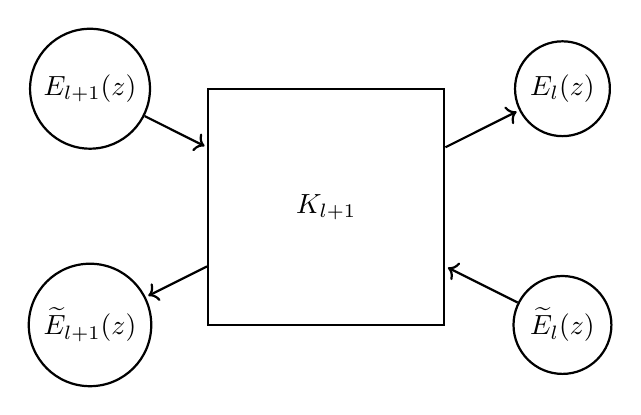
\begin{tikzpicture}[shorten >=1pt,node distance=3cm,on grid,auto]
    \tikzstyle{state}=[shape=circle,thick,draw,minimum size=0.75cm]
    \tikzstyle{process}=[shape=rectangle,thick,draw,minimum size=3cm]
    \tikzstyle{blank}=[shape=circle, minimum size=0.75cm]

    \node[state] (A0) {$E_{l+1}(z)$};
    \node[state, below of=A0] (B0) {$\widetilde{E}_{l+1}(z)$};
    \node[state, right=6cm of A0] (A1) {$E_l(z)$};
    \node[state, right=6cm of B0] (B1) {$\widetilde{E}_{l}(z)$};
    \node[blank, right of=A0] (X) {};
    \node[process, below=1.5cm of X] (Y) {$K_{l+1}$};
    
    \path[->, draw, thick]
    (A0) edge node {} (Y)
    (Y) edge node {} (A1)
    (B1) edge node {} (Y)
    (Y) edge node {} (B0)
    
	;
  \end{tikzpicture}
  \caption{Lattice Structure with a `Black Box'} 
  \label{fig:lattice_box}
\end{figure}

We can use this unit recursively to construct the signal flow graph as shown in Figure \ref{fig:lattice_iir} \medskip

\begin{figure}[!h]
  \centering
  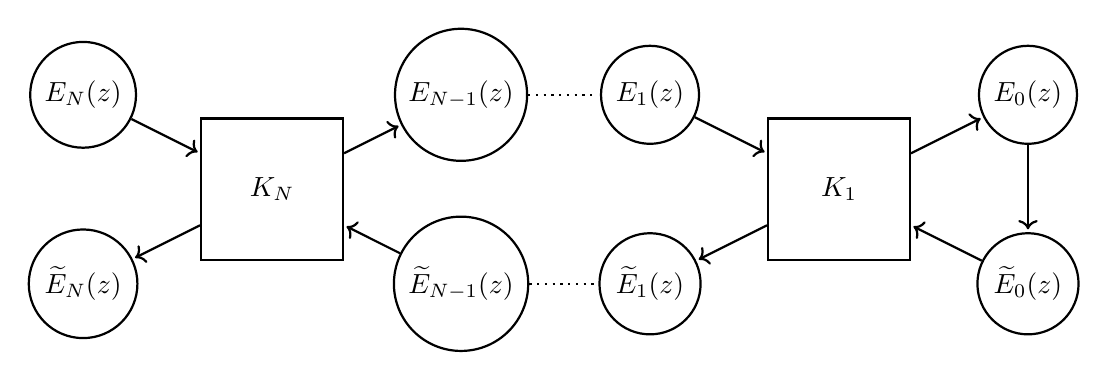
\begin{tikzpicture}[shorten >=1pt,node distance=2.4cm,on grid,auto]
    \tikzstyle{state}=[shape=circle,thick,draw,minimum size=0.75cm]
    \tikzstyle{process}=[shape=rectangle,thick,draw,minimum size=1.8cm]
    \tikzstyle{blank}=[shape=circle, minimum size=0.75cm]

    \node[state] (A0) {$E_{N}(z)$};
    \node[state, below of=A0] (B0) {$\widetilde{E}_{N}(z)$};
    \node[state, right=4.8cm of A0] (A1) {$E_{N-1}(z)$};
    \node[state, right=4.8cm of B0] (B1) {$\widetilde{E}_{N-1}(z)$};
    \node[blank, right of=A0] (X) {};
    \node[process, below=1.2cm of X] (Y) {$K_{N}$};
    \node[state, right of=A1] (A2) {$E_{1}(z)$};
    \node[state, below of=A2] (B2) {$\widetilde{E}_{1}(z)$};
    \node[state, right=4.8cm of A2] (A3) {$E_{0}(z)$};
    \node[state, right=4.8cm of B2] (B3) {$\widetilde{E}_{0}(z)$};
    \node[blank, right of=A2] (X1) {};
    \node[process, below=1.2cm of X1] (Y1) {$K_{1}$};
    
    \path[->, draw, thick]
    (A0) edge node {} (Y)
    (Y) edge node {} (A1)
    (B1) edge node {} (Y)
    (Y) edge node {} (B0)
    (A2) edge node {} (Y1)
    (Y1) edge node {} (A3)
    (B3) edge node {} (Y1)
    (Y1) edge node {} (B2)
    (A3) edge node {} (B3)
	;
	
	\draw[dotted, thick] (A1) -- (A2);
	\draw[dotted, thick] (B1) -- (B2);
	
  \end{tikzpicture}
  \caption{Lattice Structure for an IIR System} 
  \label{fig:lattice_iir}
\end{figure}

This type of recursive implementation can be used only for all-pole systems. For all-pole systems, the numerator of $H(z)$ is $1$ and we set the denominator = $A_N(z)$. For pole-zero systems, we use a modified structure known as a \textbf{Lattice-Ladder Structure}. A general lattice-ladder structure is shown in Figure \ref{fig:lattice_ladder}. \medskip

\begin{figure}[!h]
  \centering
  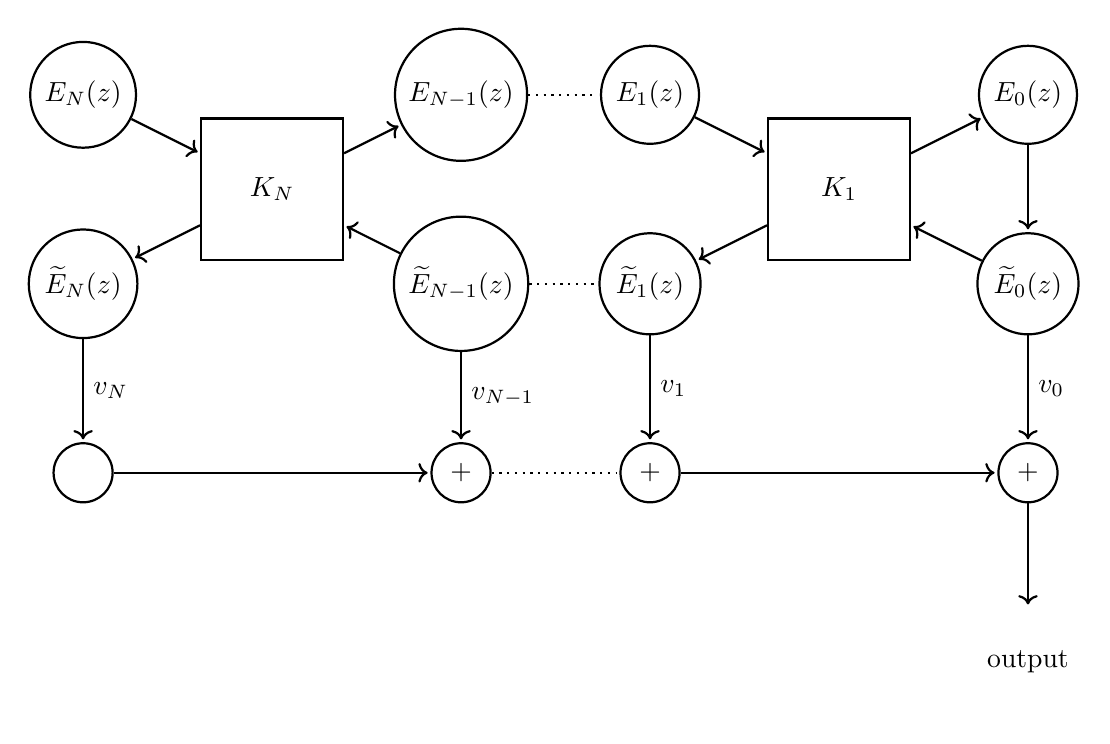
\begin{tikzpicture}[shorten >=1pt,node distance=2.4cm,on grid,auto]
    \tikzstyle{state}=[shape=circle,thick,draw,minimum size=0.75cm]
    \tikzstyle{process}=[shape=rectangle,thick,draw,minimum size=1.8cm]
    \tikzstyle{blank}=[shape=circle, minimum size=0.75cm]

    \node[state] (A0) {$E_{N}(z)$};
    \node[state, below of=A0] (B0) {$\widetilde{E}_{N}(z)$};
    \node[state, right=4.8cm of A0] (A1) {$E_{N-1}(z)$};
    \node[state, right=4.8cm of B0] (B1) {$\widetilde{E}_{N-1}(z)$};
    \node[blank, right of=A0] (X) {};
    \node[process, below=1.2cm of X] (Y) {$K_{N}$};
    \node[state, right of=A1] (A2) {$E_{1}(z)$};
    \node[state, below of=A2] (B2) {$\widetilde{E}_{1}(z)$};
    \node[state, right=4.8cm of A2] (A3) {$E_{0}(z)$};
    \node[state, right=4.8cm of B2] (B3) {$\widetilde{E}_{0}(z)$};
    \node[blank, right of=A2] (X1) {};
    \node[process, below=1.2cm of X1] (Y1) {$K_{1}$};
    \node[state, below of=B0] (C0) {};
    \node[state, right=4.8cm of C0] (C1) {$+$};
    \node[state, right of=C1] (C2) {$+$};
    \node[state, right=4.8cm of C2] (C3) {$+$};
    \node[blank, below of=C3] (D) {output};
    
    \path[->, draw, thick]
    (A0) edge node {} (Y)
    (Y) edge node {} (A1)
    (B1) edge node {} (Y)
    (Y) edge node {} (B0)
    (A2) edge node {} (Y1)
    (Y1) edge node {} (A3)
    (B3) edge node {} (Y1)
    (Y1) edge node {} (B2)
    (A3) edge node {} (B3)
    (B0) edge node {$v_N$} (C0)
    (C0) edge node {} (C1)
    (C2) edge node {} (C3)
    (C3) edge node {} (D)
    (B1) edge node {$v_{N-1}$} (C1)
    (B2) edge node {$v_1$} (C2)
    (B3) edge node {$v_0$} (C3)
    
	;
	
	\draw[dotted, thick] (A1) -- (A2);
	\draw[dotted, thick] (B1) -- (B2);
	\draw[dotted, thick] (C1) -- (C2);
	
  \end{tikzpicture}
  \caption{Lattice-Ladder Structure for an IIR System} 
  \label{fig:lattice_ladder}
\end{figure}

To find the coefficients $v_i$, we first define $C_M(z)$ to be the numerator of $H(z)$. We use the same method of backward recursion to find $C_{M-1}(z), \ldots , C_1(z)$ and $\widetilde{C}_{M-1}(z) , \ldots , \widetilde{C}_{1}(z)$. Then, we have the relation 
\[
    C_M(z) = \sum_{m=0}^{M} v_m \widetilde{C}_{m}(z)
\]  
From here, we can find the values of the constants $v_0 , \ldots , v_M$. Let us consider a numerical example. \medskip

\textbf{Example.} Consider the system function 
\[
    H(z) = \frac{1 + 2z^{-1} + 3z^{-2} + 2z^{-3}}{1 + 0.9z^{-1} - 0.8z^{-2} + 0.5z^{-3}}
\]
We have $N=3$ and $M=3$. We define $A_3(z) = 1 + 0.9z^{-1} - 0.8z^{-2} + 0.5z^{-3}$ and $C_3(z) =  1 + 2z^{-1} + 3z^{-2} + 2z^{-3}$. Using the same method as the previous example, we get 
\[
    \boxed{K_3(A) = -0.5; \; K_2(A) = 1.67; \; K_3(A) = -1.62}
\]
\[  
    K_3(C) = -2; \; K_2(C) = - \frac{1}{3}; \; K_1(C) = -0.75
\]
\[
    \widetilde{C}_{3}(z) = z^{-3} + 2z^{-2} + 3z^{-1} + 2; \; \widetilde{C}_{2}(z) = \frac{1}{3} + \frac{4}{3} z^{-1} + z^{-2}; \; \widetilde{C}_{1}(z) = \frac{3}{4} + z^{-1}
\]
Thus, we have 
\[
    1 + 2z^{-1} + 3z^{-2} + 2z^{-3} = v_0 + v_1 \cdot \widetilde{C}_{1}(z) + v_2 \cdot \widetilde{C}_{2}(z) + v_3 \cdot \widetilde{C}_{3}(z)
\]
On comparing the coefficients, we get 
\[
    \boxed{v_3 = 2; \; v_2 = -1; \; v_1 = - \frac{13}{4}; \; v_0 = - \frac{107}{48}}
\]

The realisation of this system is shown in Figure \ref{fig:lattice_ladder_ex}.

\begin{figure}[!h]
  \centering
  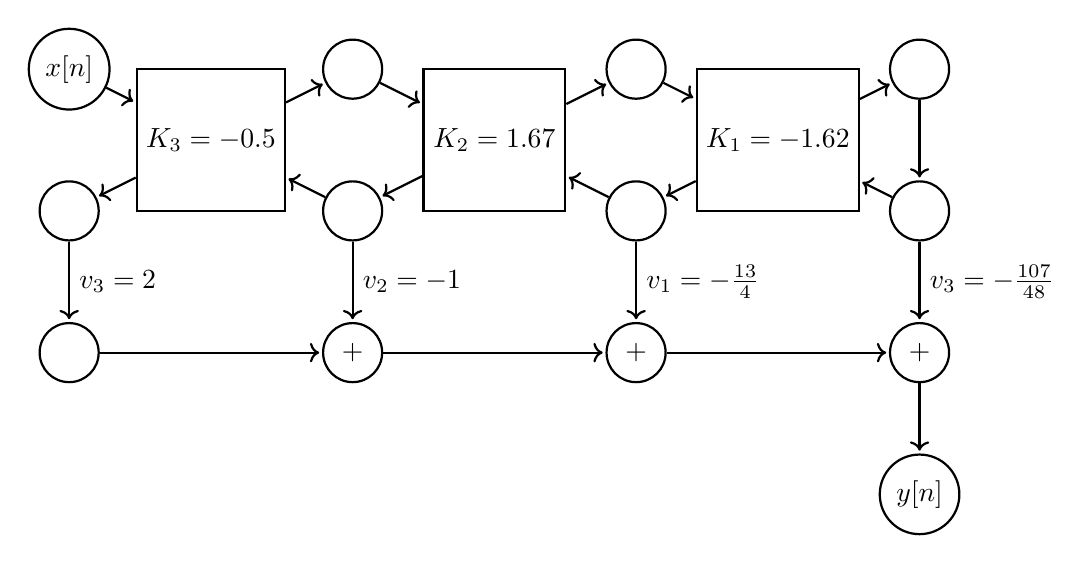
\begin{tikzpicture}[shorten >=1pt,node distance=1.8cm,on grid,auto]
    \tikzstyle{state}=[shape=circle,thick,draw,minimum size=0.75cm]
    \tikzstyle{process}=[shape=rectangle,thick,draw,minimum size=1.8cm]
    \tikzstyle{blank}=[shape=circle, minimum size=0.75cm]

    \node[state] (A0) {$x[n]$};
    \node[state, below of=A0] (B0) {};
    \node[state, right=3.6cm of A0] (A1) {};
    \node[state, right=3.6cm of B0] (B1) {};
    \node[blank, right of=A0] (X0) {};
    \node[process, below=0.9cm of X0] (Y0) {$K_3 = -0.5$};
    
    \node[state, right=3.6cm of A1] (A2) {};
    \node[state, right=3.6cm of B1] (B2) {};
    \node[blank, right of=A1] (X1) {};
    \node[process, below=0.9cm of X1] (Y1) {$K_2 = 1.67$};
  
    \node[state, right=3.6cm of A2] (A3) {};
    \node[state, right=3.6cm of B2] (B3) {};
    \node[blank, right of=A2] (X2) {};
    \node[process, below=0.9cm of X2] (Y2) {$K_1 = -1.62$};
    
    \node[state, below of=B0] (C0) {};
    \node[state, right=3.6cm of C0] (C1) {$+$};
    \node[state, right=3.6cm of C1] (C2) {$+$};
    \node[state, right=3.6cm of C2] (C3) {$+$};
    
    \node[state, below of=C3] (D) {$y[n]$};
    
    \path[->, draw, thick]
    (A0) edge node {} (Y0) 
    (Y0) edge node {} (A1)
    (Y0) edge node {} (B0)
    (B1) edge node {} (Y0)
    
    (A1) edge node {} (Y1) 
    (Y1) edge node {} (A2)
    (Y1) edge node {} (B1)
    (B2) edge node {} (Y1)
    
    (A2) edge node {} (Y2) 
    (Y2) edge node {} (A3)
    (Y2) edge node {} (B2)
    (B3) edge node {} (Y2)
    (A3) edge node {} (B3)
    
    (B0) edge node {$v_3 = 2$} (C0)
    (C0) edge node {} (C1)
    (B1) edge node {$v_2 = -1$} (C1)
    (C1) edge node {} (C2)
    (B2) edge node {$v_1 = -\frac{13}{4}$} (C2)
    (C2) edge node {} (C3)
    (B3) edge node {$v_3 = -\frac{107}{48}$} (C3) 
    (C3) edge node {} (D)
	;

  \end{tikzpicture}
  \caption{Lattice-Ladder Structure for the given IIR System.} 
  \label{fig:lattice_ladder_ex}
\end{figure}



\section{The Discrete Fourier Transform}

\subsection{Discretising the Frequency Axis}

So far, we have discretised \textit{time}. This was done so that we could work with analog signals on computers, store these signals etc. However, even after discretising time, we cannot work with the frequencies as they still form a continuum. To deal with this problem, we introduce the idea of discretising the \textit{frequency} axis as well. The obvious way to do this is to take the DTFT of a sampled sequence and sample the frequency axis of this DTFT. \medskip

Consider a sequence $x[n]$ which has a DTFT $X(\omega)$. No, we wish to discretise the $\omega$-axis. Consider that we retain only $N$ discrete points on the $\omega$-axis, located as follows. Here, it is convenient for us to take $\omega$ ranging from $0$ to $2\pi$ instead of $-\pi$ to $\pi$. We divide the interval $[0,2\pi]$ into $N$ sub-intervals and take one sample at the edge of each interval. This gives us the samples
\[
    \omega = \frac{2\pi}{N} k \quad k = 0, \ldots , N-1
\]
Now, to reconstruct a sequence from its DTFT, the integral in the inverse DTFT is replaced by a sum. This gives us a sequence 
\[
    \widetilde{x}[n] = \sum_{k=0}^{N-1} X\left( \frac{2\pi}{N}k \right) e^{j \left( \frac{2\pi}{N}kn \right)}
\]

Another way to construct the sequence $\widetilde{x}[n]$ is to use the `Dual' of the sampling theorem. For the original analog signal, we took the Fourier transform of the samples. We translated the spectrum in $-\pi$ to $\pi$ by every multiple of $2\pi$ and added all these translated spectra. For this case, we use a similar approach. The repeating interval (akin to the sampling interval) in this case would be 
\[
    \frac{2\pi}{\Delta\omega} = \frac{2\pi}{\nicefrac{2\pi}{N}} = N
\]


Thus, $\widetilde{x}[n]$ is obtained by translating $x[n]$ by every multiple of $N$ and adding all these together. Hence, we have 
\[
    \widetilde{x}[n] = \lambda_0 \sum_{r= -\infty}^{\infty} x[n + rN]
\]
We also allow for a constant of normalisation $\lambda_0$. 

Consider the sequence given by 
\[
    x[n] = \ldots  \mathbf{5} , 2 , 7 , 4 , 2 \ldots
\]
Here, the sequence $x[n]$ is zero everywhere else. The bold value indicates the zero index ($n=0$). Consider that we choose $N=3$. For this $N$, we can calculate $\widetilde{x}[n]$ using the above formula. $\widetilde{x}[n]$ turns out to be the sequence
\[
    \widetilde{x}[n] = \cdots 9, 4, 7, \mathbf{9}, 4, 7, 9, 4, 7, \cdots
\]

$\widetilde{x}[n]$ is periodic with period $3$. This is true in general as well. $\widetilde{x}[n]$, in general, will be periodic with period $N$. We can see this property from the original definition itself.
\[
    \widetilde{x}[n] = \lambda_0 \sum_{r= -\infty}^{\infty} x[n + rN]
\]
\[
    \widetilde{x}[n+N] = \lambda_0 \sum_{r= -\infty}^{\infty} x[n + (r+1)N] = \lambda_0 \sum_{r^{\prime}= -\infty}^{\infty} x[n + r^{\prime}N]
\]
\[
    \therefore \widetilde{x}[n+N] = \widetilde{x}[n]
\]

We define the \textbf{support} of a sequence as the extent of the sequence. That is, the support of a sequence is the range in which all the non-zero values of the sequence occur. An interesting thing to note is that when we used $N=3$ on the above sequence, the sequence $\widetilde{x}[n]$ which we obtained was ``corrupted'' or its values were different than the original sequence. This is due to \textbf{time-domain aliasing}. \medskip

If a sequence has an infinite support then aliasing is bound to occur. Consider a sequence $x[n]$ has a finite support. Without loss of generality, assume that this support is $0$ to $P-1$ (or $P$ samples). If we choose $N \geq P$, then $\widetilde{x}[n] = x[n]$ in the support of $x[n]$. That is, time-domain aliasing will not occur for $N \geq P$. This is because the translated samples do not overlap with the original samples. However, if we choose $N < P$, aliasing will occur as the translated samples overlap with the original ones. In the above example, we have $P=5$ and we chose $N$ as $3$, which is less than $5$. Hence, aliasing occurred. If we chose $N=5$, then this aliasing wouldn't have occurred. An interesting point: A sequence with finite support is equivalent to a band-limited signal. \medskip

\subsection{Formulating the Discrete Fourier Transform}

Consider a sequence $x[n]$ having a finite support $0$ to $N-1$. Consider that we also discretise the $\omega$-axis into the same number of intervals as the support of this sequence. Thus, we have
\[
    X(\omega) = \sum_{k=0}^{N-1} x[n] \cdot e^{-j\left( \frac{2\pi}{N}kn \right)} \quad \text{evaluated at } \omega = \frac{2\pi}{N}k
\]

Consider the set of $N$ sequences 
\[
    e^{j\left( \frac{2\pi}{N}kn\right)} \quad k = 0, \ldots , N-1
\]
Previously, we let $n$ vary over all the integers. This led us to consider these sequences as \textit{infinite-dimensional} vectors. Now, the support is only $N$ integers long. Hence, we restrict $n$ to vary from $0$ to $N-1$. We can now think of these sequences as $N$ $N$-dimensional vectors. It is not to difficult to prove that these vectors form an orthogonal basis for this space of sequences. The magnitude (or norm) of each sequence is $\sqrt{N}$. We have the equations 
\[
    X(\omega) \vert_{\omega = \frac{2\pi}{N}k} = \sum_{n=0}^{N-1} x[n] \cdot e^{-j\left( \frac{2\pi}{N}kn \right)} = \sum_{n=0}^{N-1} x[n] \cdot \overline{e^{j\left( \frac{2\pi}{N}kn \right)}}
\]
\[
    x[n] = \sum_{k=0}^{N-1} X\left( \frac{2\pi}{N}k \right) \cdot e^{j\left( \frac{2\pi}{N}kn \right)}
\]

Both these equations must be divided by $\sqrt{N}$. However, division by $\sqrt{N}$ is not very convenient. Hence, we combine both the $\sqrt{N}$'s on a single side. We define a sequence $X[k] = X\left(\frac{2\pi}{N}k \right)$. This gives us 
\[
    \boxed{X[k] = \sum_{n=0}^{N-1} x[n] \cdot e^{-j\left( \frac{2\pi}{N}kn \right)}}
\]
The sequence $X[k]$ is known as the \textbf{Discrete Fourier Transform} (DFT) of the sequence $x[n]$. Subsequently, the \textbf{Inverse DFT} of $X[k]$ is given by 
\[
    \boxed{x[n] = \frac{1}{N} \sum_{k=0}^{N-1} X[k] \cdot e^{j\left( \frac{2\pi}{N}kn \right)} }
\]

\subsection{Convolution and Circular Convolution}

Consider two finite support sequences - $x[n]$ having a support $0$ to $M-1$ and $h[n]$ having a support $0$ to $L-1$. Let the DTFT's of these two sequences be $X(\omega)$ and $H(\omega)$ respectively. Convolving these two sequences would give us a sequence $y[n] = x[n] * h[n]$ having a support $0$ to $M+L-2$. Hence, to reconstruct $y[n]$ properly from its DTFT samples, we must take at least $M+L-1$ points in its DTFT. Thus, if we wish to compute $y[n]$ via its DFT, then we have
\[
    y[n] = \text{IDFT}_N( \text{DFT}_N(x[n]) \cdot \text{DFT}_N(h[n]))
\]
where $N \geq M+L-1$. The operation $\text{DFT}_N(\cdot)$ indicates an $N$-point DFT. \medskip

Consider, without loss of generality, that the two sequences $x[n]$ and $h[n]$ have equal length (if they do not then lengthen the shorter one by appending zeroes on either side - a method known as \textbf{zero-padding}). To construct the convolved sequence $y[n]$, we must take at least a $2N-1$-point DFT. However, consider that we construct a different sequence $\widetilde{y}[n]$ by taking only an $N$-point DFT. That is,
\[
    \widetilde{y}[n] = \text{IDFT}_N( \text{DFT}_N(x[n]) \cdot \text{DFT}_N(h[n]))
\]

For example, consider $N=3$. Let $x[n] = [ x_0, x_1, x_2 ]$ and $h[n] = [ h_0 , h_1, h_2 ]$. The \textit{linear} convolution $y[n] = x[n] * h[n]$ is given by the sequence 
\[
    y[n] = \left[ x_0h_0 , \; x_1h_0 + x_0h_1 , \; x_2h_0 + x_1h_1 + x_0h_2 , \; x_2h_1 + x_1h_2 , \; x_2h_2 \right]
\]

Let $\widetilde{y}[n]$ be given by $[ \widetilde{y}_{0} , \widetilde{y}_{1} , \widetilde{y}_{2} ]$. The sequence $\widetilde{y}[n]$ would then be obtained by translating this sequence $y[n]$ by every multiple of $3$ and adding up all these sequences. This gives us 
\[
    \widetilde{y}_{0} = x_0h_0 + x_2h_1 + x_1h_2
\]
\[
    \widetilde{y}_{1} = x_1h_0 + x_0h_1 + x_2h_2 
\]
\[
    \widetilde{y}_{2} = x_2h_0 + x_1h_1 + x_0h_2
\]

This sequence $\widetilde{y}[n]$ is called a \textbf{circular convolution} of the sequences $x[n]$ and $h[n]$. We denote this as $\widetilde{y}[n] = x[n] \circledast h[n]$. It is known as a circular convolution because we can obtain it quite neatly using two concentric circles. First, we arrange the points of the sequence $x[n]$ on the outer circle in a clockwise sense. This circle behaves as the \textit{stator}. Next, we arrange the points of the sequence $h[n]$ on the inner circle in an anticlockwise sense with the points $x_0$ and $h_0$ aligned. This circle behaves as the \textit{rotor}. To obtain $\widetilde{y}_{0}$, we multiply every corresponding term on the two circles and add up all the terms. This gives us the first term $\widetilde{y}_{0} = x_0h_0 + x_2h_1 + x_1h_2$. Next, we move the rotor clockwise by one step and repeat this process. In this way, we obtain all points of $\widetilde{y}[n]$. The three steps of this process are shown for the above example. This can be easily generalised to $N$ points. \medskip

Another way to perform this operation is to replicate the sequence $x[n]$, so that it is a periodic sequence with period $N$. Call this sequence $\widetilde{x}[n]$. The circular convolution $x[n] \circledast h[n]$ is then the convolution of $\widetilde{x}[n]$ with $h[n]$. \medskip

\textbf{Example.} Let $x[n]$ be the sequence $[\mathbf{1},2,3]$ and $h[n]$ be the sequence $[ \mathbf{1} , 1 , 1 ]$. Here, $N = 3$. Consider that we compute the sequence $y[n]$ as follows
\[
    y[n] = \text{IDFT}_M( \text{DFT}_M(x[n]) \cdot \text{DFT}_M(h[n]))
\]
for different values of $M$. The results are as follows
\[
    y[n] = 
    \begin{cases}
        [\mathbf{6}, 6, 6] & M = 3 \\
        [\mathbf{4}, 3, 6, 5] & M = 4\\
        [\mathbf{1}, 3, 6, 5, 3] & M = 5\\
        [\mathbf{1}, 3, 6, 5, 3, 0] & M = 6
    \end{cases}
\]

Clearly, $M=3$ gives us the circular convolution while $M=5,6$ gives us the linear convolution.

\section{The Fast Fourier Transform Algorithm}
    
Recall the expressions for the $N$-point DFT and inverse DFT
\[
    X[k] = \sum_{n=0}^{N-1} x[n] \cdot e^{-j \frac{2\pi}{N}nk} 
\]
\[
    x[n] = \frac{1}{N}\sum_{k=0}^{N-1} X[k] \cdot e^{-j \frac{2\pi}{N}nk} 
\]

The Fast Fourier Transform is an efficient algorithm to compute the DFT of an $N$-point sequence. The algorithm uses the principle of ``Divide and Conquer''. We discuss this algorithm for a general $N$ and illustrate it for $N = 8$. First, we only consider $N$ to be a power of two, i.e, $N = 2^p$ for some integer $p$. For the given example, $p=3$. The basic principle is as follows - the computation of a $2^p$-point DFT can be broken down into the computation of two $2^{p-1}$-point DFT's along with some additional computation. For $N=8$, we compute the $8$-point DFT by computing two $4$-point DFT's along with some additional computation. This `division' into two parts can be done in two ways 
\begin{itemize}
    \item Taking alternate samples in $n$ (This is equivalent to partitioning in $k$)
    \item Partitioning $n$ (This is equivalent to taking alternate samples in $k$)
\end{itemize}

We now discuss both these approaches. 

\subsection{Formulating the FFT Algorithm}

Let $N=2^p$. We first deal with the first approach. This is known as a \textbf{Decimation-in-Time} structure. We divide the sequence $x[n]$ into odd and even samples. That is, we construct two new sequences $x[2n]$ (even) and $x[2n+1]$ (odd) for $n = 0, \ldots , \frac{N}{2} - 1$. For $N=8$, the two sequences are $x[2n] = [x_0, x_2, x_4, x_6 ]$ and $x[2n+1] = [ x_1 , x_3, x_5, x_7 ]$ (Note: $x_i$ represents $x[i]$). We denote the term $\exp \left(-j \frac{2\pi}{N}k \right)$ as $W_{N}^{k}$. These are known as \textit{twiddle factors}.
\[
    X[k] = \sum_{n=0}^{N-1} x[n] \cdot W_{N}^{nk} = \sum_{n=0}^{\nicefrac{N}{2}-1} x[2n] \cdot W_{\nicefrac{N}{2}}^{nk} + \sum_{n=0}^{\nicefrac{N}{2} - 1} x[2n+1] \cdot e^{-j \frac{2\pi}{N} \cdot (2n+1)k}
\]

The first term is the $\frac{N}{2}$-point DFT of the even samples. Denote this as $G[k]$. For the second term, we have 
\[
    \sum_{n=0}^{\nicefrac{N}{2} - 1} x[2n+1] \cdot e^{-j \frac{2\pi}{N} \cdot (2n+1)k} = W_{N}^{k} \sum_{n=0}^{\nicefrac{N}{2}-1} x[2n+1] \cdot W_{\nicefrac{N}{2}}^{nk}
\]

The term to the right is the $\frac{N}{2}$-point DFT of the odd samples. Denote this as $H[k]$. Thus, we have 
\[
    X[k] = G[k] + W_{N}^{k} \cdot H[k] 
\]
when $k = 0, \ldots , N -1$. Note that $G[k]$ and $H[k]$ are only computed for $k = 0, \ldots , \frac{N}{2} - 1$. We take $G[k]$ and $H[k]$ to be periodic with period $\frac{N}{2}$. Hence, $G[4] = G[0]$, $H[4] = H[0]$ and so on. We represent this decomposition via the signal flow graph shown in Figure \ref{fft_1}.

\begin{figure}[!h]
    \centering
    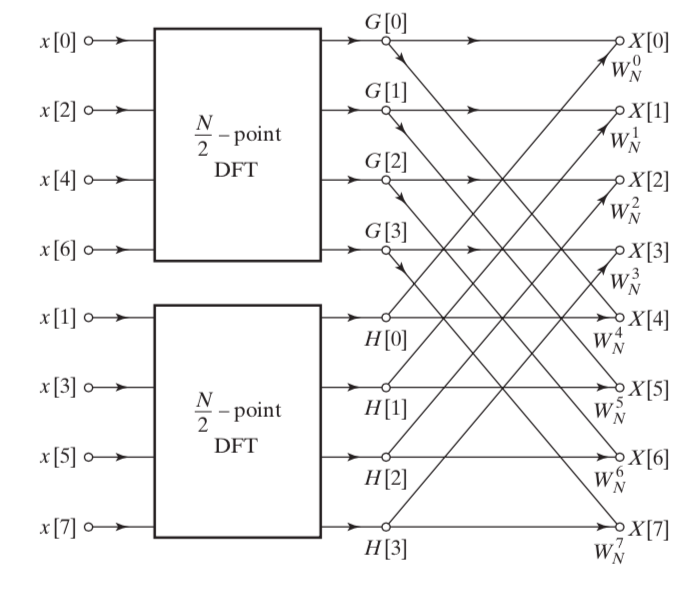
\includegraphics[scale=0.4]{fft_1.png}
    \caption{Representing an $N$-point DFT as two $\frac{N}{2}$-point DFT's with additional computation. [\textit{Image Source: Oppenheim and Schafer}.]}
    \label{fft_1}
\end{figure}

We can further break the $\frac{N}{2}$ point DFT's into two $\frac{N}{4}$-point DFT's. We also use the fact that $W_{\nicefrac{N}{2}}^{k} = W_{N}^{2k}$. This structre is shown in Figure \ref{fig:fft_2}.


\begin{figure}[!h]
    \centering
    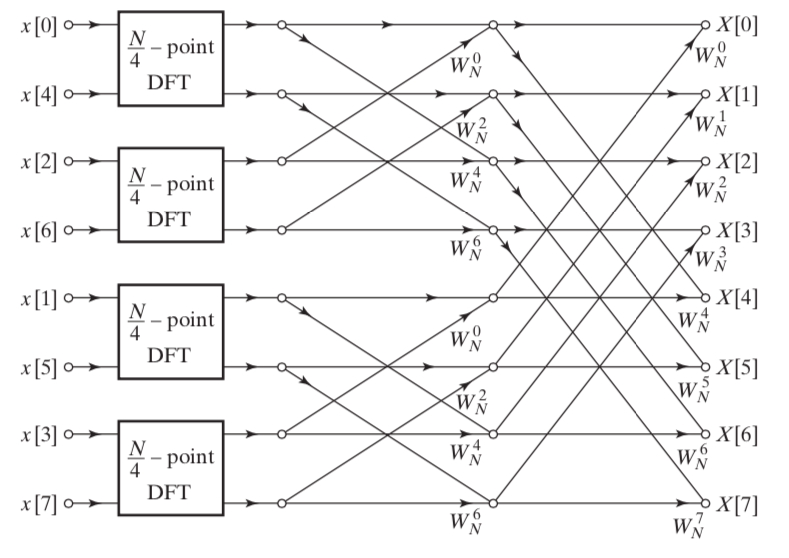
\includegraphics[scale=0.4]{fft_2.png}
    \caption{Representing an $N$-point DFT as four $\frac{N}{4}$-point DFT's with additional computation. [\textit{Image Source: Oppenheim and Schafer}.]}
    \label{fig:fft_2}
\end{figure}

We now use this decomposition recursively. The base case is a one-point DFT, which amounts to doing nothing. The complete signal flow graph is shown for $N=8$ in Figure \ref{fig:fft_time}. We use the following two identities
\[
    W_{N}^{\nicefrac{N}{2}} = -1 ; \quad W_{N}^{r+\nicefrac{N}{2}} = -W_{N}^{r}
\]
This leads to alternate additions and subtractions in $G[k]$ and $H[k]$. These alternate additions and subtractions constitute a butterfly-like structure in signal flow graphs. Hence, these are called butterfly computations. \medskip

\begin{figure}[!h]
    \centering
    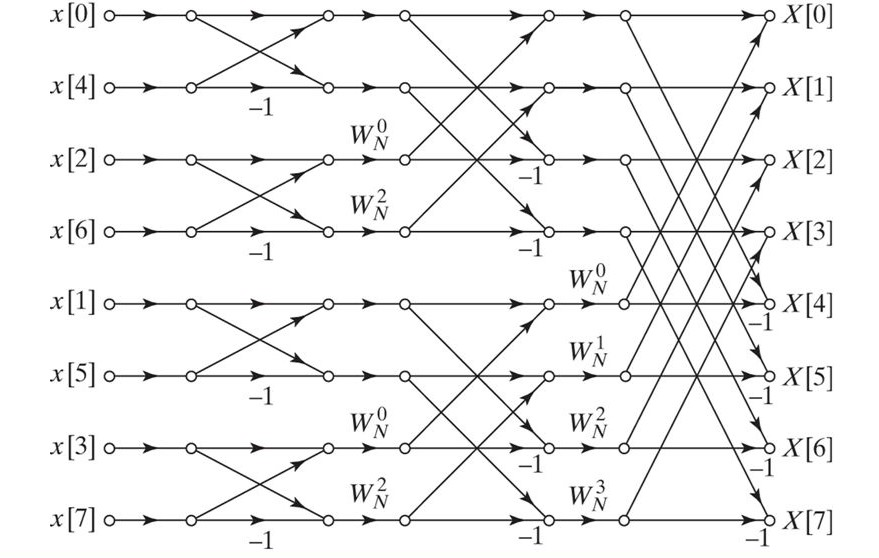
\includegraphics[scale = 0.4]{fft_time.jpg}
    \caption{Complete signal flow graph for the decimation-in-time structure. $W_{N}^{i}$ are the multipliers for different $k$. [\textit{Image Source: Oppenheim and Schafer}.]}
    \label{fig:fft_time}
\end{figure}

Note that to correctly implement this algorithm, we must ensure correct `arrangement' of $n$ at every stage. To find out the initial configuration, we represent $n$ in the binary format. Note that alternating even and odd samples in $n$ can be represented by a \textit{cyclic shift of bits} from the regular ordering of $n$. As this cyclic shift is carried out $3$ times for $N=8$, we represent the $n$'s in the thrice-shifted bit format. Note that this is the same as \textit{reversing} the bits. Hence, for any general $N$, $n$ is written in bit-reversed indexing. For $N=8$, the initial arrangement of $n$ is as follows 
\[
    n = {[} 0, 4, 2, 6, 1,5,3,7 {]}
\]

\subsection{Computational Complexity}

We have devised the FFT algorithm, but is it really efficient? We now compare its computational complexity with a direct computation of the DFT. Note: We consider multiplication by $1$ and $-1$ to be trivial multiplications and they do not contribute to computational complexity. \medskip

For $N=8$, the FFT algorithm involves $5$ non trivial multiplications and $24$ additions. We represent this as the tuple $(5,24)$. The direct computation of the DFT uses the formula 
\[
    X[k] = \sum_{n=0}^{7} x[n] \cdot e^{-j \frac{2\pi}{8} nk}
\]

The number of additions is $8 \times 7 = 56$. To find out the number of non trivial multiplications is a bit more tricky. Multiplication by $\exp -j \frac{2\pi}{N} nk$ will be trivial if and only if $nk$ is a multiple of $4$. To find the number of pairs $(n,k)$ which cause a trivial multiplication, we construct the following table, shown in Table \ref{table:nk}.

\begin{table}[H]
    \begin{adjustbox}{center}
    \begin{tabular}{|c|c|c|c|c|c|c|c|c|}
        \hline
        n \textbackslash \; k & 0 & 1 & 2 & 3 & 4 & 5 & 6 & 7 \\
        \hline
        0 & \cellcolor{shade} & \cellcolor{shade} & \cellcolor{shade} & \cellcolor{shade} & \cellcolor{shade} & \cellcolor{shade} & \cellcolor{shade} & \cellcolor{shade} \\
        \hline
        1 & \cellcolor{shade} & & & & \cellcolor{shade} & & & \\
        \hline
        2 & \cellcolor{shade} & &\cellcolor{shade} & & \cellcolor{shade} & & \cellcolor{shade}& \\
        \hline
        3 & \cellcolor{shade} & & & & \cellcolor{shade} & & & \\
        \hline
        4 & \cellcolor{shade} & \cellcolor{shade} & \cellcolor{shade} & \cellcolor{shade} & \cellcolor{shade} & \cellcolor{shade} & \cellcolor{shade} & \cellcolor{shade} \\
        \hline
        5 & \cellcolor{shade} & & & & \cellcolor{shade} & & & \\
        \hline
        6 & \cellcolor{shade} & &\cellcolor{shade} & & \cellcolor{shade} & & \cellcolor{shade}& \\
        \hline
        7 & \cellcolor{shade} & & & & \cellcolor{shade} & & & \\
        \hline
    \end{tabular}
    \end{adjustbox}
    \caption{Table for $(n,k)$. The shaded boxes denote trivial multiplications.}
    \label{table:nk}
\end{table}

Hence, the number of non-trivial multiplications is $32$. Thus, the tuple corresponding to the direct computation is $(32,56)$. This is much worse than the FFT tuple. \medskip

In general, for $N = 2^p$, we have $\frac{N}{2}$ non trivial multiplications and $N$ additions per stage, and we have $p$ stage. While, for the direct computation, we have $N(N-1)$ additions and $N^2$ multiplications. Hence, the complexity for the FFT algorithm is $\mathcal{O}(N \log N)$ while the complexity for the direct computation is $\mathcal{O}(N^2)$. Hence, the FFT is much more efficient. \medskip

The second approach involves partitioning $n$ and picking alternate $k$. This is known as a \textbf{Decimation-in-Frequency} structure. It is not to difficult to show that the signal flow graph for this method is the \textit{same} as the decimation-in-time structure but with all the arrows reversed. We say that the graph for the decimation-in-frequency structure is the \textit{transpose} of the graph for the decimation-in-time structure. We can also prove that the computational complexity remains unchanged. The complete signal flow graph for the decimation-in-frequency structure is shown for $N=8$ in Figure \ref{fig:fft_freq}. Note: We could perform a bit-reversed indexing here as well. 


\begin{figure}[!h]
    \centering
    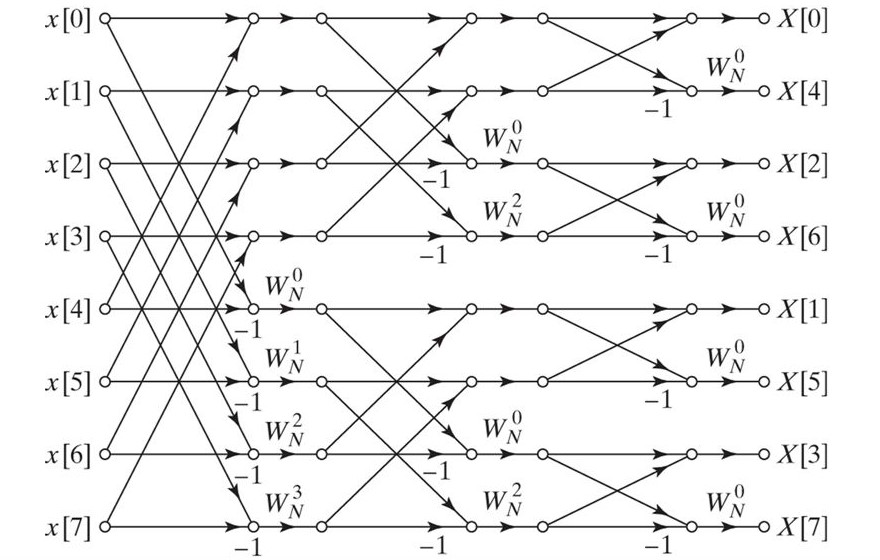
\includegraphics[scale=0.5]{fft_freq.jpg}
    \caption{Complete signal flow graph for the decimation-in-frequency structure. [\textit{Image Source: Oppenheim and Schafer}.]}
    \label{fig:fft_freq}
\end{figure}

An interesting thing to note is that the FFT algorithm can also be used to calculate the Inverse DFT. The expression remains the same for both cases, except for an additional factor of $\frac{1}{N}$. 

\subsection{Computing Convolutions using the FFT Algorithm}

Consider that we wish to compute the convolution of a $15$-point sequence $x_1[n]$ with a $14$-point sequence $x_2[n]$. The number of points in the convolved sequence $y[n]$ will be $28$. We can compute the convolution in two ways :
\begin{itemize}
    \item Direct Computation:
    \[
        y[n] = \sum_{k=-\infty}^{\infty} x_1[n] \cdot x_2[n-k]
    \]
    \item Computation through FFT:
    \[
        y[n] = \text{IFFT}_{N} \left( \text{FFT}_{N}(x_1[n]) \cdot \text{FFT}_{N} \right)
    \]
    where $\text{FFT}_{N}$ and $\text{IFFT}_{N}$ are the $N$-point FFT and Inverse FFT algorithms respectively. 
\end{itemize}

How do these two methods compare in terms of computation required? We now only focus our attention on the number of multiplications required. The direct computation involves $15 \times 14 = 210$ multiplications. While using FFT, we must choose $N$ such that $N \geq 28$. The nearest power of $2$ is $32$, hence we use a $32$-point FFT. The sequence $x_1[n]$ is padded with $17$ zeroes and the sequence $x_2[n]$ is padded with $18$ zeroes. The number of multiplications required are $32 \times \logtwo 32 = 32 \times 5$ for each of the two inputs and the output. Hence, the total number of multiplications required is $32 \times 15 = 480$. This seems to be larger than the direct computation. However, note that more than half of both our sequences are zeroes. Hence, many of the multiplications would turn out to be trivial. This would greatly reduce the number of multiplications required. Further, our output is $32$ points long but we only need to be concerned with the first $28$. This would also reduce the computation. Thus, the two methods are more or less comparable in their computations. \medskip

As such, the FFT Algorithm does not seem to be providing us any distinct advantage. However, we have chosen a very small value of $N$. Consider now that we have a $200$-point and a $300$-point sequence. The output is roughly $500$ points long ($499$ to be precise). The number of multiplications required in the direct computation is $300 \times 200 = 60,000$. We would have to work with a $512$-point FFT. The total number of multiplications would then be $512 \times \logtwo 512 \times 3 = 13,824$. However, note that the multiplications in the direct computation are \textit{real} multiplications while those in the FFT are \textit{complex} multiplications (for real sequences). A complex multiplication is roughly $4$ real multiplications. Hence, the number of multiplications in the FFT algorithm would be $13,824 \times 4 = 55,296$. This is still better than the direct computation. \medskip

The advantage provided by the FFT is still not significant. Let us consider a larger value of $N$. Consider that we have two $1,000$-point sequences. The output is roughly $2,000$ points long (precisely $1,999$). We hence use a $2,048$-point FFT. The number of multiplications in the direct computation are $1,000 \times 1,000 = 10,00,000$. For the FFT, we again consider $4$ multiplications per complex multiplication. The total number of multiplications are then $2,048 \times \logtwo 2,048 \times 3 \times 4 = 2,70,336$. This is significantly better than the direct computation. Hence, for larger and larger sequences, the FFT is more and more efficient.

\subsection{Generalised FFT Algorithm for composite $N$}

So far, we have only discussed the FFT Algorithm when $N$ was a power of $2$. Let us consider a composite value of $N$. Let $N= N_1 N_2$ where $N_1$ and $N_2$ are positive integers greater than $1$. We now use two indices $n_1,n_2$ in place of $n$ and $k_1,k_2$ in place of $k$. These are related as
\[
    n = N_2 n_1 + n_2 \quad
    \begin{cases}
        n_1 = 0, \ldots , N_1 - 1 & \\
        n_2 = 0, \ldots , N_2 - 1 
    \end{cases}
\]
\[
    k = k_1 + N_1 k_2 \quad
    \begin{cases}
        k_1 = 0, \ldots , N_1 - 1 & \\
        k_2 = 0, \ldots , N_2 - 1 
    \end{cases}
\]

After simplifying the DFT, we get 
\[
    X[k_1 + N_1 k_2] = \sum_{n_2=0}^{N_2 -1} \left[ \left( \sum_{n_1=0}^{N_1 -1} x[N_2n_1 + n_2] W_{N_1}^{k_1n_1} \right) W_{N}^{k_1n_2} \right] W_{N_2}^{k_2n_2}
\]

We interpret this as follows: First, we take $N_2$ $N_1$-point DFTs. These are then modified by the twiddle factors $W_{N}^{k_1n_2}$. Then, we take $N_1$ $N_2$-point DFTs. This method can then be used recursively to compute the $N_1$ and $N_2$ point DFTs as well. This method also has a complexity of $\mathcal{O}(N \log N)$.



%



\begin{thebibliography}{9}
\bibitem{vmglecs}
Lectures by Prof. Vikram M Gadre on the course \textit{EE603 - Digital Signal Processing and its Applications}. 
Autumn, 2009.
\bibitem{opschaf}
Alan V. Oppenheim and Ronald W. Schafer, \textit{Discrete-Time Signal Processing}.
Pearson, 2009.
\bibitem{dspguide}
Steven W. Smith, \textit{The Scientist and Engineer's Guide to Digital Signal Processing}. 
\\\texttt{http://www.dspguide.com/}
\end{thebibliography}
\end{document} 
